Two data-driven methods are used to estimate the FNP lepton background, referred to as the ``matrix method'' and the ``MC template method''.
The estimates from these methods are combined to give the final estimate. 
To follow the discussion of Chapter~\ref{chap:fake}, 
this section gives more detail on the application of the two methods in this analysis.

\subsection{Matrix Method}
The matrix method relates the number of events containing prompt or FNP leptons 
to the number of observed events with tight or loose-not-tight leptons 
using the probability for loose prompt or FNP leptons to satisfy the tight criteria.
The formalism for this method has been discussed in Section~\ref{sec:fake.mxm}.
The next sections will concentrate on the measurement of the 
two input variables needed for the matrix method:
the probability for loose FNP leptons to satisfy the tight selection
criteria ($\zeta$) and 
the probability for loose prompt leptons to satisfy the tight selection 
criteria ($\varepsilon$).

\subsection*{Baseline-to-signal efficiency for fake muons}

Baseline-to-signal efficiency for fake leptons (further called ``fake rate'', ($\zeta$)) is measured 
in a sample enriched in fake leptons from \ttbar\ processes.
The MC simulations indicate that this background has the largest contribution to FNP lepton background in the signal regions, 
even those with $b$-jet vetoes, due to the requirements on jet multiplicity and \met. 
The events used for the measurements require exactly two same-sign muons (and no extra baseline lepton), 
at least one $b$-jet, and at least 3 jets that were acquired by di-muon triggers.
One of the muons in the event (referred to as ``tag'') is required to satisfy signal requirements, verify $\pt>25~\GeV$, 
and trigger the event recording. 
The measurement may then be performed on the other lepton (``probe''), likely to be the fake lepton of the pair. 

%%
\begin{figure}[t!]
\centering
\begin{tabular}{rr}
\begin{subfigure}[t]{0.5\textwidth}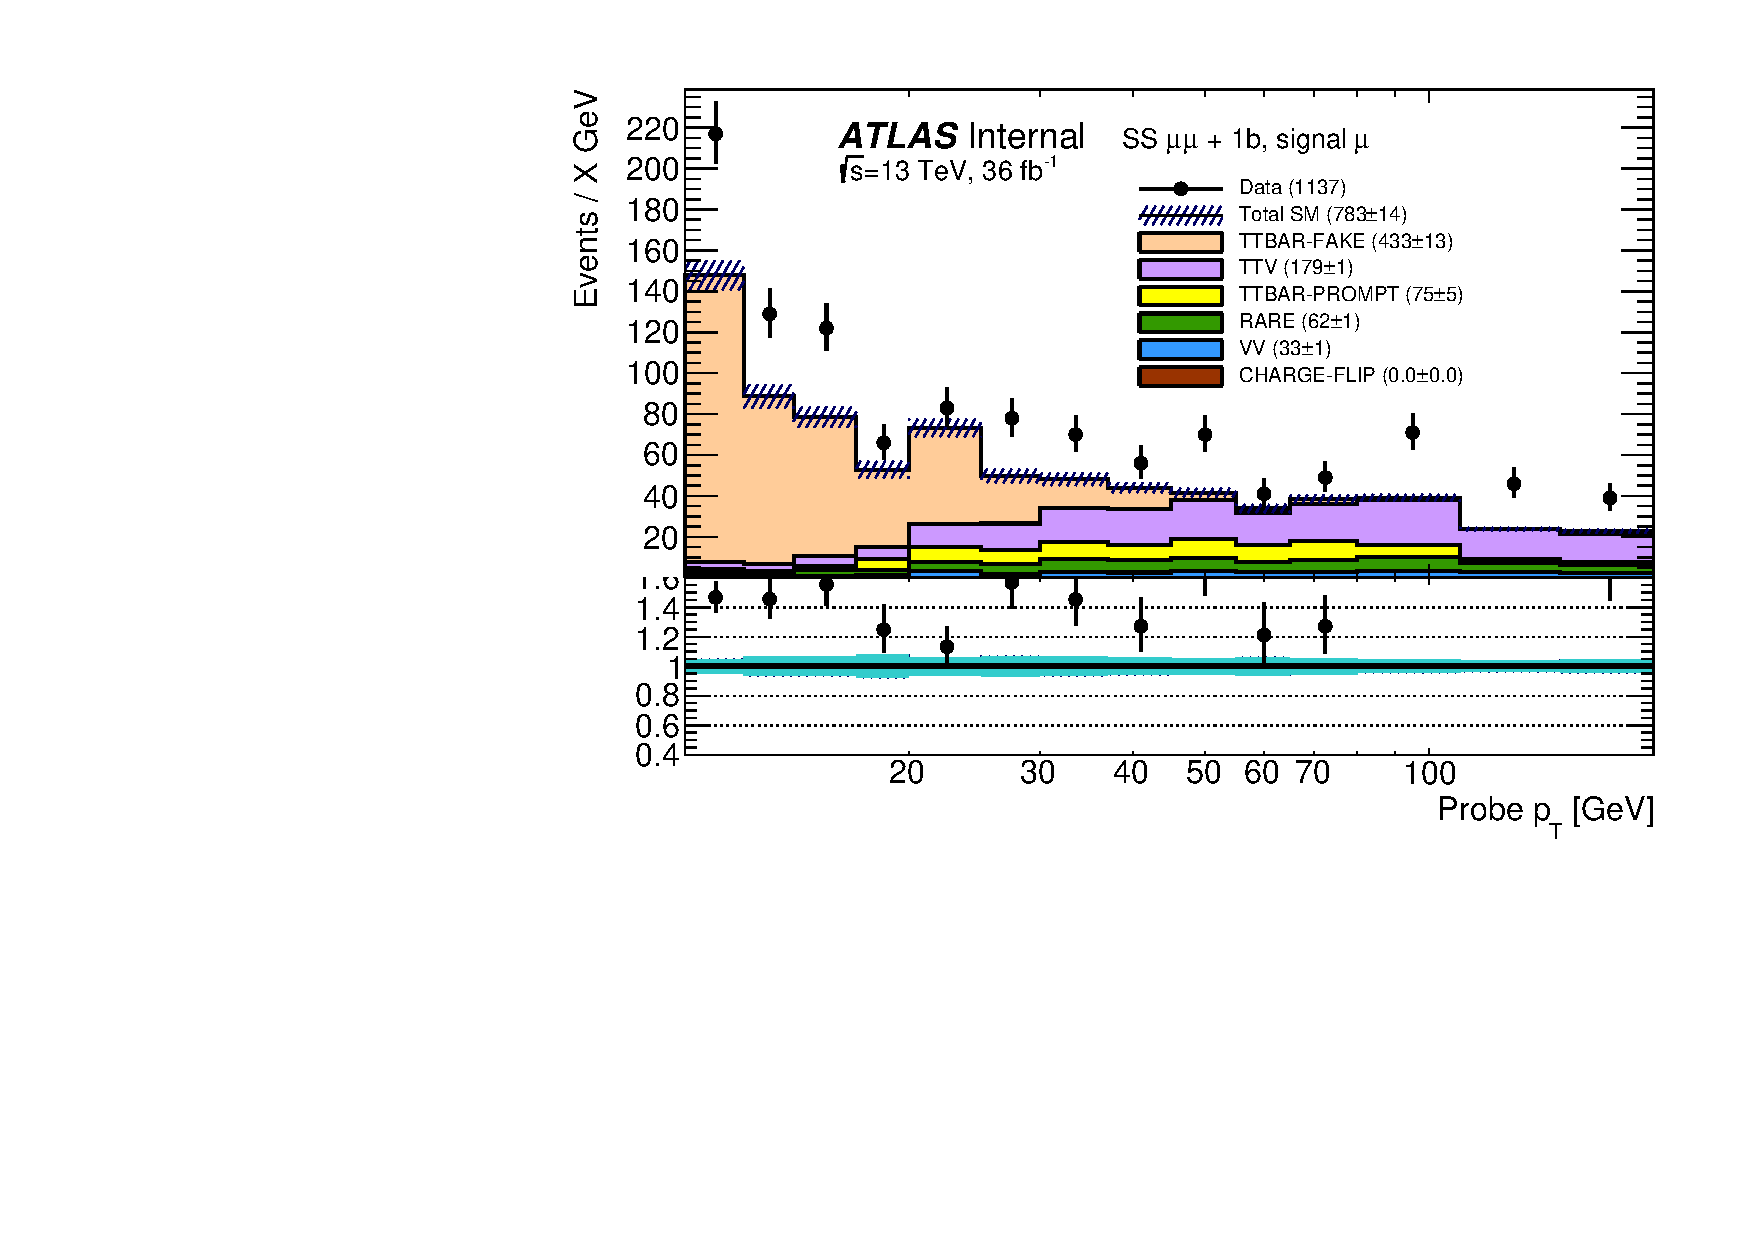
\includegraphics[width=\textwidth]{INCLUSIVETAG_PROBE_PT_MUON_SIGNAL}\caption{}\label{fig:bkg.mxm.INCLUSIVETAG_PROBE_PT_MUON_SIGNAL}\end{subfigure}&
\begin{subfigure}[t]{0.5\textwidth}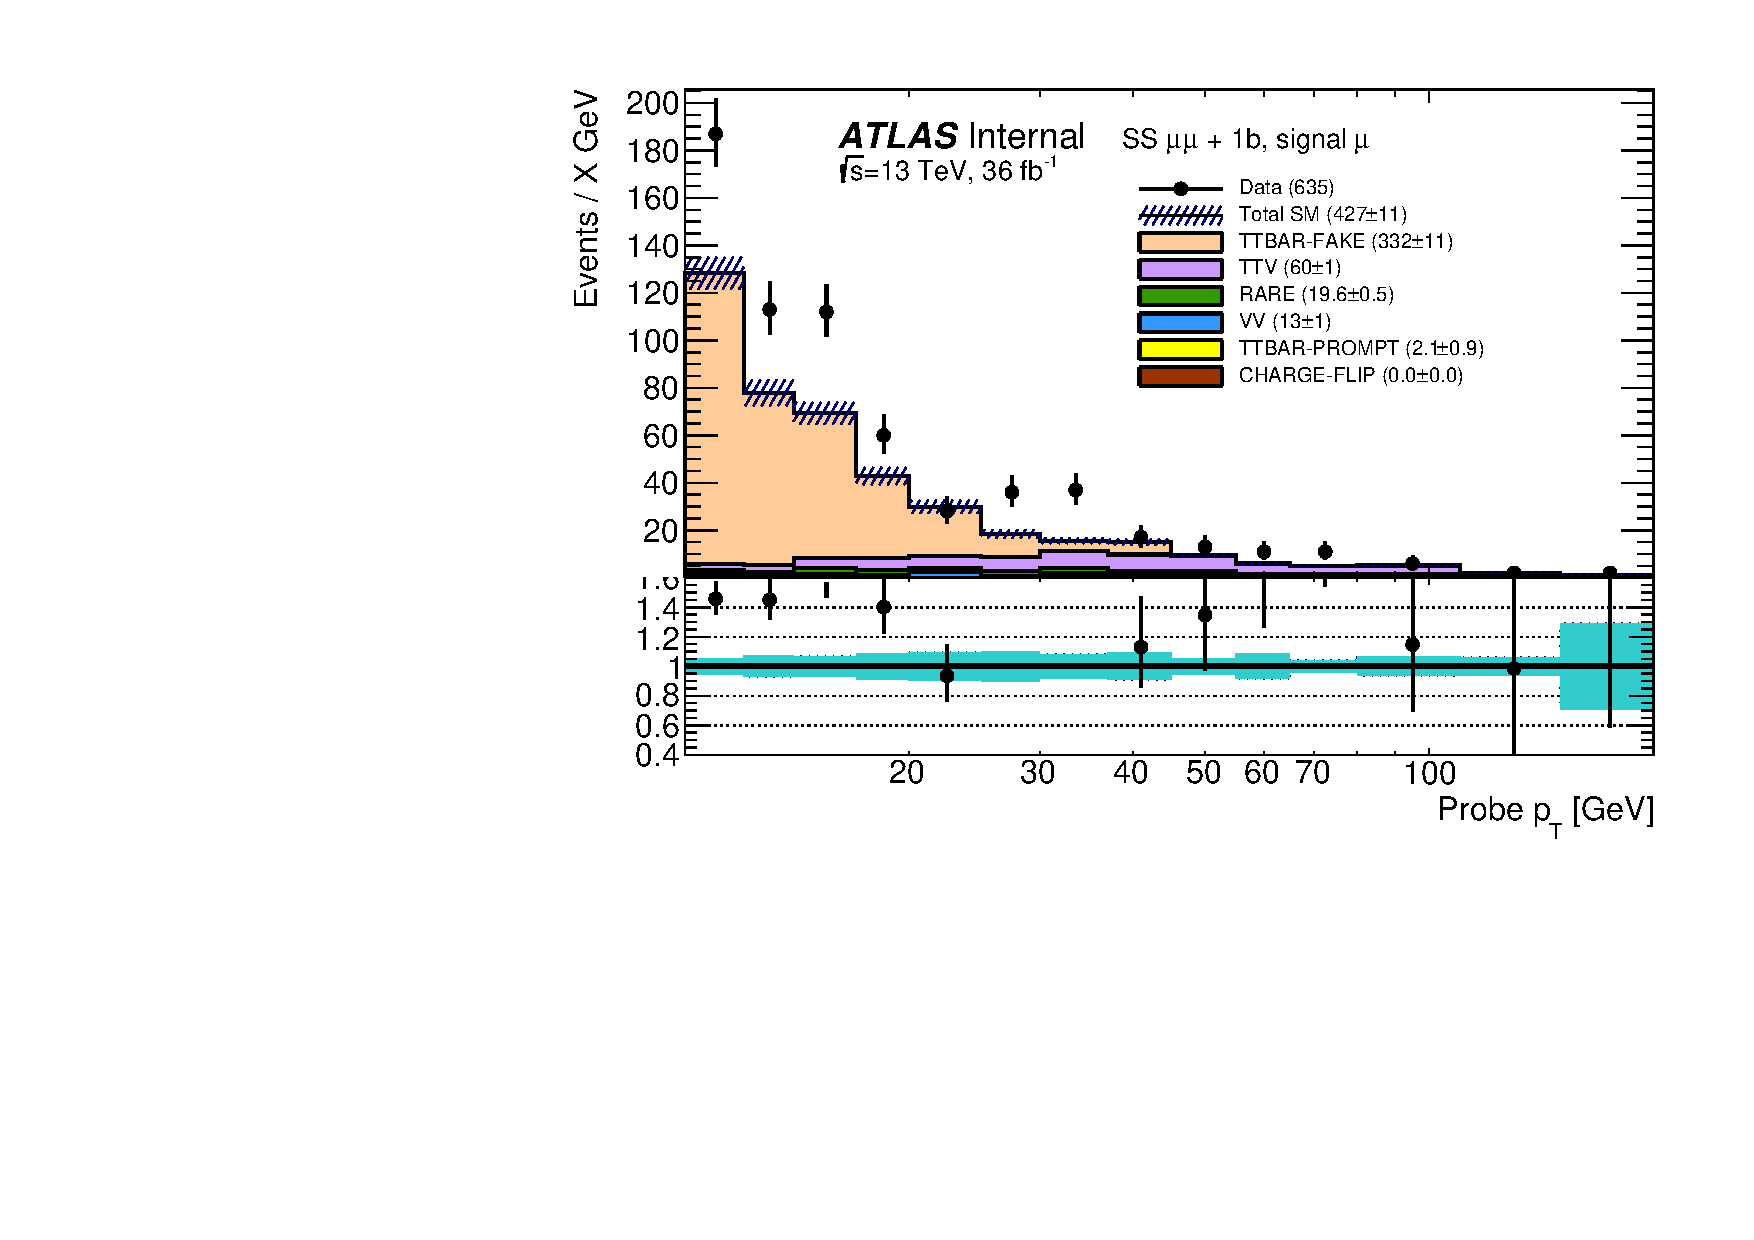
\includegraphics[width=\textwidth]{IDEALTAG_PROBE_PT_MUON_SIGNAL}\caption{}\label{fig:bkg.mxm.IDEALTAG_PROBE_PT_MUON_SIGNAL}\end{subfigure} \\
\end{tabular}
\caption
{Signal probe muon \pt\ distribution in data and MC, after pre-selection (left) 
or further tightening of the tag muon requirements (right).
The yellow area indicates $t\bar t$ events in which the tag muon is fake and the probe real, 
leading to a measurement bias. 
}
\label{Fig:fakes_preselection_muon}
\end{figure}
%%

Figure~\ref{fig:bkg.mxm.INCLUSIVETAG_PROBE_PT_MUON_SIGNAL} shows the number of signal muon probes available after this pre-selection. 
It is clear that at this stage, measurements above 25 \GeV~would be very affected by the important fraction of events 
in which the tag muon is fake and the probe muon is real. 
To overcome this issue, two alternatives are considered: 
\begin{itemize}
\item tighten the \pt\ and isolation requirements of the tag muon beyond the ``signal'' requirements,
to reduce its probability of being a fake muon
\item use an identical selection for tag and probe muons, and require them to be in the same (\pt,$\eta$) bin for the measurement; 
after subtraction of estimated contributions from processes with two prompt muons, all events have one real and one fake muon, 
and the symmetry in the muon selection can be taken advantage of to obtain an unbiased measurement of the fake rate: 
$$
\zeta = \frac{\varepsilon n_2}{\varepsilon n_1+(2\varepsilon-1)n_2}
$$
%\text{ with }n_1, n_2\text{ the number of events with 1 or 2 signal muons}, 
%\text{ and }\varepsilon\text{ the efficiency for prompt muons.}
with $n_1, n_2$ the number of events with 1 or 2 signal muons, 
and $\varepsilon$ the efficiency for prompt muons.

This method is limited to measurements in inclusive or wide bins. 
It also can't be used at too low \pt, due to contributions from processes with two fake muons (e.g. from $B\bar B$ meson production). 
\end{itemize}
Comparisons made with $t\bar t$ MC indicated that when using a very tight isolation requirement on the tag muon 
($\operatorname{max}(E_\mathrm{T}^\text{topo, cone 40},p_\mathrm{T}^\text{cone 40})<0.02\times\pt$), 
the level of bias is always largely inferior to the statistical uncertainty in the measurement, 
which itself is smaller than for the other two methods. 

Figure~\ref{fig:bkg.mxm.IDEALTAG_PROBE_PT_MUON_SIGNAL} shows the number of signal muon probes when applying those reinforced isolation criteria to the tag muon, 
as well as requiring $p_\mathrm{T}^\text{tag}>\operatorname{max}(40,p_\mathrm{T}^\text{probe}+10)$~\GeV. 
As expected, the number of pairs with a fake tag muons is down to a minor level, at least according to the simulation. 

%%
\begin{figure}[t!]
\centering
\begin{tabular}{rr}
\begin{subfigure}[t]{0.5\textwidth}\includegraphics[width=\textwidth]{{TTBAR.Incl.FakeRate.Muon}.pdf}\caption{}\label{fig:TTBAR.Incl.FakeRate.Muon}\end{subfigure}&
\begin{subfigure}[t]{0.5\textwidth}\includegraphics[width=\textwidth]{{TTBAR.Incl.FakeRateVsEta.Muon}.pdf}\caption{}\label{fig:TTBAR.Incl.FakeRateVsEta.Muon}\end{subfigure} \\
\end{tabular}
\caption
{
Muon fake rates in $t\bar t$ MC with an inclusive selection, 
as function of \pt\ (left, green markers) or $|\eta|$ in different momentum ranges (right). 
}
\label{Fig:fakes_MC_inclusive_rates_muon}
\end{figure}
%%

Muon fake rates as predicted by the simulation ($t\bar t$, inclusive selection of leptons via truth-matching) 
are shown on Fig.~\ref{Fig:fakes_MC_inclusive_rates_muon} as function of \pt\ and $|\eta|$. 
One can expect a moderate dependency of the fake rates to the transverse momentum, with the strongest evolution at low \pt and a slight increase toward higher \pt. 
The fake rates are also essentially independent of the pseudorapidity, 
except at the edge ($|\eta|>2.3$) where there is a strongly pronounced increase of the rates. 
This motivates measurements in data as function of \pt\ in two $|\eta|$ bins. 

Observations in data seem to indicate that the rejection of fake tag muons by the reinforced isolation criteria 
is quite less important than in the simulation, or that the amount of fake muons at high \pt\ is larger than in the simulation, or both. 
This leads to an unknown level of bias in measurements performed with the straightforward tag-and-probe selection at high \pt. 
For that reason, the final rates measured in data are provided by the tag-and-probe method below 25~\GeV, 
and by the symmetric selection for $\pt>25~\GeV$. The former are obtained with 

\begin{align}
\zeta&=\frac{n_\text{signal}^\text{data} - n_\text{signal}^\text{MC}}{n_\text{baseline}^\text{data} - n_\text{baseline}^\text{MC}}\\
\text{with }&\Delta\zeta_\text{stat} = \frac{\sqrt{(1-2\zeta)n_\text{signal}^\text{data} + \zeta^2 n_\text{baseline}^\text{data}}}
{n_\text{baseline}^\text{data} - n_\text{baseline}^\text{MC}}\notag
%\text{and }&\Delta\zeta_\text{syst} = \frac{\Delta B}{B}\times\frac{\sqrt{(1-\zeta^2)(n_\text{signal}^\text{MC})^2 
%+ \zeta^2 (n_\text{baseline}^\text{MC} - n_\text{signal}^\text{MC})^2 }}
\end{align}
while the latter are obtained with:
\begin{align}
\zeta &= \frac{\varepsilon (n_\text{both signal}^\text{data} - n_\text{both signal}^\text{MC})}
{\varepsilon (n_\text{only 1 signal}^\text{data} - n_\text{only 1 signal}^\text{MC})
+(2\varepsilon-1)(n_\text{both signal}^\text{data} - n_\text{both signal}^\text{MC})}\\
\text{with }&\Delta\zeta_\text{stat} 
= \frac{\zeta}{n_\text{both signal}^\text{data} - n_\text{both signal}^\text{MC}}
\sqrt{\zeta^2 n_\text{only 1 signal} + \left(1-\frac{2\varepsilon-1}{\varepsilon}\zeta\right)^2 n_\text{both signal}}\notag
\end{align}
the efficiency for prompt muons $\varepsilon$ is assigned values compatible with section~\ref{subsubsec:fakes_matrix_real_efficiency}. 

The measured rates are presented in Table~\ref{table:fake_rates_muon}. 
The central values are shown together with the associated statistical uncertainty, 
as well as the propagation of the uncertainty on the subtracted backgrounds normalization, 
which is taken as a global $\Delta B/B=20\%$. 
The rates are of the order of $10\%$ up to 30 \GeV, beyond which they increase. 
Overall these values are not very different from those predicted by the simulation. 

%%
\begin{table}[t!]
\def\arraystretch{1.15}
\caption{Muon fake rate measured in data and the associated statistical uncertainty. 
The systematic uncertainty originating from the subtraction of ``backgrounds'' with only prompt leptons is also displayed. }
\label{table:fake_rates_muon}
\def\arraystretch{1.15}
\centering
\resizebox{\textwidth}{!}{
\begin{tabular}{|c|c|c|c|} \hline\hline
\multicolumn{2}{|c|}{$10<\pt<12~\GeV$}         & \multicolumn{2}{c|}{$12<\pt<14$}                  \\   
$|\eta|<2.3$             & $|\eta|>2.3$             & $|\eta|<2.3$             & $|\eta|>2.3$            \\
$0.14 \pm 0.01 \pm 0.00$ & $0.22 \pm 0.05 \pm 0.00$ & $0.11 \pm 0.01 \pm 0.00$ & $0.24 \pm 0.06 \pm 0.00$ \\ 
\hline \hline
\end{tabular}}

\resizebox{\textwidth}{!}{
\begin{tabular}{|c|c|c|c|} \hline\hline
\multicolumn{2}{|c|}{$14<\pt<17$}                    & \multicolumn{2}{c|}{$17<\pt< 20~\GeV$}       \\       
$|\eta|<2.3$             & $|\eta|>2.3$             & $|\eta|<2.3$             & $|\eta|>2.3$            \\    
$0.12 \pm 0.01 \pm 0.00$ & $0.09 \pm 0.05 \pm 0.00$ & $0.09 \pm 0.01 \pm 0.00$ & $0.21 \pm 0.07 \pm 0.00$ \\
\hline \hline
\end{tabular}}

\resizebox{\textwidth}{!}{
\begin{tabular}{|c|c|c|c|c|} \hline\hline
             $20<\pt<30$ &              $30<\pt<40$ &              $40<\pt<60$ &                $\pt>60$ \\
$0.07 \pm 0.02 \pm 0.00$ & $0.12 \pm 0.05 \pm 0.01$ & $0.16 \pm 0.09 \pm 0.04$ & $0.49 \pm 0.10 \pm 0.07$ \\
\hline \hline
\end{tabular}}

\end{table}

Some of the validation and signal regions require events with 2 or more $b$-tagged jets, 
which reduces the fraction of non-prompt muons coming from $B$ meson decays. 
Figure~\ref{fig:fakes_MC_vsBjets_muon} illustrates how this impacts on the fake rates. 
Given the good agreement between data and simulation for the measured values, 
A correction is applied to the measured rates for events with $\ge 2$ $b$-jets, 
taken directly from simulated $t\bar t$ events. 
This correction factor varies between 1 and 2 with \pt, 
and the whole size of the correction is assigned as an additional systematic uncertainty (see Table~\ref{tab:fake_rates_muon_systematics}). 

\begin{table}[t!]
\def\arraystretch{1.15}
\caption{Additional systematic uncertainty on the muon fake rates, to address variations of the latter in different environments. 
The table also shows the correction factors and uncertainties applied to final states with $\ge 2$ $b$-tagged jets.}
\label{tab:fake_rates_muon_systematics}
\def\arraystretch{1.15}
\centering
\resizebox{\textwidth}{!}{
\begin{tabular}{|c|c|c|c|c|c|c|} \hline\hline
 \pt & $<14$ & $14-20$ & $20-30$ & $30-40$ & $40-60$ & $>60$\\\hline
$\Delta\zeta^\text{(syst)}$ & 30\% & 30\%  & 30\%     &  50\%   & \multicolumn{2}{c|}{
		\begin{tabular}{@{}c@{}}50\% for $H_\mathrm{T}<600$ \\ 70\% for $600<H_\mathrm{T}<1200$ \\85\% for $H_\mathrm{T}>1200$\end{tabular}} \\\hline
$\frac{\zeta_{\ge 2b}}{\zeta}$ & $1.2\pm 0.2$ & $1.5\pm 0.5$ & $1.7\pm 0.7$ & $2.0\pm 1.0$ & $1.5\pm 0.5$ & $-$\\\hline
\end{tabular}}
\end{table}


%%
\par{\bf Systematic uncertainties\\}
To cover potential differences in the fake rates between the measurement regions and the signal regions, 
that could be due to different origins or kinematic properties of the fake leptons, 
uncertainties are set based on the extent of those differences predicted by the simulation. 
The largest effect is the decrease of the fake rates with $H_\mathrm{T}$ (especially for high-\pt\ muons), 
which likely correlates to a harder jet at the origin of the non-prompt muon, hence a reduced likelihood to satisfy isolation requirements. 
Table~\ref{tab:fake_rates_muon_systematics} summarizes the additional systematic uncertainties applied to the muon fake rates. 
They vary from $30\%$ at low \pt, to up to 85\% for $\pt>40~\GeV$; in that range, the uncertainties are made $H_\mathrm{T}$-dependent. 

As already shown, Fig.~\ref{fig:fakes_MC_vsBjets_muon} shows the variation of the fake rate in $t\bar t$ MC as function of the number of $b$-tagged jets in the event. 
Unsurprisingly, the rates are very similar for $0b$ and $\ge 1b$ final states, 
justifying the use of the fake rates measured in this section (i.e. in a $\ge 1b$ region) to predict fake muon background in all signal regions. 

\begin{figure}[t!]
\centering
\includegraphics[width=0.49\textwidth]{{TTBAR.BjetImpact.FakeRate.Muon}.pdf}
\caption
{
Muon fake rates in $t\bar t$ MC with an inclusive selection, 
as function of \pt\ and split according to the number of $b$-tagged jets in the event. 
}
\label{fig:fakes_MC_vsBjets_muon}
\end{figure}

\subsection*{Baseline-to-signal efficiency for fake electrons}
\label{subsubsec:fakes_matrix_fake_rate_electrons}


%%
\begin{figure}[t!]
\centering
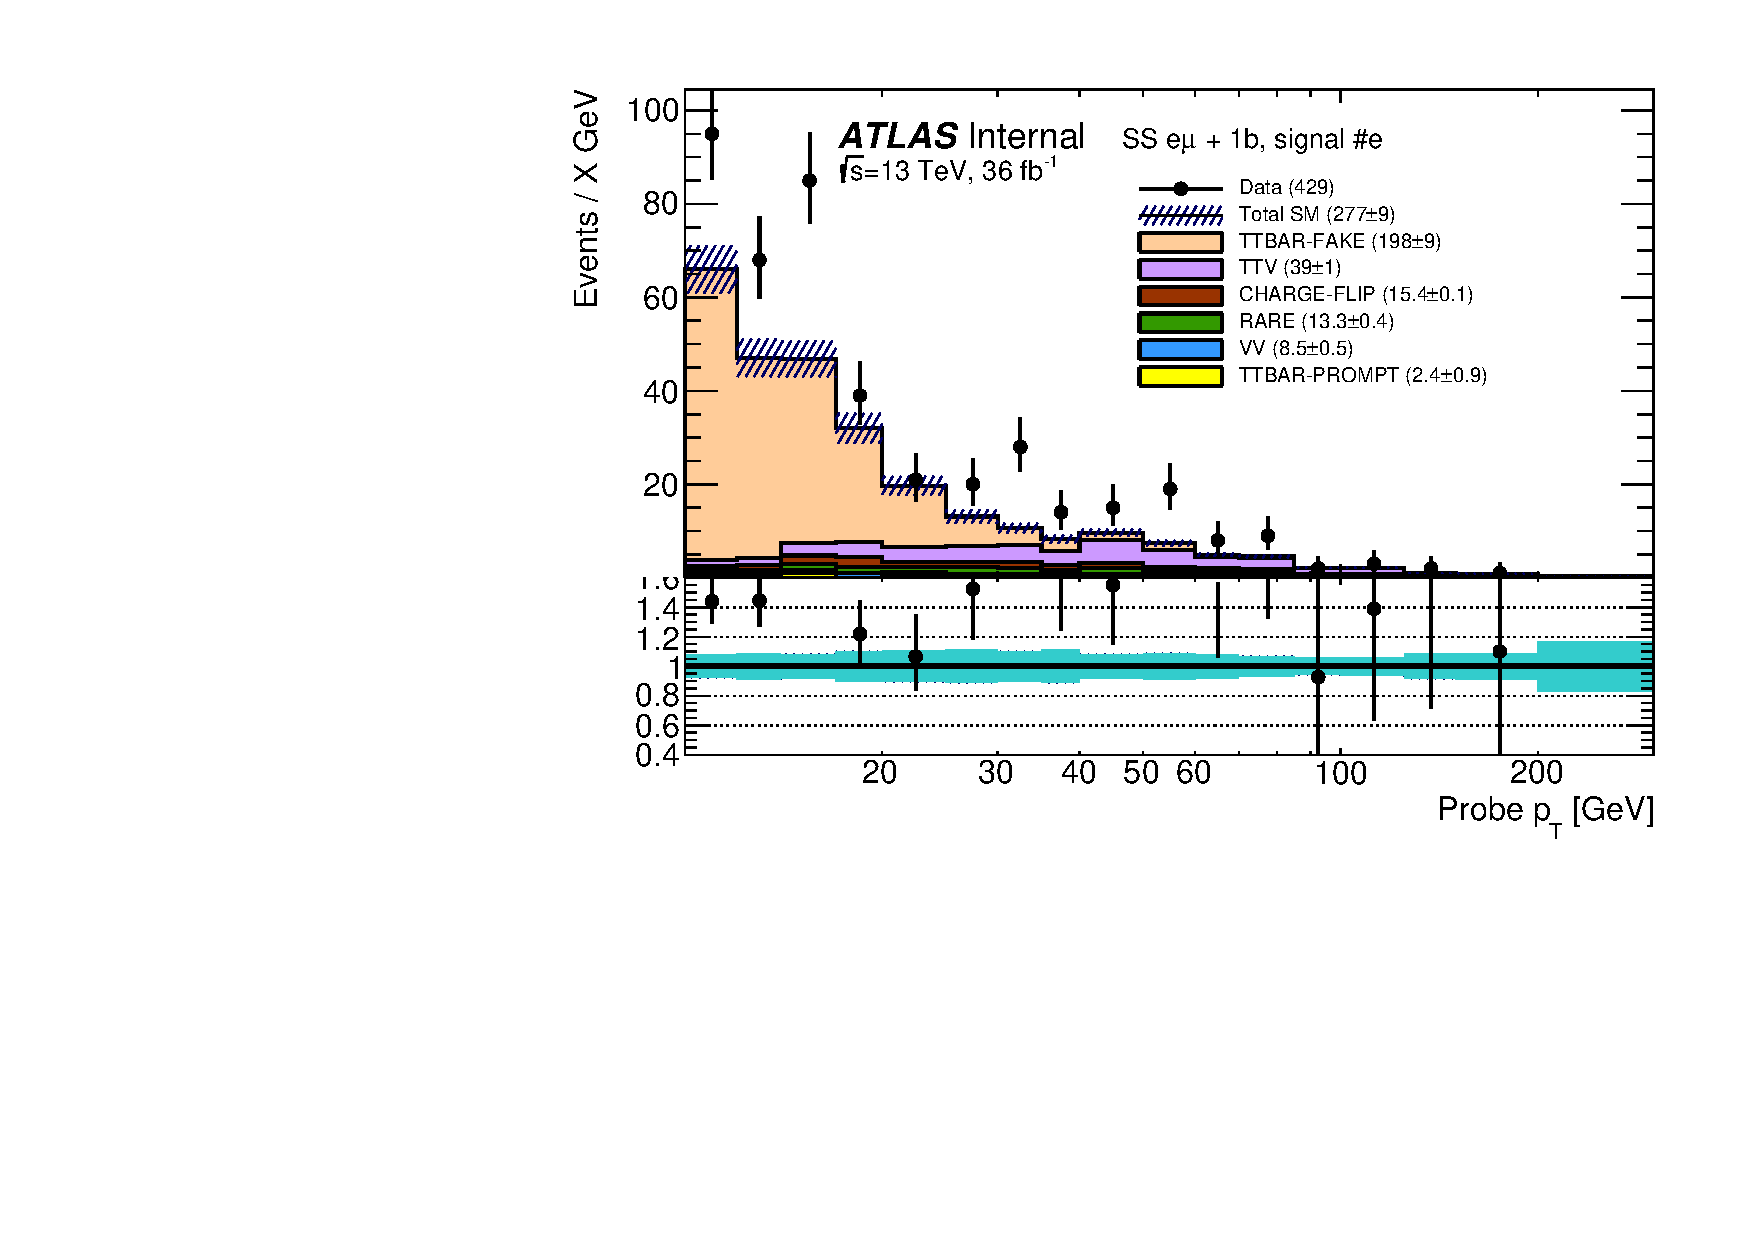
\includegraphics[width=0.49\textwidth]{IDEALTAG_CFTPROBE_PT_ELECTRON_SIGNAL}
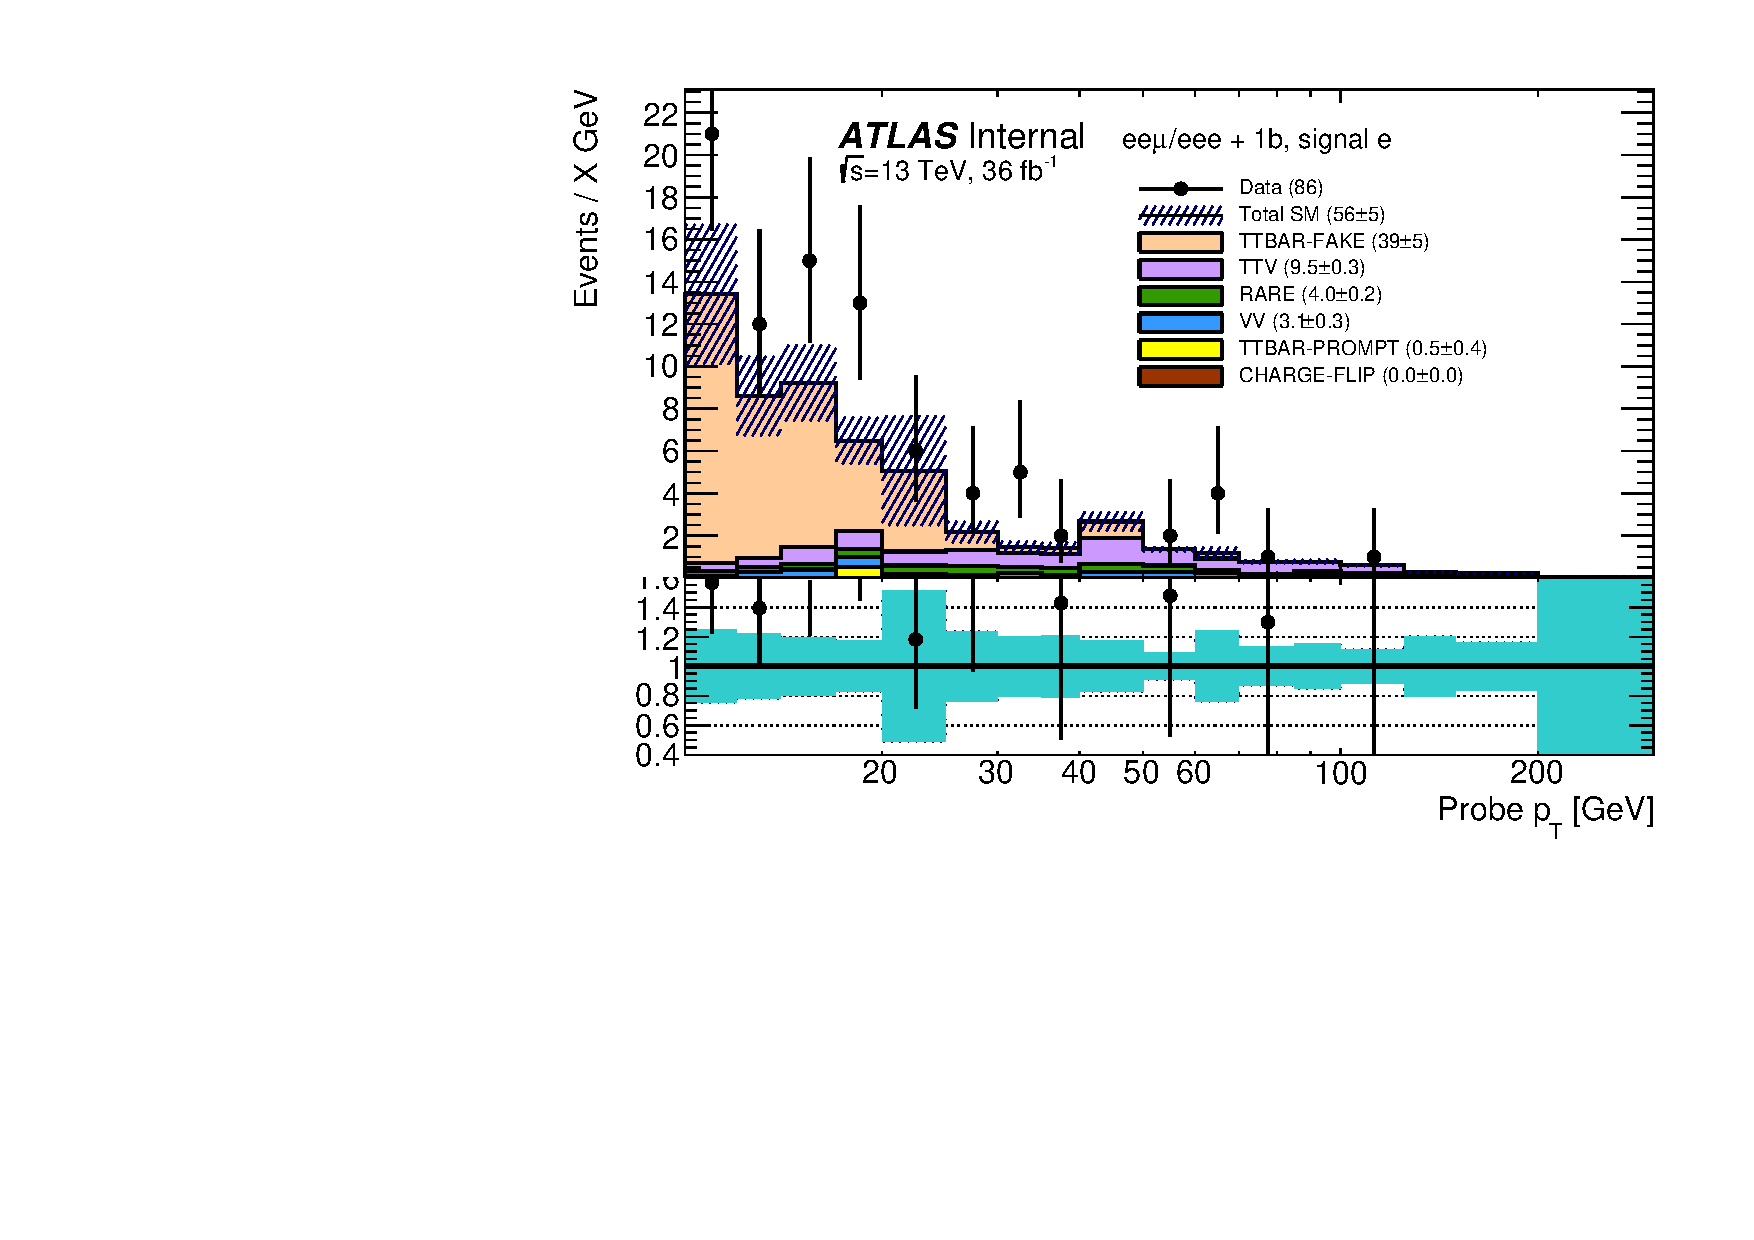
\includegraphics[width=0.49\textwidth]{TRILEP_IDEALTAG_PROBE_PT_ELECTRON_SIGNAL}
\caption
{Signal probe electron \pt\ distribution in data and MC, for $e^\pm\mu^\pm$ pairs (left, with probe electrons satisfying CFT cut and a reinforced tag muon selection) 
or $\ell^\pm e^\mp e^\mp$ pairs (right, with reinforced tag electron selection), 
as described in section~\ref{subsubsec:fakes_matrix_fake_rate_electrons}. 
The yellow area indicates $t\bar t$ events in which the tag lepton is fake and the probe electron real, 
leading to a measurement bias. 
}
\label{Fig:fakes_preselection_electron}
\end{figure}
%%

Electron fake rates are measured with a similar methodology, but the $e^\pm e^\pm$ channel is unusable due to the presence of a large charge-flip background. 
This is overcome by working with $e^\pm\mu^\pm$ pairs instead (with a tag muon), but mixing leptons of different flavours brings additional complications 
(for example, the unbiased measurement cannot be employed to measure muon fake rates at higher \pt, as there is no symmetry between the leptons). 
To improve confidence, measurements are performed in four different ways, which complement each other: 
\begin{itemize}
\item straightforward tag-and-probe with $e\mu$ pairs, with the same tag muon selection as in the previous section. 
\item same selection, but subtracting from the numerator the number of pairs with one fake tag muon and one prompt probe electron, 
itself estimated from the number of observed $e\mu$ events with a muon failing signal requirements, 
scaled by an efficiency correction factor $e\mu/\mu\mu$ taken from $t\bar t$ MC (only for pairs with one fake muon). 
This only works if the two muons satisfy the same kinematic requirements, therefore can be used only for measurements in wide or inclusive bins. 
\item selecting $\ell^\mp e^\pm e^\pm+\ge 1b$ events, with a $Z$ veto on SFOS pairs. 
This selection entirely suppresses contributions from charge-flip, or events with fake muons. 
One of the electron, with standard signal requirements, is required to satisfy the same reinforced \pt\ and isolation requirements as for the muon measurement,
and the measurement can be performed on the other electron. 
\item same selection, using the symmetry between the two same-sign electrons to measure the rates in an unbiased way, similarly to the muon case. 
\end{itemize}
Events are acquired with the combination of single-muon (as in previous section) and $e\mu$ triggers. 


Figure~\ref{Fig:fakes_preselection_electron} shows the number of signal probe electrons selected in the $e\mu$ and $\ell ee$ channels. 
There are quite less events selected in the trilepton channel. 
Figure~\ref{Fig:fakes_MC_inclusive_rates_electron} shows the electron fake rate as a function of \pt\ or $\eta$ in $t\bar t$ MC. 
The variations of the rates as function of the pseudorapidity are not very large, 
therefore measurements are only performed as a function of \pt. 
The low \pt\ range is dominated by non-prompt electrons from heavy flavour decays, while beyond 30~\GeV, 
electron fakes mostly come from conversions of photons produced inside jets, such as $\pi^0\to\gamma\gamma$ decays. 

%%
\begin{figure}[t!]
\centering
\includegraphics[width=0.49\textwidth]{{TTBAR.Incl.FakeRate.Electron}.pdf}
\includegraphics[width=0.49\textwidth]{{TTBAR.Incl.FakeRateVsEta.Electron}.pdf}
\caption
{
Electron fake rates in $t\bar t$ MC with an inclusive selection, 
as function of \pt\ (left, yellow/green markers = with/without CFT cut applied) or $|\eta|$ in different momentum ranges (right). 
}
\label{Fig:fakes_MC_inclusive_rates_electron}
\end{figure}
%%

Based on the estimated levels of bias, and achievable statistical precision, of the different methods, 
the electron fake rate is measured with the tag-and-probe $e\mu$ selection up to 30~\GeV, 
and by combining ``unbiased'' evaluations in both $e\mu$ and $\ell ee$ channels beyond. 
The measured rates are presented in Table~\ref{table:fake_rates_electron}, 
together with the associated statistical and background-subtraction uncertainties. 
The rates are of the order of $10\%$ up to 30 \GeV, beyond which they increase to up to 25\%. 

%%
\begin{table}[t!]
\def\arraystretch{1.15}
\caption{Electron fake rate measured in data and the associated statistical uncertainty. 
The systematic uncertainty originating from the subtraction of ``backgrounds'' with only prompt leptons is also displayed. }
\label{table:fake_rates_electron}
\def\arraystretch{1.15}
\centering
\resizebox{\textwidth}{!}{
\begin{tabular}{|c|c|c|c|} \hline\hline
             $10<\pt<12$ &              $12<\pt<14$ &              $14<\pt<17$ &             $17<\pt<20$ \\
$0.10 \pm 0.01 \pm 0.00$ & $0.10 \pm 0.01 \pm 0.01$ & $0.12 \pm 0.01 \pm 0.01$ & $0.08 \pm 0.02 \pm 0.00$ \\
\hline \hline
\end{tabular}}

\resizebox{\textwidth}{!}{
\begin{tabular}{|c|c|c|c|} \hline\hline
             $20<\pt<25$ &              $25<\pt<30$ &              $30<\pt<40$ &             $40>\pt$ \\
$0.07 \pm 0.02 \pm 0.01$ & $0.11 \pm 0.03 \pm 0.01$ & $0.20 \pm 0.07 \pm 0.03$ & $0.25 \pm 0.10 \pm 0.05$ \\
\hline \hline
\end{tabular}}

\end{table}

Unlike muons, MC-based correction factors are not applied for final states with $\ge 2$ $b$-tagged jets. 
This is because there is less good agreement between the measured rates and the simulation; 
in particular the former take larger values in the medium-\pt\ range. 

%%
\par{\bf Systematic uncertainties\\}

Similarly to the muon case, systematic uncertainties are assigned to cover for difference in the rates in the measurement regions and in the signal regions
that would be due to different sources of fake leptons, or different kinematic properties of these sources. 
Unlike muons, there is much less of a dependency to $H_\mathrm{T}$. 
The dominant source of potential differences is therefore the origin of the fake electron (see Fig.~\ref{fig:fakes_MC_perSource_electron}); 
for $\pt<20~\GeV$, non-prompt electrons from heavy--flavor hadron decays dominate,
which is confirmed by the good agreement between MC fake rates and those measured in data. 
In that range, an uncertainty of $30\%$ is assigned to the fake rates (inflated to $50\%$ for final states with $\ge 2b$-tagged jets). 
The rates measured in data are larger than those predicted by the simulation, 
and would for example be consistent with a larger amount of electrons from photon conversions than predicted. 
In that range, an uncertainty of $50\%$ is assigned to cover any arbitrary variation of the relative contributions of each source. 

Finally, Figure~\ref{fig:fakes_MC_vsBjets_electron} shows the variation of the fake rate in $t\bar t$ MC as function of the number of $b$-tagged jets in the event. 
As expected, the rates are very similar for $0b$ and $\ge 1b$ final states, 
justifying the use of the fake rates measured in this section (i.e. in a $\ge 1b$ region) to predict fake electron background in all signal regions. 
%We do not assign extra uncertainties for final states with $\ge 2b$-jets for $\pt>20$ GeV: if, indeed, the relative contribution of HF decays is smaller than expected in that range, 
%then there should be less intrinsic difference between $0/1b$ and $\ge 2b$ final states, and those are already within the existing uncertainties. 

\begin{figure}[t!]
\centering
\includegraphics[width=0.49\textwidth]{{TTBAR.Incl.FakeRate.PerSource.Electron}.pdf}
\includegraphics[width=0.49\textwidth]{{TTBAR.BjetImpact.FakeRate.Electron}.pdf}
\caption
{
Electron fake rates in $t\bar t$ MC with an inclusive selection, 
as function of \pt\ and split according to the source of the fake electron (left). 
The relative contributions of each source (for signal electrons) are indicated on the right-hand-side. 
}
\label{fig:fakes_MC_perSource_electron}
\end{figure}


\begin{figure}[t!]
\centering
\includegraphics[width=0.49\textwidth]{{TTBAR.Incl.FakeRate.PerSource.Electron}.pdf}
\includegraphics[width=0.49\textwidth]{{TTBAR.BjetImpact.FakeRate.Electron}.pdf}
\caption
{
Electron fake rates in $t\bar t$ MC with an inclusive selection, 
as function of \pt\ and split according to the number of $b$-tagged jets in the event.  
}
\label{fig:fakes_MC_vsBjets_electron}
\end{figure}


\subsection*{Baseline-to-signal efficiency for real leptons}
\label{subsubsec:fakes_matrix_real_efficiency}

% mostly copy-pasted from 2015 supporting note

Baseline-to-signal efficiency for real leptons is measured in a high purity data sample of opposite-sign same-flavor leptons with the standard $Z$ tag-and-probe method.
Events are selected by a single lepton trigger.
%\texttt{e24\_lhmedium\_iloose\_L1EM20VH}  or \texttt{e26\_lhtight\_nod0\_ivarloose} for electrons,
%\texttt{mu20\_iloose\_L1MU15} or \texttt{mu26\_ivarmedium} for muons,
%respectively in 2015 or 2016 data. 
The tag lepton, required to have triggered the event recording, also satisfies signal requirements and verifies $\pt>25~\GeV$. 
The probe lepton used for the efficiency measurement satisfies baseline requirements. 
All possible tag-and-probe combinations are considered in an event (including permutation of the tag and probe leptons), 
as long as the invariant mass of the pair is comprised between 80 and 100~\GeV. 
Figure~\ref{fig:RLE_mll_distribution} illustrates this event selection.

\begin{figure}[t!]
\centering
\begin{subfigure}[b]{0.45\textwidth}
	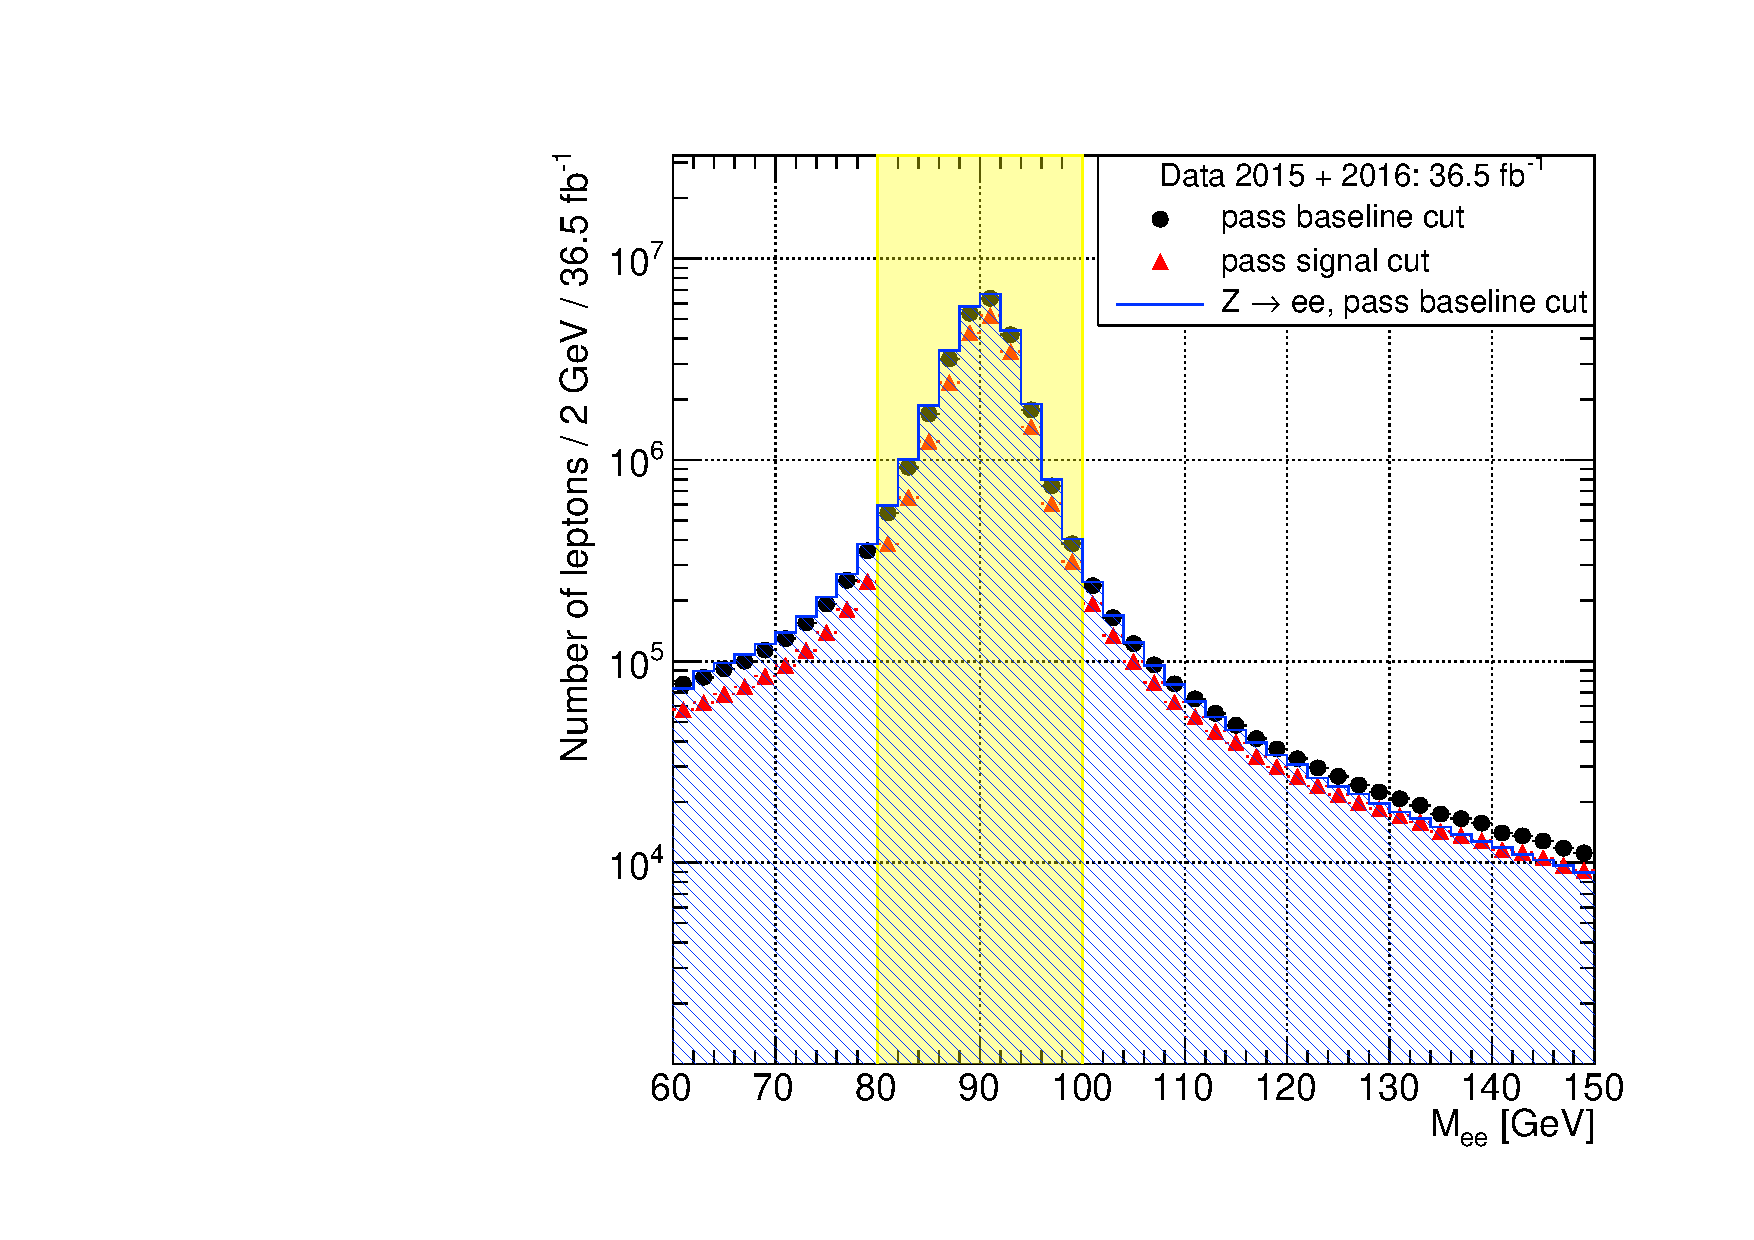
\includegraphics[width=\textwidth]{baseline_and_signal_mll_distribution_Mee.pdf}
\end{subfigure}
\begin{subfigure}[b]{0.45\textwidth}
	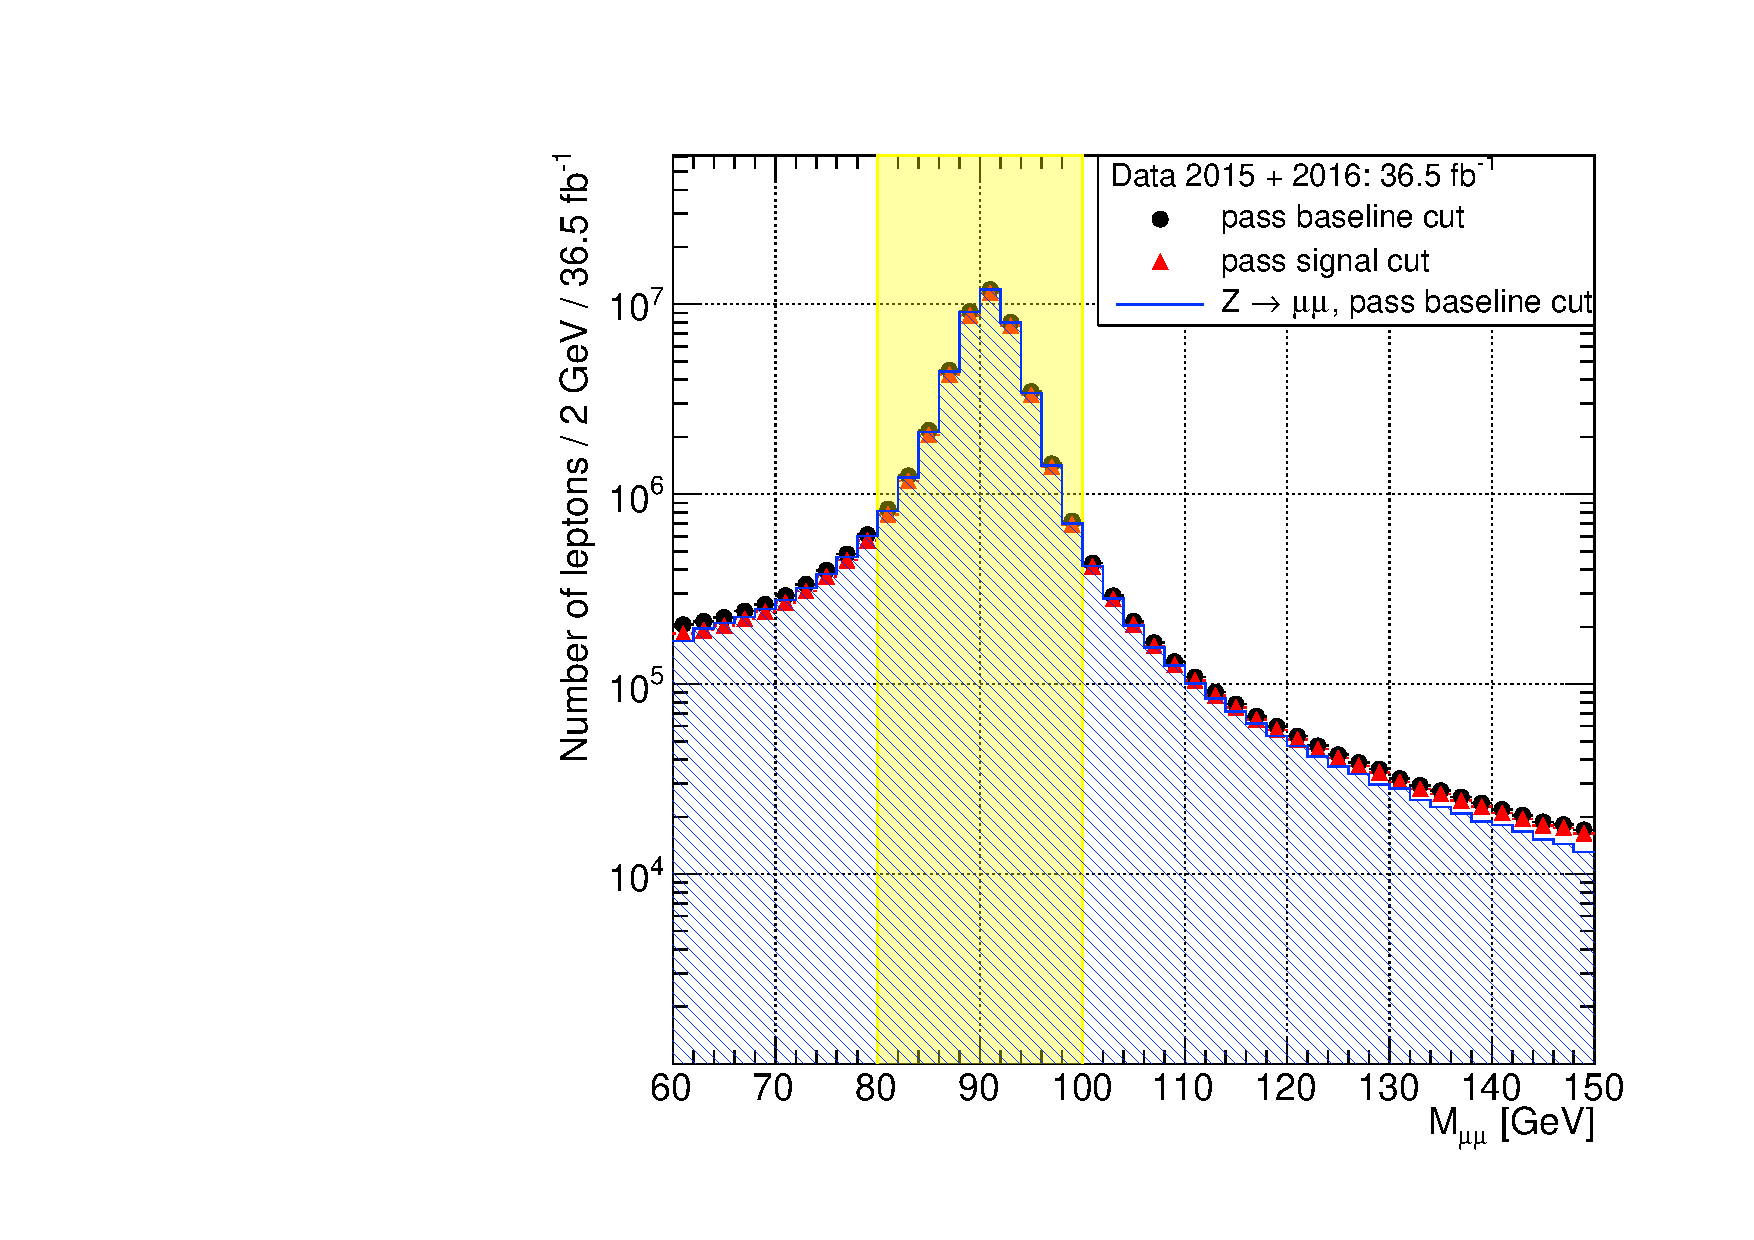
\includegraphics[width=\textwidth]{baseline_and_signal_mll_distribution_Mmumu.pdf}
\end{subfigure}
\caption{Invariant mass of opposite-sign same-flavor electrons (left) and muons (right), after the tag selection, 
where the probe satisfies the baseline requirements or the signal requirements.}
\label{fig:RLE_mll_distribution}
\end{figure}

A non-negligible background contamination in the electron channel affects measurements below $\pt=20~\GeV$. 
This contamination is taken into account in the measurement using a background template method inspired by the method used to measure reconstruction, identification, and 
isolation efficiencies documented in~\cite{ATLAS-CONF-2014-032}. 
This template is built from the tag-and-probe invariant mass distribution for baseline-level probe electrons that fail both tight identification
 and isolation requirements, smoothed by assuming an exponential shape whose parameters are determined by a fit in the interval $60<m_{ee}<120~\GeV$ excluding the $80<m_{ee}< 100~\GeV$ region. 
The background template is then normalized to the main tag-and-probe distribution in the background-dominated tail $120<m_{ee}<150~\GeV$. 
The estimated level of background goes up to $4\%$, reached for probe electrons with $\pt<15~\GeV$ and $|\eta|<0.8$. 

\begin{figure}[t!]
\centering
\begin{subfigure}{0.49\textwidth}
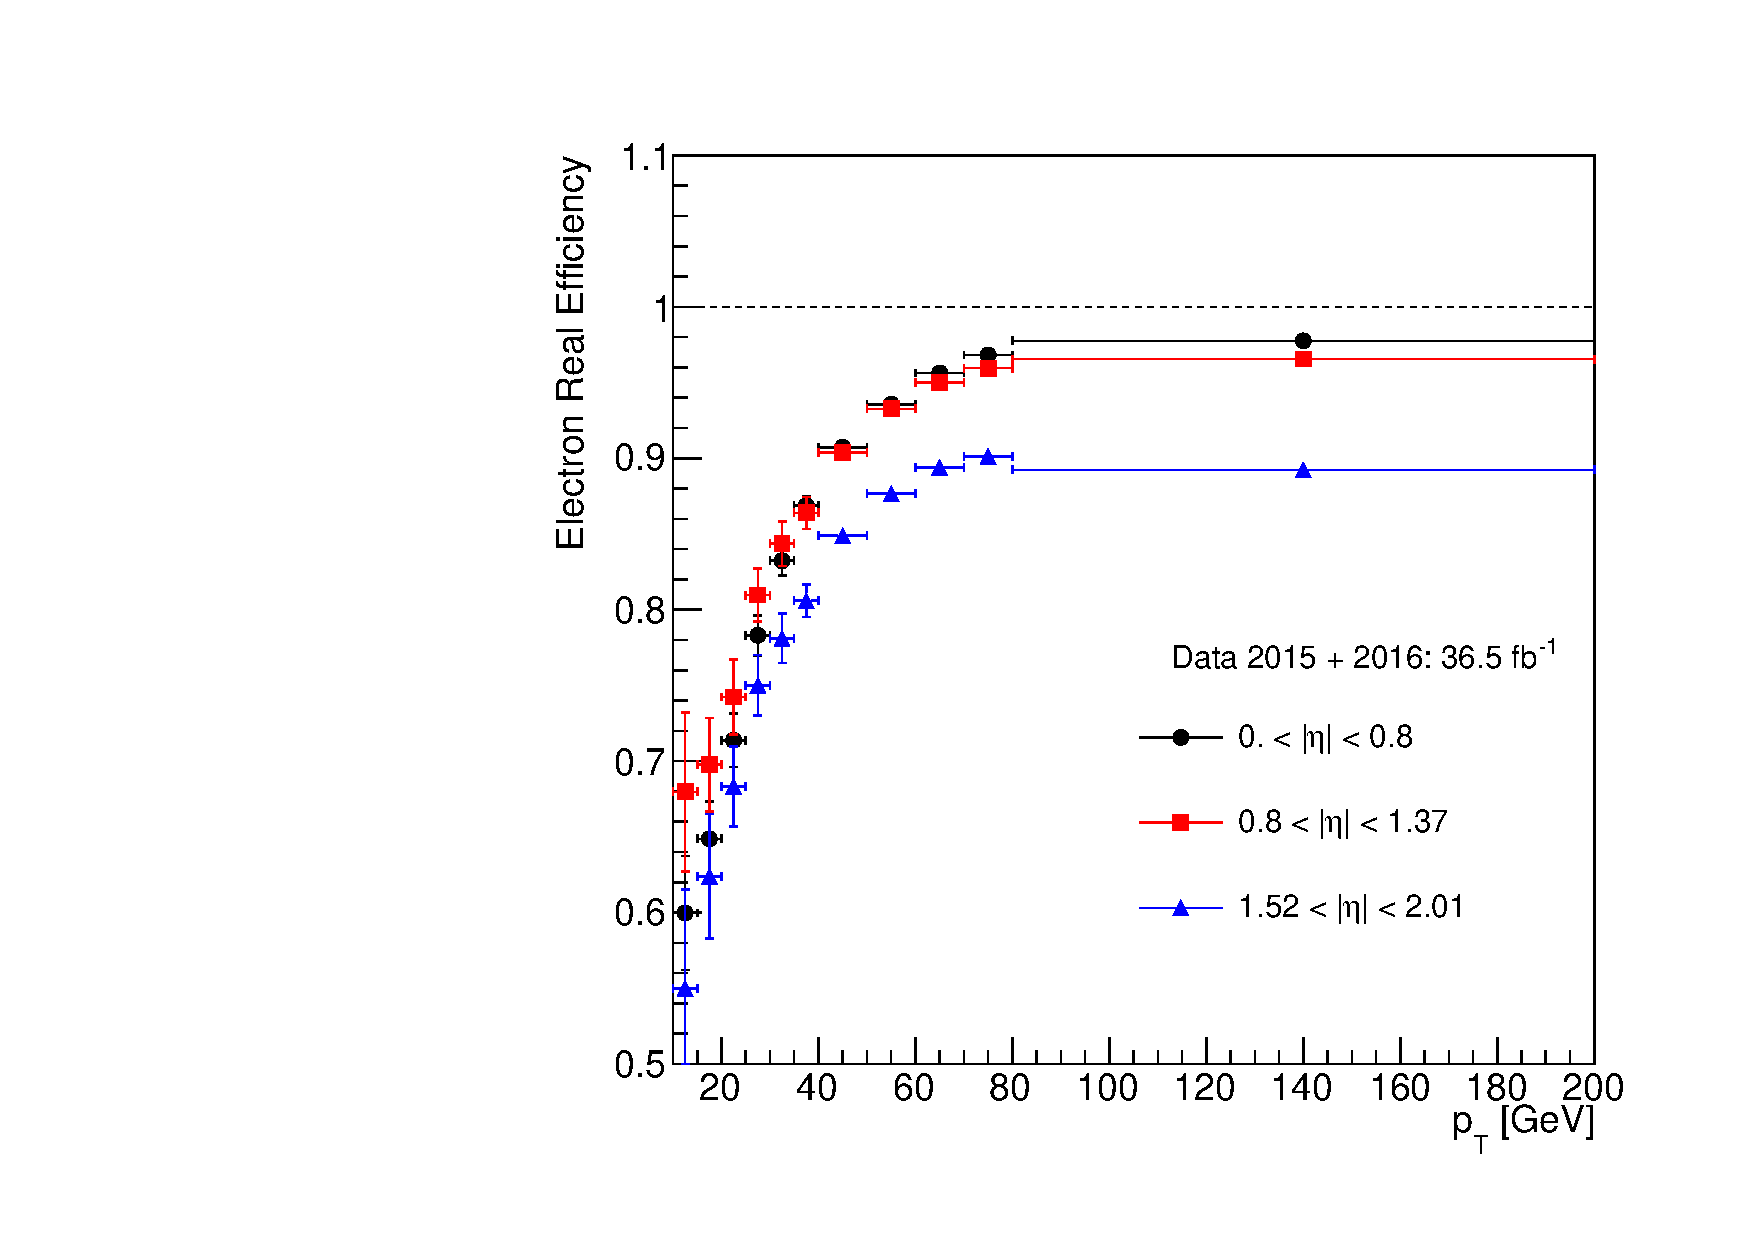
\includegraphics[width=\textwidth]{real_electron_efficiency_total_systematics.pdf}
\subcaption{Electrons}
\end{subfigure}
\begin{subfigure}{0.49\textwidth}
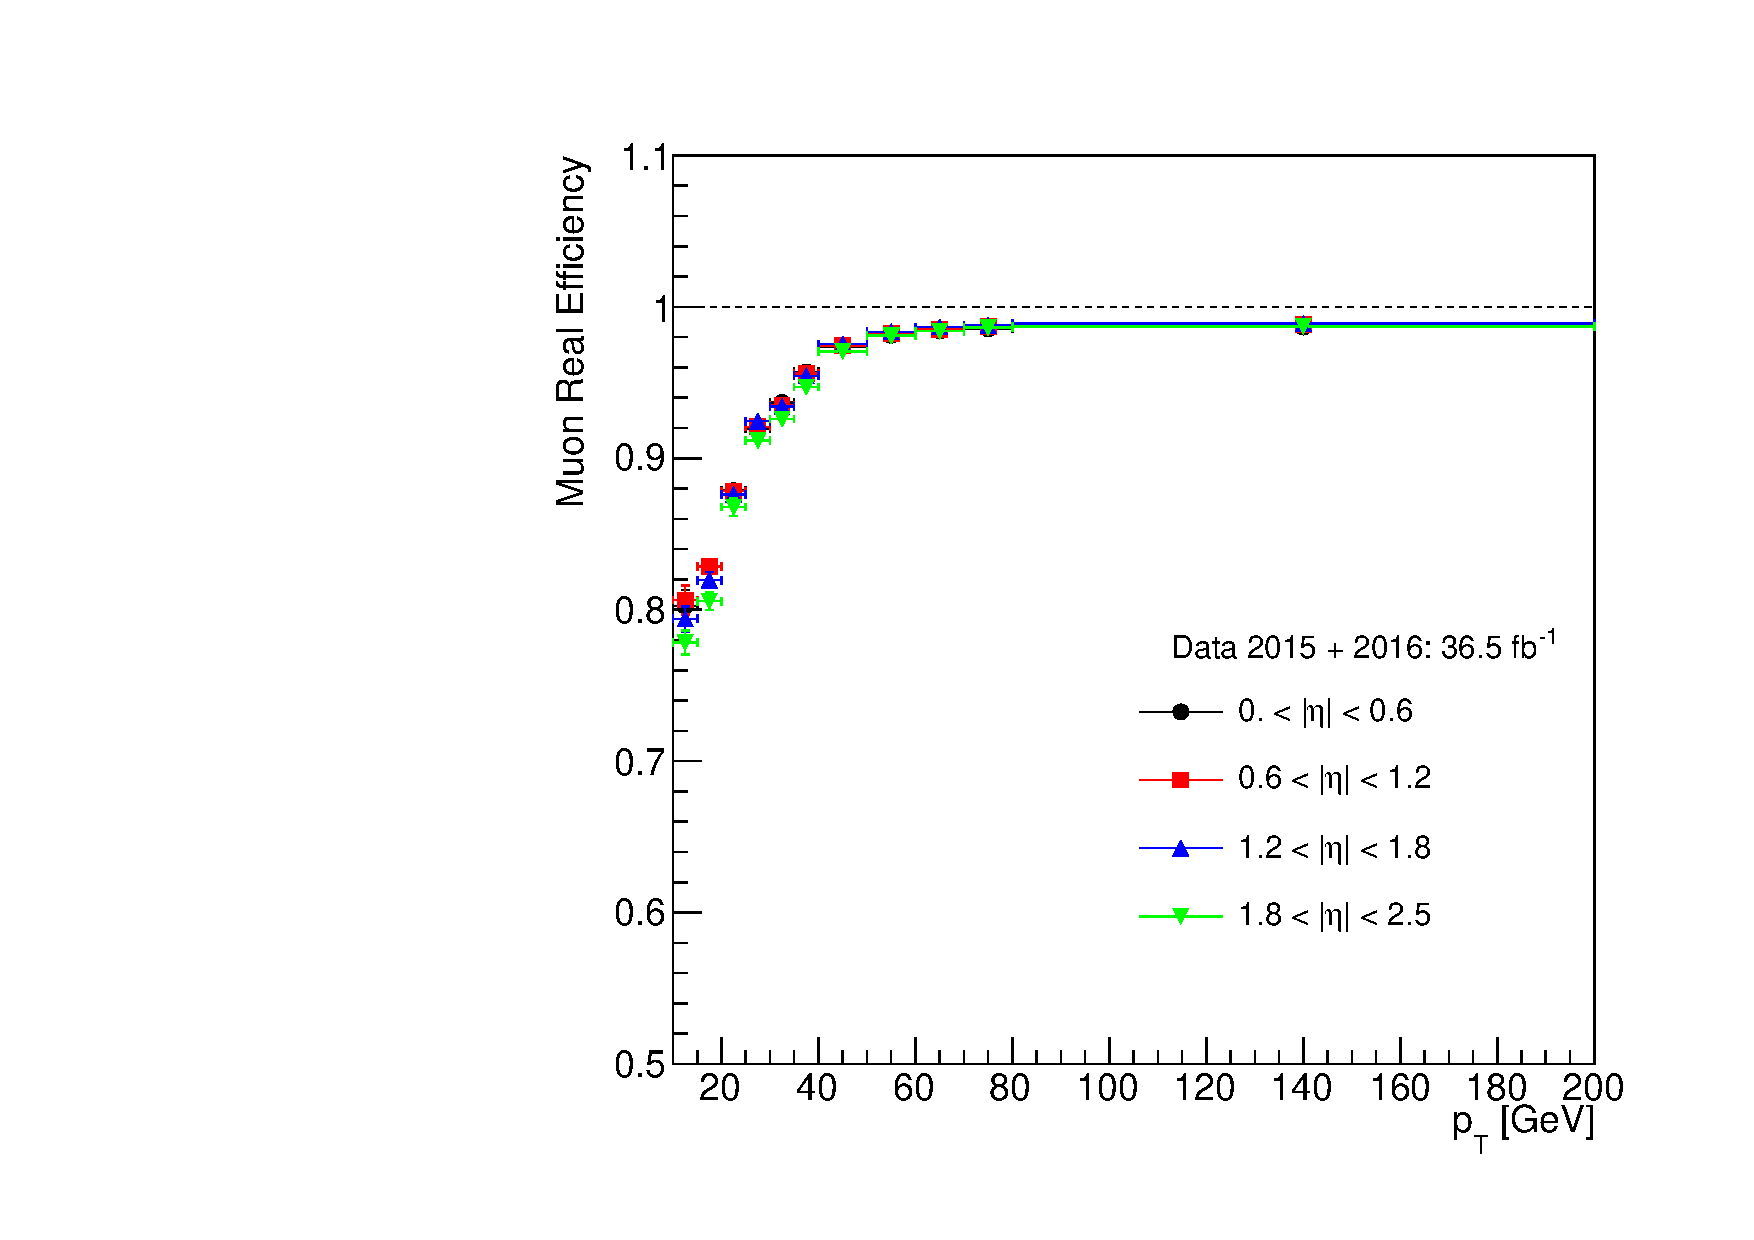
\includegraphics[width=\textwidth]{real_muon_efficiency_total_systematics.pdf}
\subcaption{Muons}
\end{subfigure}
\caption{Baseline-to-signal efficiencies as a function of $\pt$ and $|\eta|$ for real electrons (left) and muons (right), measured in 2015+2016 data.
%The background subtraction is applied on the electron channel only.
The $|\eta|$ binning used in the electron case corresponds to the geometry of the electromagnetic calorimeter.
For muons a homogeneous $|\eta|$ binning is considered.
The error bars corresponds to the quadratic sum of the statistical and tag-and-probe measurement systematic uncertainties.}
\label{fig:prompt_leptons_eff}
\end{figure}

The efficiency is measured as a function of \pt\ and $\eta$, and the results are presented in Fig~\ref{fig:prompt_leptons_eff} for electrons and muons. 
The background subtraction is applied on the electron channel only. 
The following systematic uncertainties are assigned to the measured efficiencies: 

\begin{itemize}
\item[$\bullet$] Background contamination: 27 variations of the tag-and-probe method are considered to assess the electron measurement systematics.
Three $m_{ee}$ windows and 9 variations of the background subtraction methods are considered.
The largest contribution to the systematics arises from the $m_{ee}$ window variation.
This is expected as the proportion of electrons affected by Brehmstrahlung depends on $m_{ee}$.
The resulting relative systematics vary from 6\% $\sim$ 12\% in the $10<\pt<15~\GeV$ region, 3\% to 6\% in the $15<\pt<20~\GeV$ region, 1\% to 3\% in the $20<\pt<40~\GeV$ region, and less than 1\% for $\pt >$ 40 \GeV.
The systematic uncertainties associated to the muon efficiencies measurement vary from 1\% to 1.3\% in the $10<\pt<15~\GeV$ region and less then 1\% for $\pt >$ 15 \GeV. 
\item[$\bullet$] Trigger: a systematic uncertainty accounting for a potential bias at trigger level is considered and it varies between 0 and 4\%, depending on the \pt range.
\item[$\bullet$] Extrapolation to busy environments: efficiencies are typically lower in such environments due to the proximity of jets and leptons; 
an uncertainty is assigned by comparing efficiencies in simulated $Z\to\ell\ell$ and $\gluino\to\ttbar\neut$ events, for $\Delta m(\gluino,\neut)>1~\TeV$ which represents an extreme case of final states with highly boosted top quarks. 
The uncertainty, taken as the difference in efficiencies, is parametrized as a function of \pt\ and $\Delta R$ (the angular distance between the lepton and the closest jet). 
\end{itemize}
%The resulting systematic uncertainties are summarized in Table~\ref{tab:RLE_systematics_bkg} and Table~\ref{tab:RLE_systematics_busy}. 
The resulting systematic uncertainties are summarized in Table~\ref{tab:RLE_systematics_all} and Table~\ref{tab:RLE_systematics_busy}.


\begin{center}
\begin{table}
\resizebox{\textwidth}{!}{%
\begin{tabular}{cccc|cccc}
\hline
\hline
& \multicolumn{3}{c}{Electrons} & \multicolumn{3}{c}{Muons}\\
& $0<|\eta|<0.8$ & $0.8<|\eta|<1.37$ & $1.52<|\eta|<2.01$ & $0<|\eta|<0.6$ & $0.6<|\eta|<1.2$ & $1.2<|\eta|<1.8$ & $1.8<|\eta|<2.5$\\
\hline
10~\GeV $< p_{\text T} <$ 15~\GeV & 0.047 & 0.063 & 0.089 & 0.014 & 0.010 & 0.008 & 0.011\\
15~\GeV $< p_{\text T} <$ 20~\GeV & 0.027 & 0.042 & 0.062 & 0.005 & 0.006 & 0.008 & 0.011\\
20~\GeV $< p_{\text T} <$ 25~\GeV & 0.018 & 0.031 & 0.041 & 0.003 & 0.006 & 0.010 & 0.010\\
25~\GeV $< p_{\text T} <$ 30~\GeV & 0.029 & 0.024 & 0.027 & 0.011 & 0.015 & 0.022 & 0.019\\
30~\GeV $< p_{\text T} <$ 35~\GeV & 0.023 & 0.021 & 0.023 & 0.007 & 0.009 & 0.014 & 0.011\\
35~\GeV $< p_{\text T} <$ 40~\GeV & 0.014 & 0.018 & 0.018 & 0.004 & 0.004 & 0.006 & 0.006\\
40~\GeV $< p_{\text T} <$ 50~\GeV & 0.007 & 0.010 & 0.010 & 0.002 & 0.001 & 0.002 & 0.001\\
50~\GeV $< p_{\text T} <$ 60~\GeV & 0.008 & 0.010 & 0.010 & 0.001 & 0.001 & 0.001 & 0.001\\
60~\GeV $< p_{\text T} <$ 70~\GeV & 0.007 & 0.010 & 0.010 & 0.001 & 0.001 & 0.001 & 0.002\\
70~\GeV $< p_{\text T} <$ 80~\GeV & 0.008 & 0.011 & 0.012 & 0.002 & 0.001 & 0.001 & 0.002\\
80~\GeV $< p_{\text T} <$ 120~\GeV & 0.010 & 0.010 & 0.011 & 0.004 & 0.002 & 0.002 & 0.002\\
120~\GeV $< p_{\text T} <$ 150~\GeV & 0.005 & 0.005 & 0.011 & 0.006 & 0.005 & 0.005 & 0.005\\
150~\GeV $< p_{\text T} <$ 200~\GeV & 0.005 & 0.002 & 0.019 & 0.005 & 0.005 & 0.005 & 0.006\\
\hline
\hline
\end{tabular}
}
\caption{
Systematic uncertainties on the measured real lepton efficiency, separating sources affecting the measurement itself (background subtraction, trigger bias, and different methods). 
}
\label{tab:RLE_systematics_all}
\end{table}
\end{center}

\begin{center}
\begin{table}
\resizebox{\textwidth}{!}{%
\begin{tabular}{ccccccccccc}
\hline
\hline
\multicolumn{9}{c}{electrons (busy environments)}\\
\hline
$\Delta R(e, jet)$ & [0, 0.1] & [0.1, 0.15] & [0.15, 0.2] & [0.2, 0.3] & [0.3, 0.35] & [0.35, 0.4] & [0.4, 0.6] & [0.6, 4]\\
\hline
10~\GeV $< p_{\text T} <$ 20~\GeV & - & - & - & - & - & - & 25.31\% & 6.5\%\\
20~\GeV $< p_{\text T} <$ 30~\GeV & - & - & - & - & - & 73.37\% & 10.21\% & 0.37\%\\
30~\GeV $< p_{\text T} <$ 40~\GeV & - & - & - & 97.71\% & 48.22\% & 15.54\% & 7.29\% & 0.58\%\\
40~\GeV $< p_{\text T} <$ 50~\GeV & - & - & - & 52.81\% & 22.80\% & 16.73\% & 7.68\% & 1.10\%\\
50~\GeV $< p_{\text T} <$ 60~\GeV & - & - & - & 29.96\% & 21.49\% & 20.23\% & 6.99\% & 2.78\%\\
60~\GeV $< p_{\text T} <$ 80~\GeV & - & - & 55.89\% & 24.31\% & 17.40\% & 24.77\% & 6.20\% & 2.87\%\\
80~\GeV $< p_{\text T} <$ 150~\GeV & - & 57.52\% & 30.24\% & 16.45\% & 12.73\% & 20.92\% & 4.44\% & 2.73\%\\
150~\GeV $< p_{\text T} <$ 200~\GeV & 88.54\% & 40.16\% & 19.34\% & 8.45\% & 14.66\% & 16.57\% & 2.57\% & 1.90\%\\
\hline
\hline
%\end{tabular}
%}
%\resizebox{\textwidth}{!}{%
%\begin{tabular}{ccccccccccc}
%\hline
%\hline
\multicolumn{9}{c}{muons (busy environments)}\\
\hline
$\Delta R(\mu, jet)$ & [0, 0.1] & [0.1, 0.15] & [0.15, 0.2] & [0.2, 0.3] & [0.3, 0.35] & [0.35, 0.4] & [0.4, 0.6] & [0.6, 4]\\
\hline
10~\GeV $< p_{\text T} <$ 20~\GeV & - & - & - & - & - & - & 33.59\% & 5.18\%\\
20~\GeV $< p_{\text T} <$ 30~\GeV & - & - & - & - & - & 82.34\% & 22.27\% & 3.39\%\\
30~\GeV $< p_{\text T} <$ 40~\GeV & - & - & -  & 98.54\% & 56.36\% & 31.89\% & 14.22\% & 2.24\%\\
40~\GeV $< p_{\text T} <$ 50~\GeV & - & - & - & 53.10\% & 21.33\% & 13.90\% & 6.81\% & 1.45\%\\
50~\GeV $< p_{\text T} <$ 60~\GeV & - & - & - & 24.98\% & 13.72\% & 9.62\% & 3.83\% & 0.79\%\\
60~\GeV $< p_{\text T} <$ 80~\GeV & - & - & 44.41\% & 13.75\% & 6.14\% & 4.76\% & 2.04\% & 0.15\%\\
80~\GeV $< p_{\text T} <$ 150~\GeV & - & 29.94\% & 7.14\% & 3.16\% & 1.30\% & 1.04\% & 0.07\% & 0.57\%\\
150~\GeV $< p_{\text T} <$ 200~\GeV & 82.26\% & 4.14\% & 1.02\% & 0.17\% & 0.29\% & 0.62\% & 1.02\% & 1.13\%\\
\hline
\hline
\end{tabular}
}
\caption{
Systematic uncertainties on the measured real lepton efficiency, due to the extrapolation to busy environments using $\gluino \to \ttbar \tilde{\chi_1^0}$ events. 
}
\label{tab:RLE_systematics_busy}
\end{table}
\end{center}


\subsection{MC Template Method}
As discussed in Section~\ref{sec:fake.mct}, the MC template method is
 a simulation-based method that provides an alternative estimate of the reducible backgrounds affecting the analysis.
It relies on the correct modelling of FNP leptons and charge-flipped electron kinematics in $\ttbar$ 
and $V$+jets.
FNP leptons are classified in four categories, namely electrons and muons coming 
from $b$ and light-quark jets. Normalisation factors for each of the five sources (including photon conversions) are computed to match the observed data 
in dedicated control regions. The fifth category is events with prompt electrons that have a charge mis-measurement 
(charge flip, electron heavy flavor (EL HF), 
muon heavy flavor (MU HF), 
electron light flavor (EL LF), 
muon light flavor (MU LF)).
Six non-overlapping control regions are defined by the presence of $b$-jets and by the flavors of the same sign lepton pair in the event:
\begin{itemize}
\item CR0b: events without $b$-jets in $ee$, $e\mu$, and $\mu\mu$ channels.
\item CR1b: events with at least one $b$-jet in $ee$, $e\mu$, and $\mu\mu$ channels.
\end{itemize}
All the selected events contain two or more same-sign signal leptons and \\$\met >40~\GeV$ and 2 or more jets. 
Events satisfying the signal regions requirements are excluded from the control regions. 
The purpose of the \met requirement is to remove multi-jet events that have two or more FNP leptons and tend to have low \met. 
The six distributions are chosen for variables that provide the best separation between processes with prompt leptons and processes with 
fake leptons and charge flip and are shown 
before and after the fit in Figures \ref{f:prefit_CR0b}-\ref{f:prefit_CR1b} and Figures \ref{f:postfit_CR0b}-\ref{f:postfit_CR1b}, 
respectively. 
The multipliers obtained after the minimization of the negative log likelihood were given 
in Tables \ref{t:fake_factors_powheg} and \ref{t:fake_factors_sherpa}.
The tables represent the correction factors obtained from the fit upon using two different parton showers, \POWHEGBOX+Pythia and \SHERPA
for the processes that lead to non-prompt leptons and charge flips.
The goal of varying the parton shower is to access the dependence of the fake and charge flip estimates on the choice of the 
parton shower. 

The MC template method is validated by looking at the agreement 
between observed data and prediction as shown in Figures~\ref{fig:bkg.val.met}.
In the MC template method, the systematic uncertainty is obtained by
changing the generator from \POWHEGBOX+Pythia to \SHERPA and propagating uncertainties from the control region fit to the global
normalization scale factors applied to the MC samples. 
The uncertainties in these scale factors are in the range 75--80\%,
depending on the SRs.
In practice, only \ttbar contributes to the SRs and the final yields with systematic uncertainties from 
fit uncertainty, theory uncertainties on \ttbar, and comparison of different showers (Pythia and Sherpa) are shown in Table \ref{tab:fakes_mcglobal}.
This table also shows a global correction factor derived by taking the ratio of the weighted \ttbar to raw MC \ttbar with
a global uncertainty that includes all systematic uncertainties used to obtain the final estimate. 

\begin{table}[!htb]
\centering
\resizebox{\textwidth}{!}{
\begin{tabular}{|c||c|c|c||}\hline
Region &              MC Template method  & Global correction & Shower systematic \\
\hline
Rpc2L0bH & $1.00 \pm 0.96 \pm 0.81$ & $2.80 \pm 2.10$ & 74\% \\
Rpc2L0bS & $1.68 \pm 1.02 \pm 1.26$ & $2.89 \pm 1.97$ & 65\% \\
Rpc2L1bH & $2.07 \pm 0.63 \pm 1.56$ & $1.22 \pm 1.14$ & 34\% \\
Rpc2L1bS & $2.33 \pm 1.17 \pm 2.10$ & $1.83 \pm 1.42$ & 81\% \\
Rpc2L2bH & $<0.5$ & $0 \pm 0$ & 0\% \\
Rpc2L2bS & $0.41 \pm 0.33 \pm 0.45$ & $1.47 \pm 1.12$ & 73\% \\
Rpc2Lsoft1b & $2.48 \pm 1.32 \pm 1.86$ & $1.59 \pm 1.31$ & 68\% \\
Rpc2Lsoft2b & $1.66 \pm 0.66 \pm 1.28$ & $1.72 \pm 1.29$ & 54\% \\
Rpc3L0bH & $<0.5$ & $0 \pm 0$ & 0\% \\
Rpc3L0bS & $0.21 \pm 0.15 \pm 0.16$ & $2.90 \pm 2.20$ & 71\% \\
Rpc3L1bH & $0.42 \pm 0.29 \pm 0.32$ & $1.59 \pm 1.25$ & 59\% \\
Rpc3L1bS & $3.55 \pm 1.80 \pm 2.76$ & $1.76 \pm 1.32$ & 67\% \\
Rpc3LSS1b & $0.90 \pm 0.14 \pm 0.69$ & $2.34 \pm 1.44$ & 56\% \\
\hline
\hline
\end{tabular}
}
\caption{Expected yields for background processes with fake leptons,
in the signal regions with a global correction factor that represents the ratio of weighted \ttbar to raw MC \ttbar with
a global uncertainty that includes: fit uncertainty, theory uncertainties on \ttbar, comparison of different showers. 
The fraction of the systematic uncertainty from the comparison between two showers (Pythia and Sherpa) is also shown.
}
\label{tab:fakes_mcglobal}
\end{table}



\subsection{Background processes with charge-flipped electrons}
The lepton charge mis-measurement commonly referred to as ``charge flip'', 
is an experimental background strongly associated to analyses relying on same-sign lepton final states. 
In those events, the electric charge of one of the two leptons forming an opposite-sign (OS) pair, 
coming from an abundant SM process ($pp\to Z$, \ttbar, $W^+W^-$\ldots), 
is mis-identified leading to a much rarer same-sign (SS) pair event.
In most cases, the source of such a mis-identification 
is the creation of additional close-by tracks $e^\pm\to e^\pm\gamma\to e^\pm e^\pm e^\mp$ 
via Brehmstrahlung of the original electron when interacting with the material of the inner tracker. 
If one of the secondary electron tracks is subsequently preferred to the original track in the reconstruction of the electron candidate, 
the charge assigned to the electron might be incorrect, leading to a charge-flip event. 
Errors on the track charge assignment itself may occur as well, but they are much rarer. 
In the case of muons, charge-flip is essentially negligible due to the much smaller interaction cross-section with matter, 
and the requirement of identical charges to be measured for the inner tracker and muon spectrometer tracks. 

A purely data-driven method is used to estimate event yields for the 
electron charge-flip background. 
Assuming that the electron charge flip rates $\xi(\eta,\pt)$ are known, 
a simple way to predict these yields is to select events with pairs of opposite-sign leptons in data and assign them a weight:

\begin{align}
w_\text{flip} = \xi_1(1-\xi_2) + (1-\xi_1)\xi_2
\label{eqn:chargeflip_weight}
\end{align}
where $\xi_{(i)}=0$ for muons.

The advantages of this method are a good statistical precision since the charge flip rate is quite small, 
and the absence of dependency to the simulation and related uncertainties. 
Obviously, it requires a precise measurement of the rates, which is described in this section. 
An inconvenience of this approach is that the reconstructed momentum for charge-flipped electrons  
tends to be negatively biased (too low by a few GeV), 
since such important Brehmstrahlung topologies represent only 
a very small fraction of the cases used to tune electron energy calibration. 
Simply re-weighting electrons from opposite-sign lepton pairs therefore does not predict correctly 
the charge-flip background shape for variables very sensitive to the electron momentum, for example the $m_{ee}$ line-shape. 
However, the kinematic range and variables used in the analysis are not
sensitive to this effect and can safely be neglected.

For the nominal (tight) estimate of the charge-flip background contributions, only events with exactly two OS signal electrons are considered. 
Corrections in the fake lepton estimate however require estimating as well charge-flip contributions for selections involving 
baseline electrons failing signal requirements; 
for that reason, the charge-flip (loose) rate is measured for these two categories of electrons. 

\subsection*{Methodology}
\label{subsec:chargeflip_method}

\begin{figure}[t!]
\centering
\begin{subfigure}[b]{0.45\textwidth}
	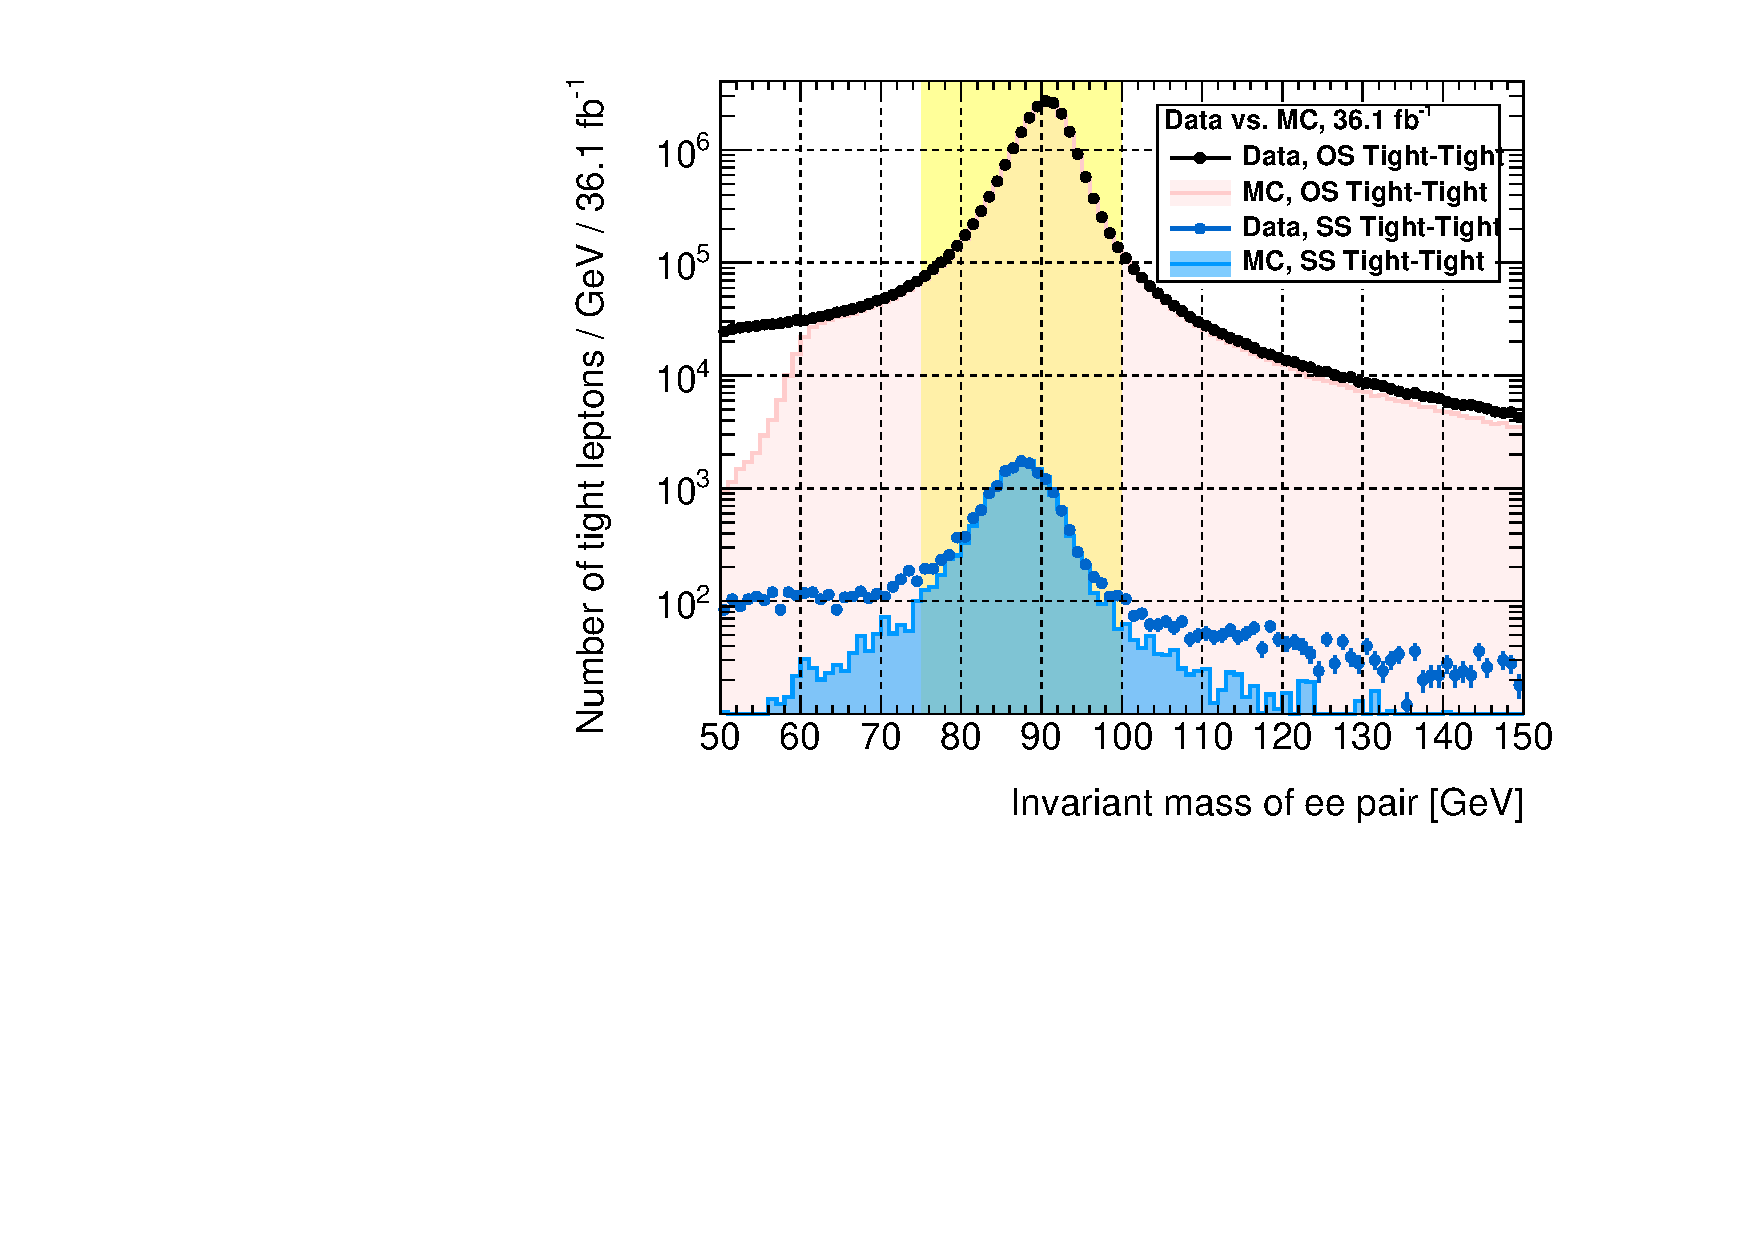
\includegraphics[width=\textwidth]{Data_vs_MC_Pass_EL}
\end{subfigure}
\begin{subfigure}[b]{0.45\textwidth}
	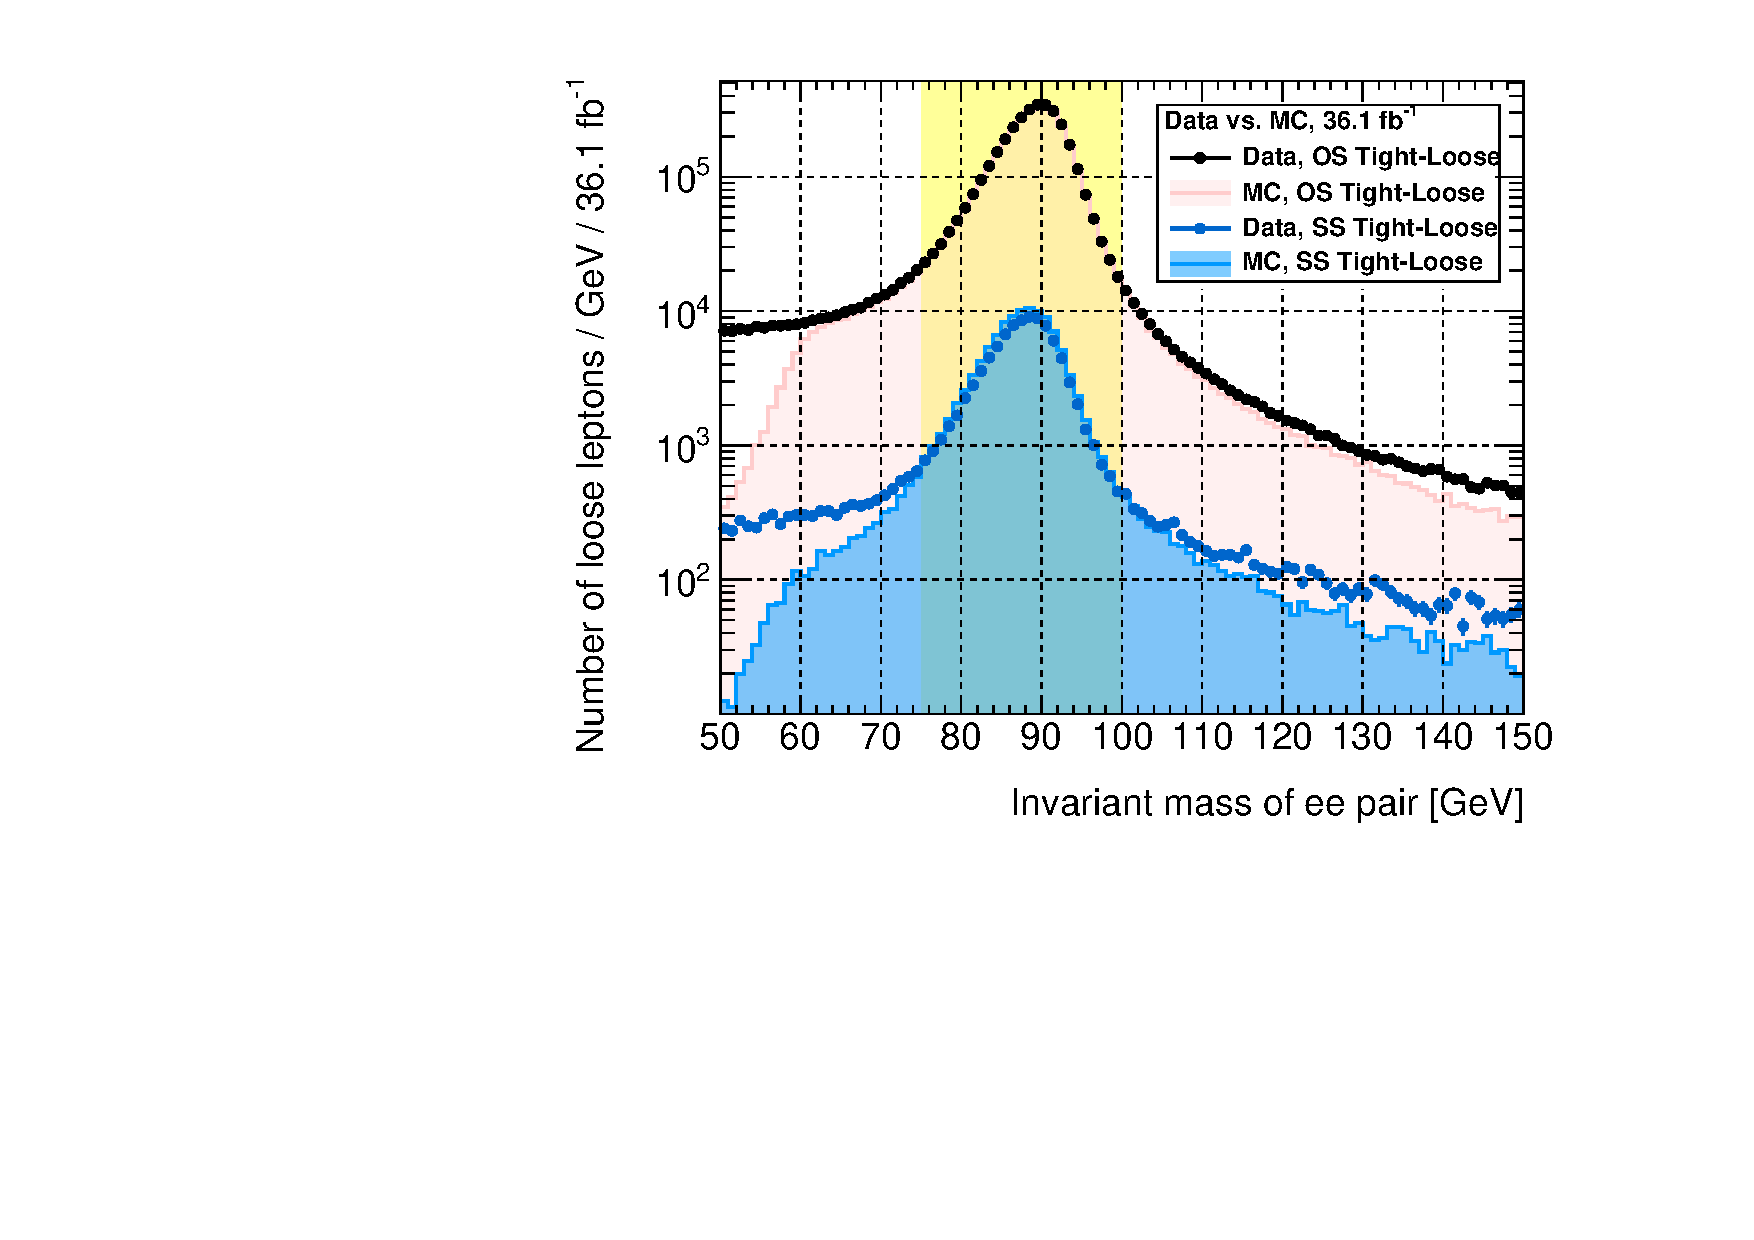
\includegraphics[width=\textwidth]{Data_vs_MC_Fail_EL}
\end{subfigure}
\caption{Invariant mass of opposite- and same-sign electron pairs, 
when both electrons satisfy signal requirements (left) or one of them fails them (right). Drell-Yan MC samples are not included, thus the drop in the MC distributions (light magenta filled area).}
\label{fig:chargeflip_mee}
\end{figure}

Charge-flip rates are measured in data relying on a clean $Z\to ee$ sample ($75<m_{ee}<100~\GeV$), 
in which the rates can be determined from the relative proportions of OS and SS electron pairs. 
Figure~\ref{fig:chargeflip_mee} illustrates this event selection. 
The rates are measured as function of $\eta$ and \pt, to follow their dependency to the distribution of material in the detector, 
the Brehmstrahlung emission rate, and the track curvature. 
Because of this binned measurements, and because the two electrons in a given pair generally have different kinematic properties, 
it has been found that the most efficient and least biased use of the available statistics 
is obtained by simultaneously extracting the rates in all bins via the maximization of the likelihood function describing the 
Poisson-expected yields of SS pairs: 

\begin{equation}
\begin{aligned}
{} & L(\{N^\text{SS,obs}_\varpi\}|\{\xi(\eta,\pt)\}) 
= \\
& \prod_{\varpi} \mathcal P\left(N^\text{SS,obs}_\varpi|w_\text{flip}(\xi(\eta_1,p_{\mathrm{T},1}),\xi(\eta_2,p_{\mathrm{T},2}))\times N^\text{OS+SS,obs}_\varpi\right)
\label{eqn:chargeflip_likelihood}
\end{aligned}
\end{equation}
with $\varpi=(\eta_1,p_{\mathrm{T},1},\eta_2,p_{\mathrm{T},2})$ indexing bins, where (arbitrarily) $p_{\mathrm{T},1}>p_{\mathrm{T},2}$; 
the expression of $w_\text{flip}$ is given by~(\ref{eqn:chargeflip_weight}). 
Statistical uncertainties on the extracted charge-flip rates are obtained (in a standard way) from the likelihood's numerically-computed Hessian matrix. 

In the nominal charge-flip measurement, the two electrons are required to satisfy signal requirements. 
To measure charge-flip rates for baseline electrons failing signal (noted $\bar\xi$ below), 
pairs with only one signal electron are used; 
this provides larger statistics than applying~(\ref{eqn:chargeflip_likelihood}) to electrons pairs where both fail the signal cuts. 
However, the expression of the likelihood has to be adapted due to the induced asymmetry between the two electrons forming the pair: 
%\small{
\begin{equation}
\begin{aligned}
{} & L(\{N^\text{SS,obs}_\varpi\}|\{\xi(\eta_1,p_{\mathrm{T},1})\},\{\bar\xi(\eta_2,p_{\mathrm{T},2})\}) 
= \\
& \prod_{\varpi} \mathcal P\left(N^\text{SS,obs}_\varpi|w_\text{flip}(\xi(\eta_1,p_{\mathrm{T},1}),\bar\xi(\eta_2,p_{\mathrm{T},2}))\times N^\text{OS+SS,obs}_\varpi\right)
\label{eqn:chargeflip_likelihood_loose}
\end{aligned}%}
\end{equation}
where this time $(\eta_1,p_{\mathrm{T},1})$ corresponds to the signal electron. 
Using the same $\eta$ and \pt binning for both measurements, 
the number of free variables in the maximization of~(\ref{eqn:chargeflip_likelihood_loose}) 
-- as well as the number of terms in the product forming $L$ -- 
is twice as large as the nominal case~(\ref{eqn:chargeflip_likelihood}). 
In fact, a by-product of the maximization of~(\ref{eqn:chargeflip_likelihood_loose}) is another determination of the charge-flip rates for signal electrons, 
although with a more limited precision than obtained in the nominal measurement~(\ref{eqn:chargeflip_likelihood}).

Background subtraction is performed through a simple linear extrapolation of the invariant mass distribution sidebands; 
it matters mostly for low \pt in the nominal measurement, 
and for the additional measurement with baseline electrons failing signal requirements, where the level of background is larger. 

\subsection*{Measured rates}
\label{subsec:chargeflip_rates}

\begin{figure}[htb!]
\centering
\begin{subfigure}[b]{0.49\textwidth}
	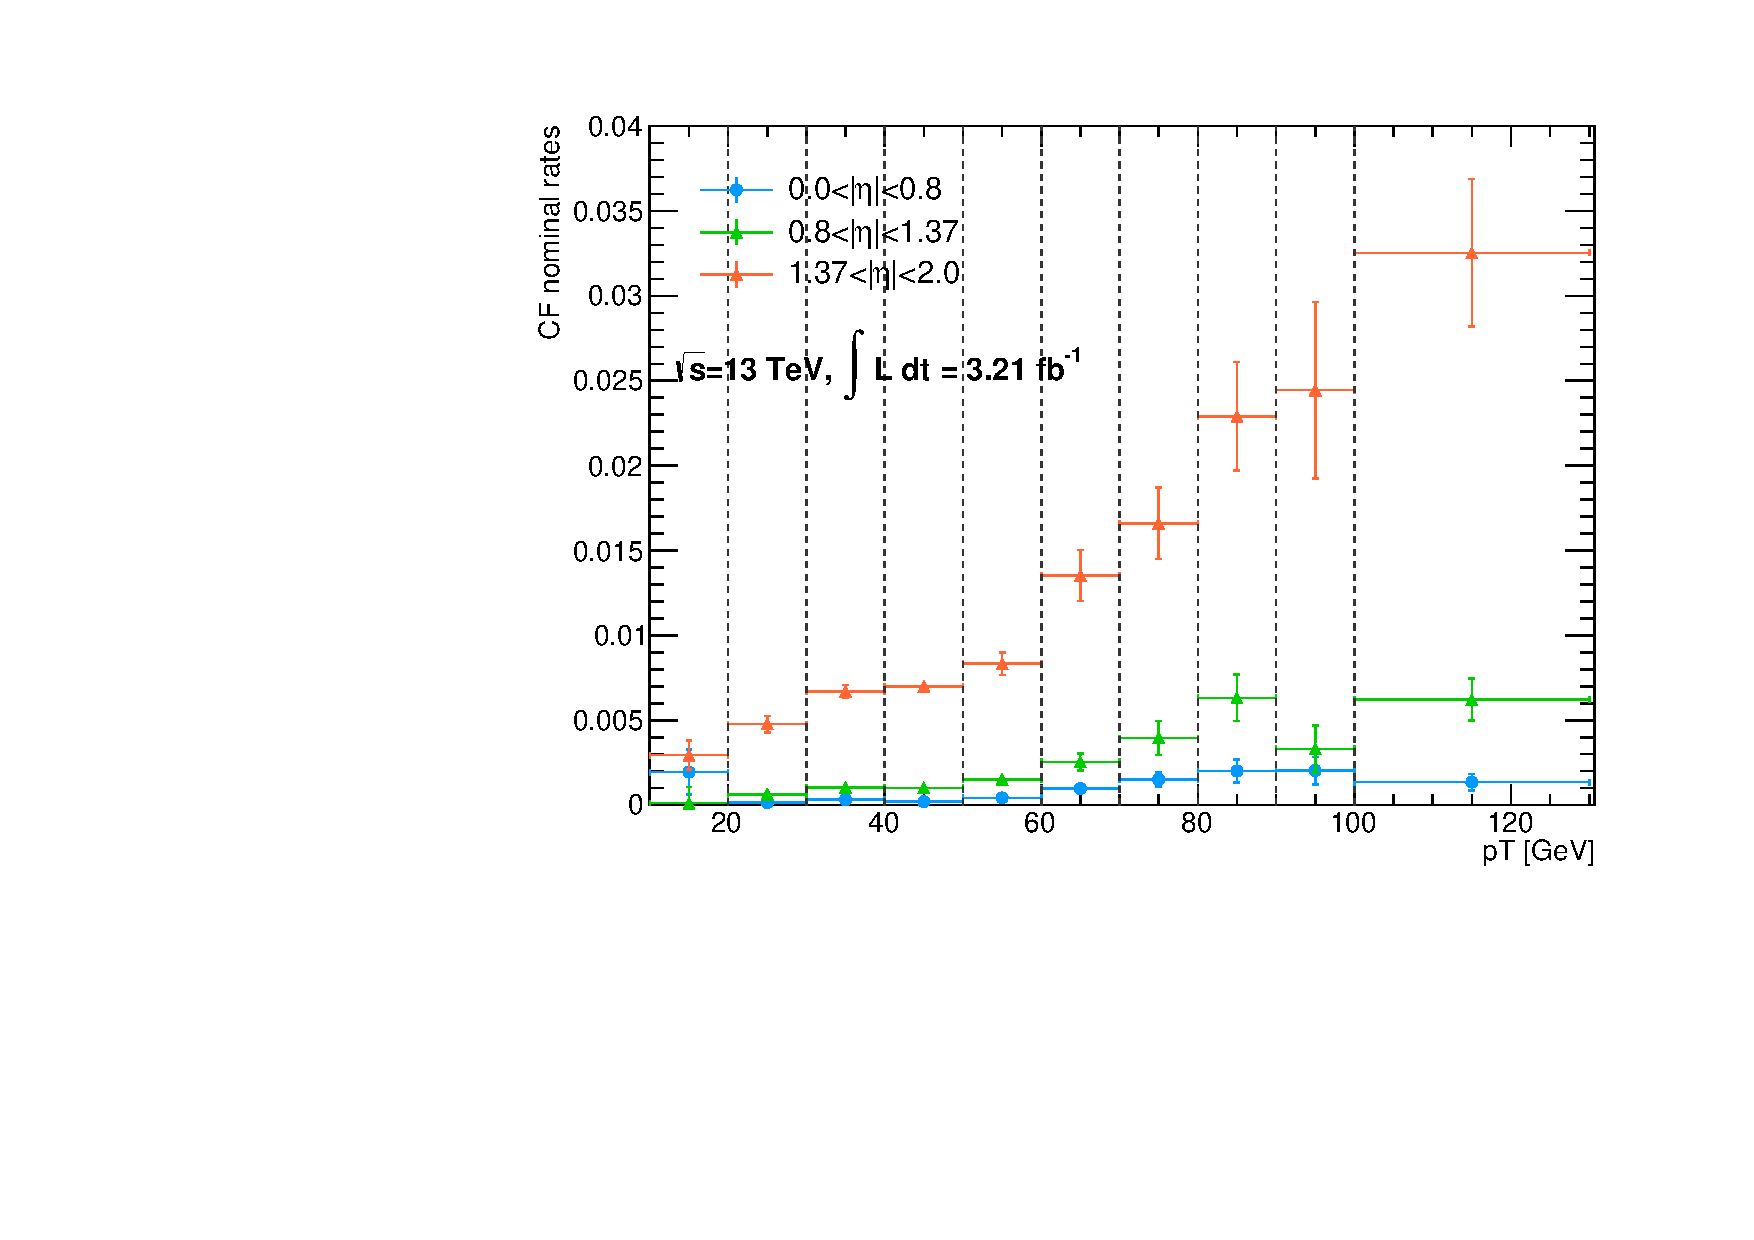
\includegraphics[width=\textwidth]{CFratesVSpt_data15}
	\caption{Data, signal electrons}\label{fig:Chflip_nominalData}
\end{subfigure}
\begin{subfigure}[b]{0.49\textwidth}
	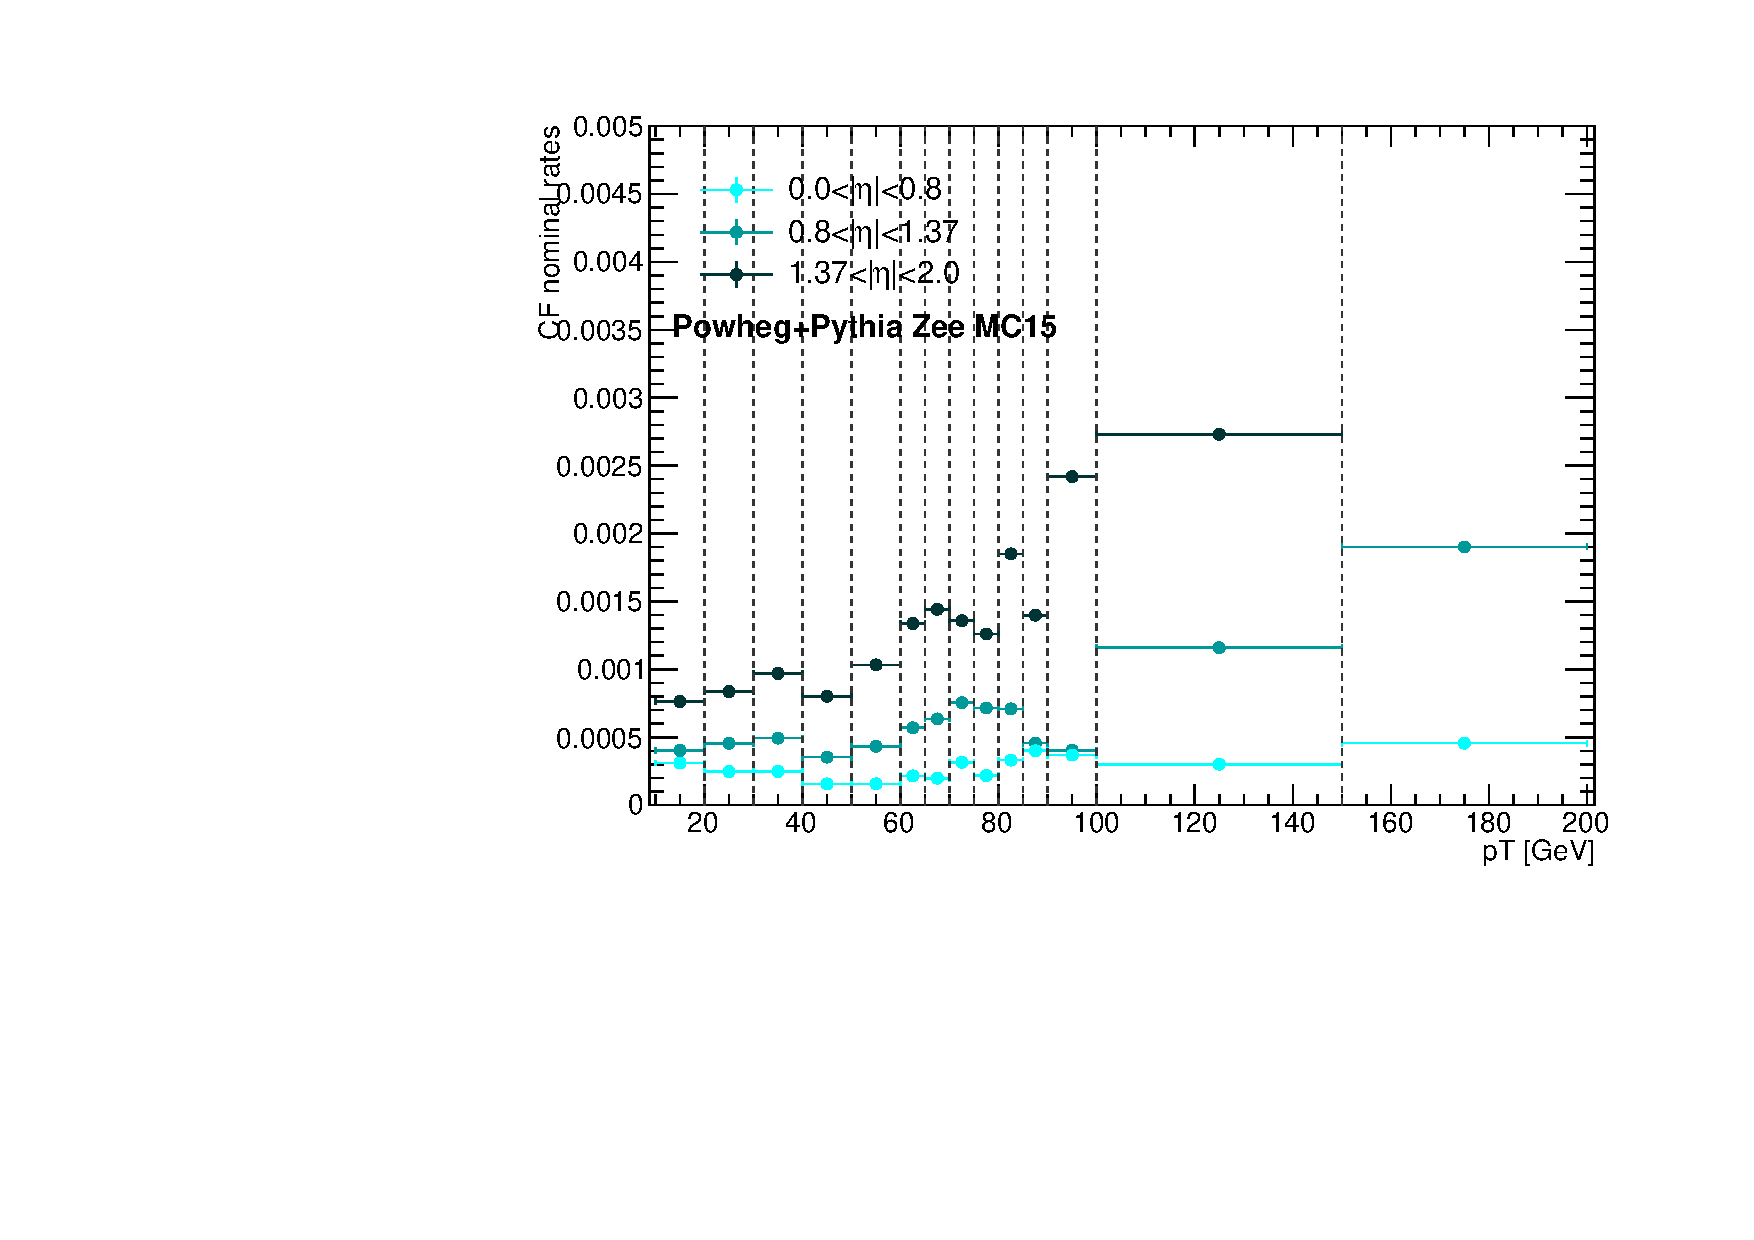
\includegraphics[width=\textwidth]{CFratesVSpt_MC15}
	\caption{MC, signal electrons}\label{fig:Chflip_nominalMC}
\end{subfigure}
\begin{subfigure}[b]{0.49\textwidth}
	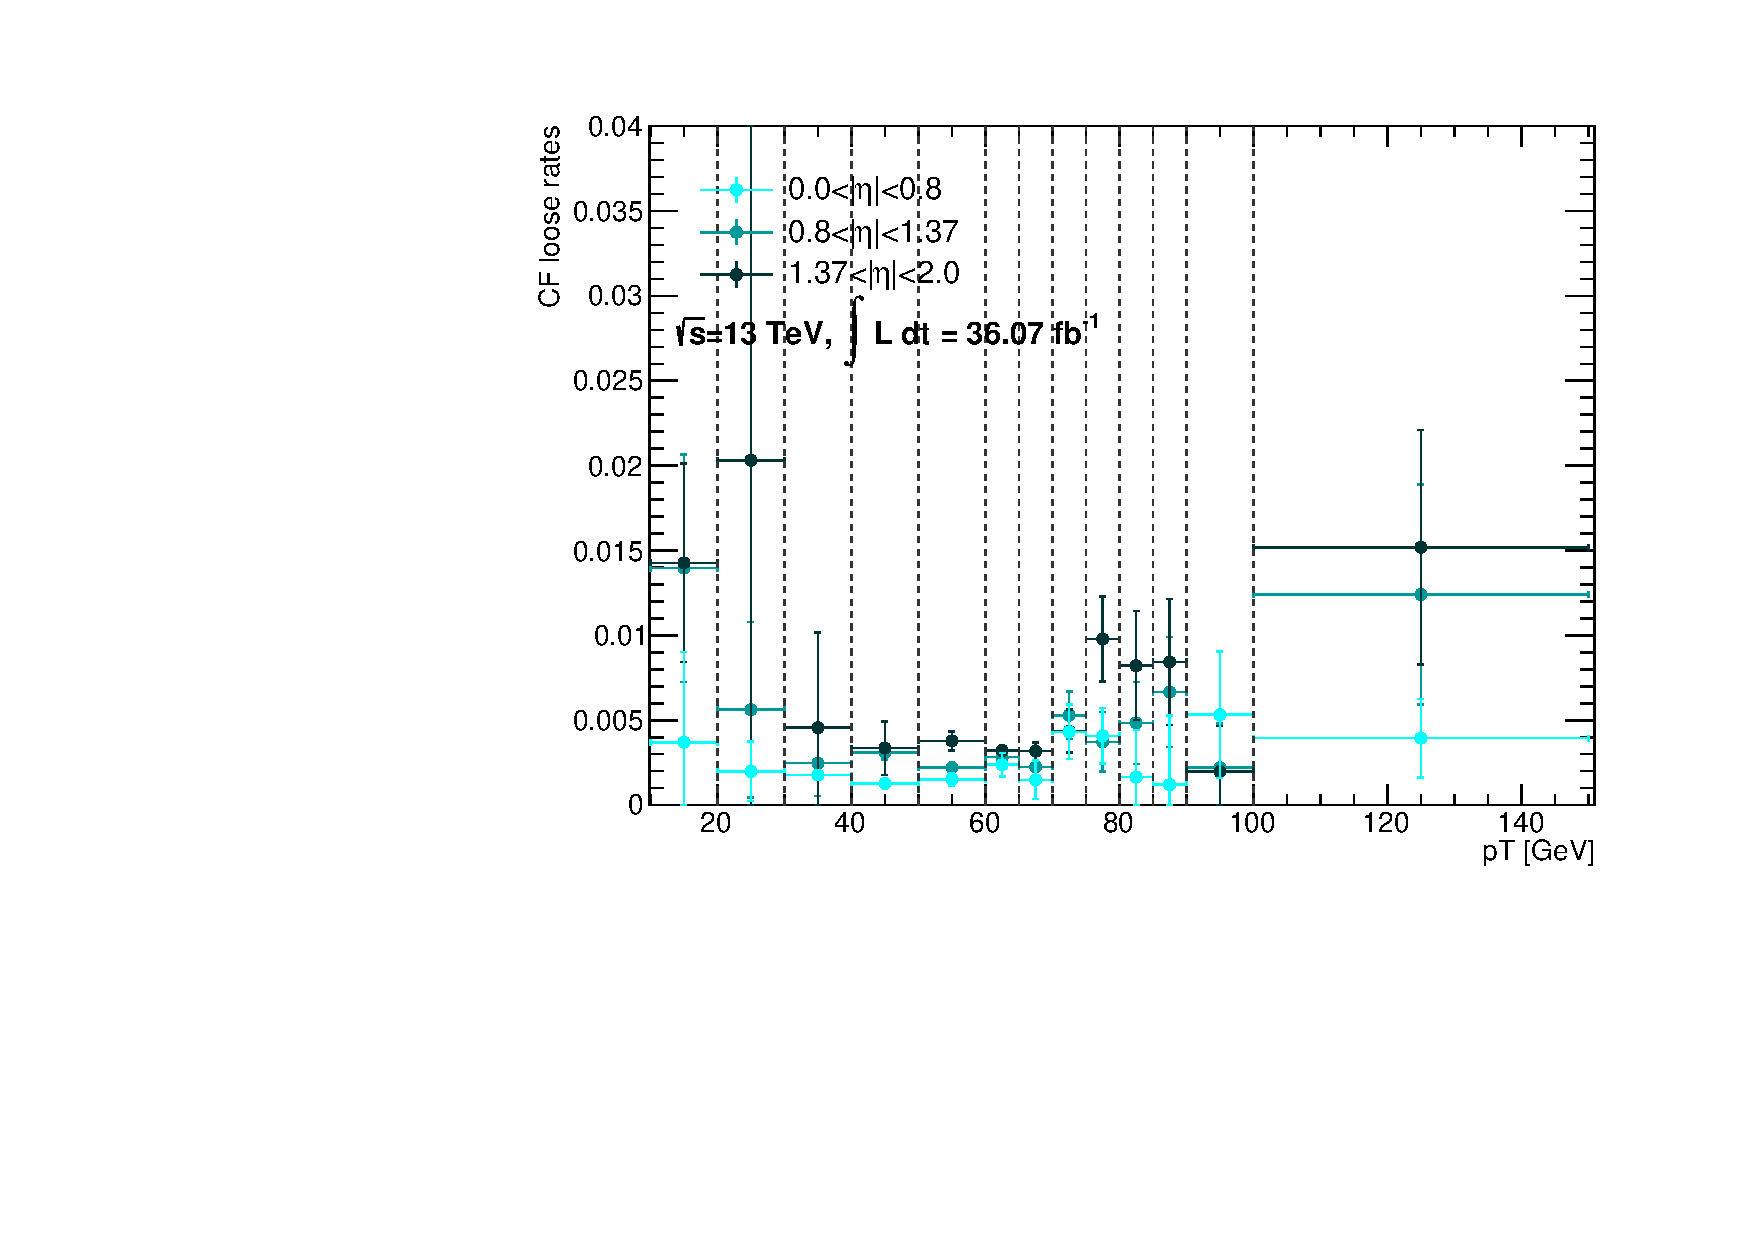
\includegraphics[width=\textwidth]{CFratesLOOSEVSpt_data15}
	\caption{Data, baseline-failing-signal}\label{fig:Chflip_looseData}
\end{subfigure}
\begin{subfigure}[b]{0.49\textwidth}
	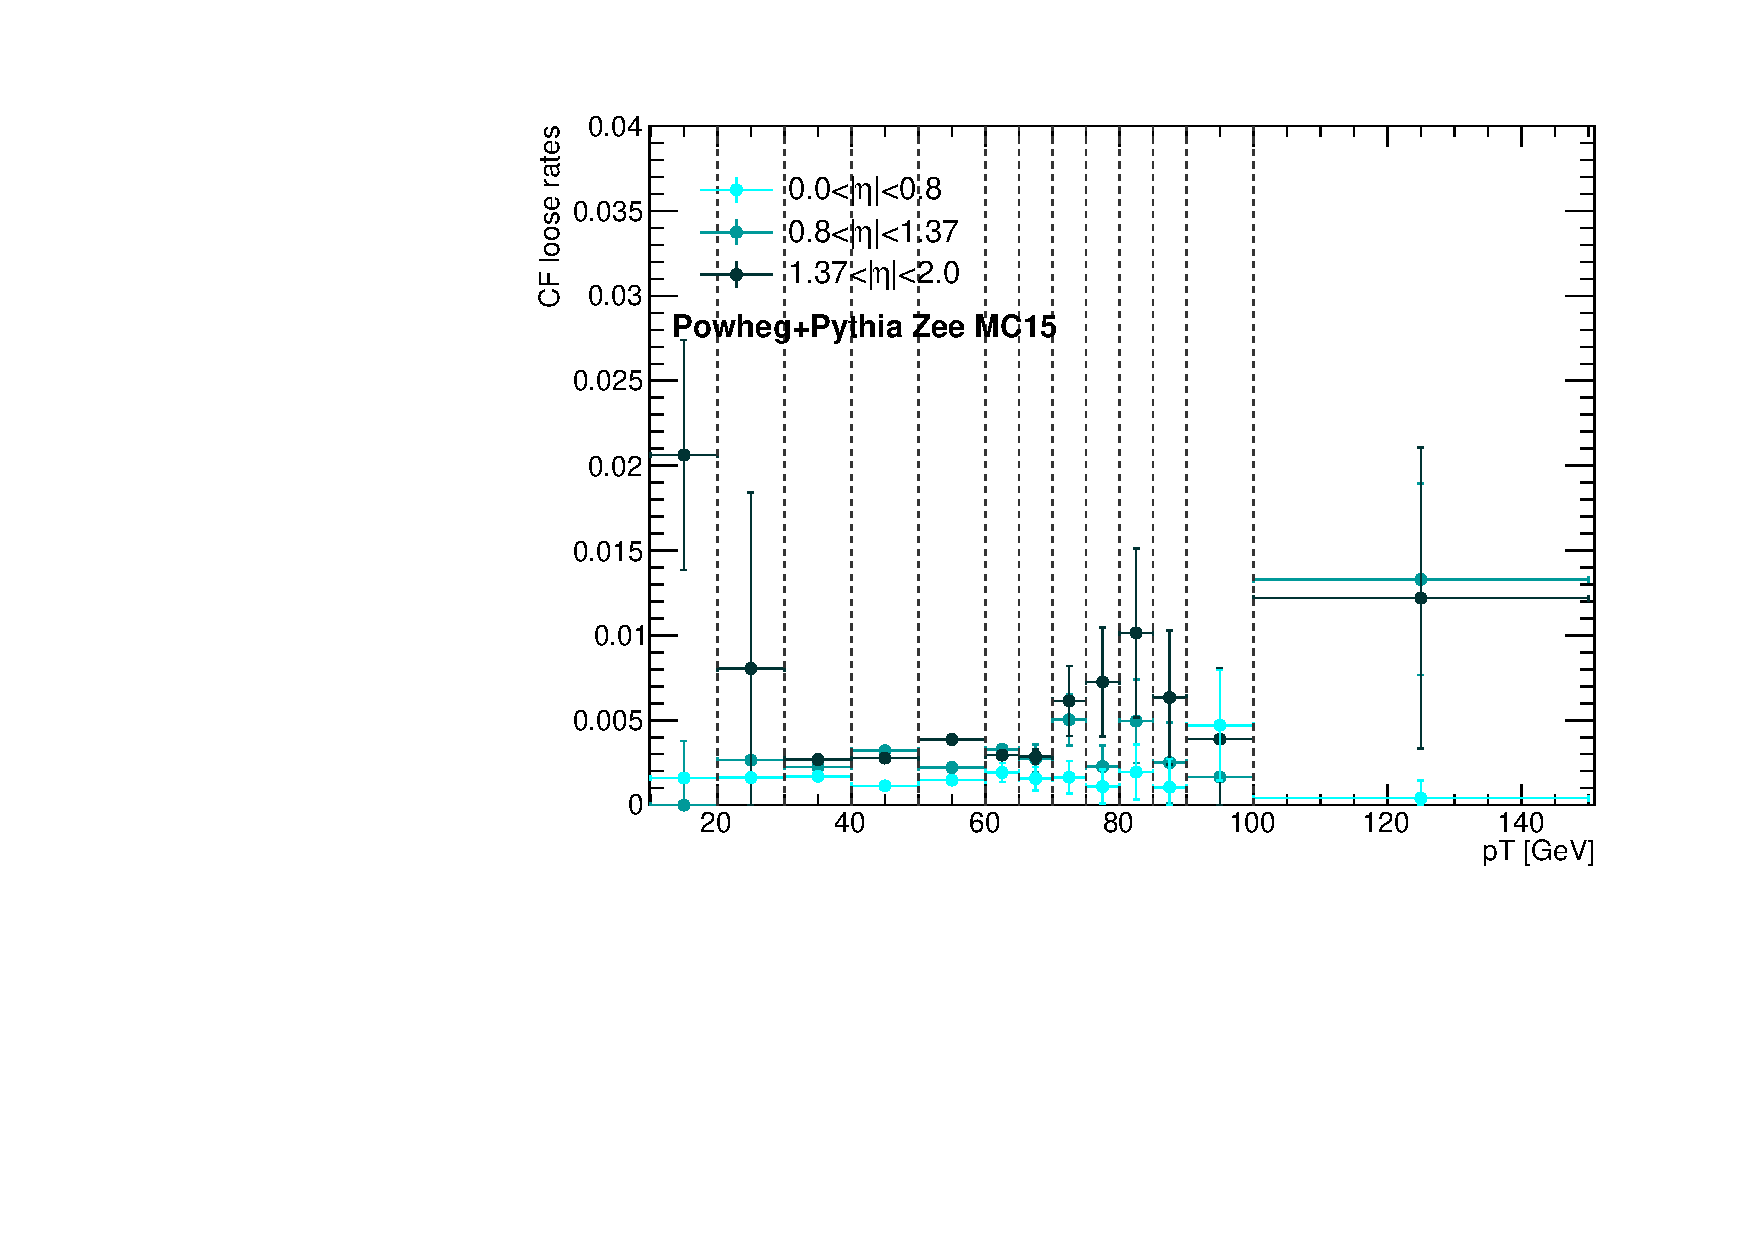
\includegraphics[width=\textwidth]{CFratesLOOSEVSpt_MC15}
	\caption{MC, baseline-failing-signal}\label{fig:Chflip_looseMC}
\end{subfigure}
\caption{Charge-flip rate as measured in data (left) and MC (right). 
Only the statistical uncertainty is displayed. The last \pt bin is inclusive.}
\label{fig:ChFlip_Rate}
\end{figure}

The charge-flip rates measured in data and MC are shown on Figure~\ref{fig:ChFlip_Rate}. 
 In data, the nominal rates (Figure~\ref{fig:Chflip_nominalData}) go up to $\sim$0.1\% in the barrel region ($|\eta| < 1.37$), 
 while it increases up to $\sim$0.2\% in the end-cap region ($|\eta > 1.37|$). 
 For baseline electrons failing signal requirements (Figure~\ref{fig:Chflip_looseData}), 
 the rates are in general greater than the nominal ones in every bin, as expected. The charge-flip rates for these electrons go up to $\sim$0.5\% in the barrel region and up 1\% in the end-cap region. Compared to the rates used in the previous version of the analysis~\cite{ATLAS-CONF-2016-037}, the central values are much lower now. After suppressing the charge flip events with the charge-flip 
electron BDT classifier described in Section~\ref{subsec:strategy.sel.obj}, 
the charge flip rates are strongly reduced for both signal and baseline-failing-signal electrons (up to a factor 20 in some bins). Figure~\ref{fig:ETA_SS_BDTEL}
illustrates the charge flip background reduction in a loose selection.
\begin{figure}[htb!]
\centering
\begin{subfigure}[t]{0.66\textwidth}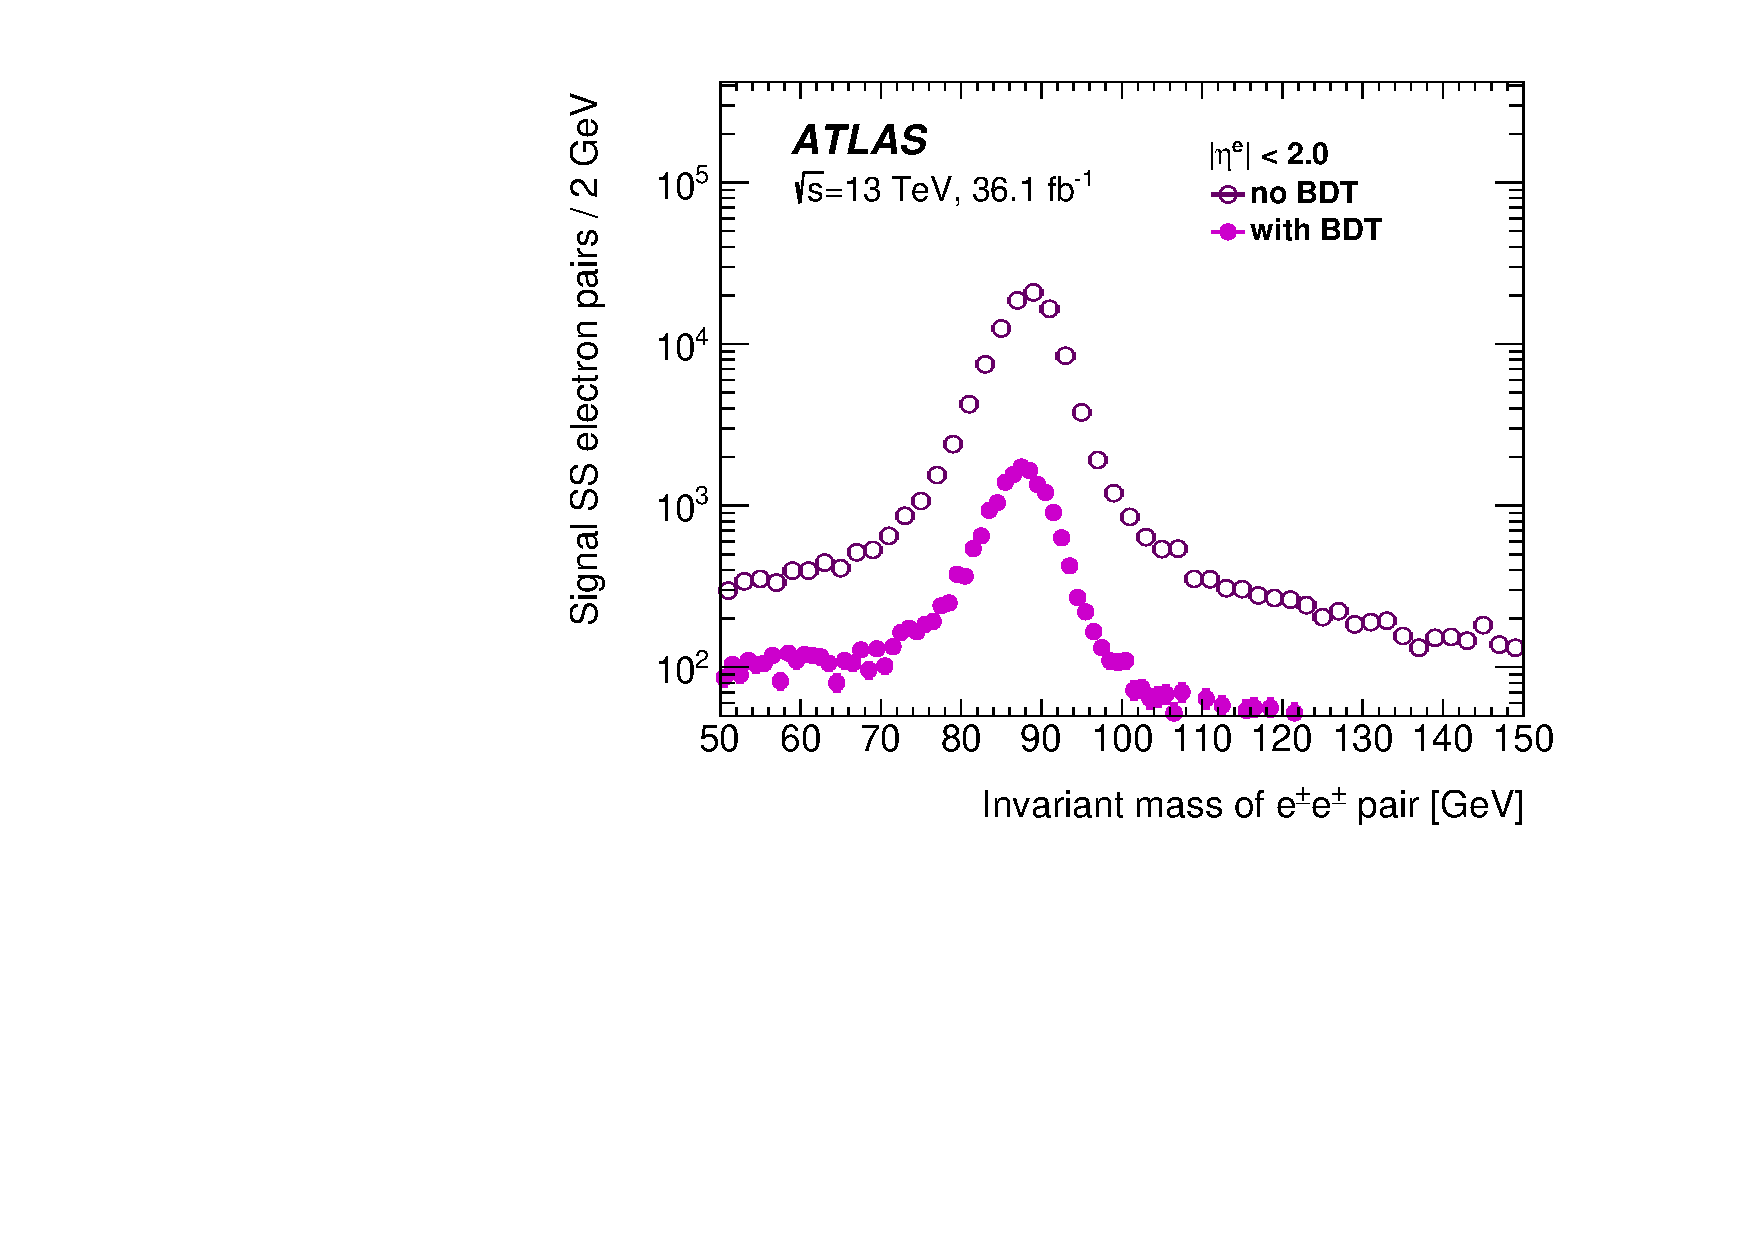
\includegraphics[width=\textwidth]{ETA_SS_BDTEL}\end{subfigure}
\caption{Invariant mass of the signal $e^{\pm} e^{\pm}$ pair distribution with (full markers) and without (open markers) charge-flip electron BDT selection applied.
}
\label{fig:ETA_SS_BDTEL}
\end{figure}
Below 30~\GeV\, the statistics are very low for the loose measurement; however, these results are used only to measure the electron fake rate and, as illustrated in Figure~\ref{Figurefakes_preselection_electron}, in this \pt interval the charge flip background is negligible.
% while the statistical uncertainties decreased significantly given the increase of up to a factor three in data luminosity. 

The charge-flip rates in MC (Figure.~\ref{fig:Chflip_nominalMC},~\ref{fig:Chflip_looseMC}) 
are obtained by applying the same methodology as in data. 
Generally, the rates are not very far from data, validating the use of MC to predict charge-flip background 
in several of the optimization studies presented in this document. 
In addition, a closure test is performed on $t\bar t$ MC, 
checking that weighted OS events can reproduce the distribution of SS charge-flip events (identified by truth-matching). 
A good overall agreement is found, largely within the assigned uncertainties
as shown in Figure~\ref{fig:ChargeFlip_ClosureTest}. 

\begin{figure}[htb!]
\centering
{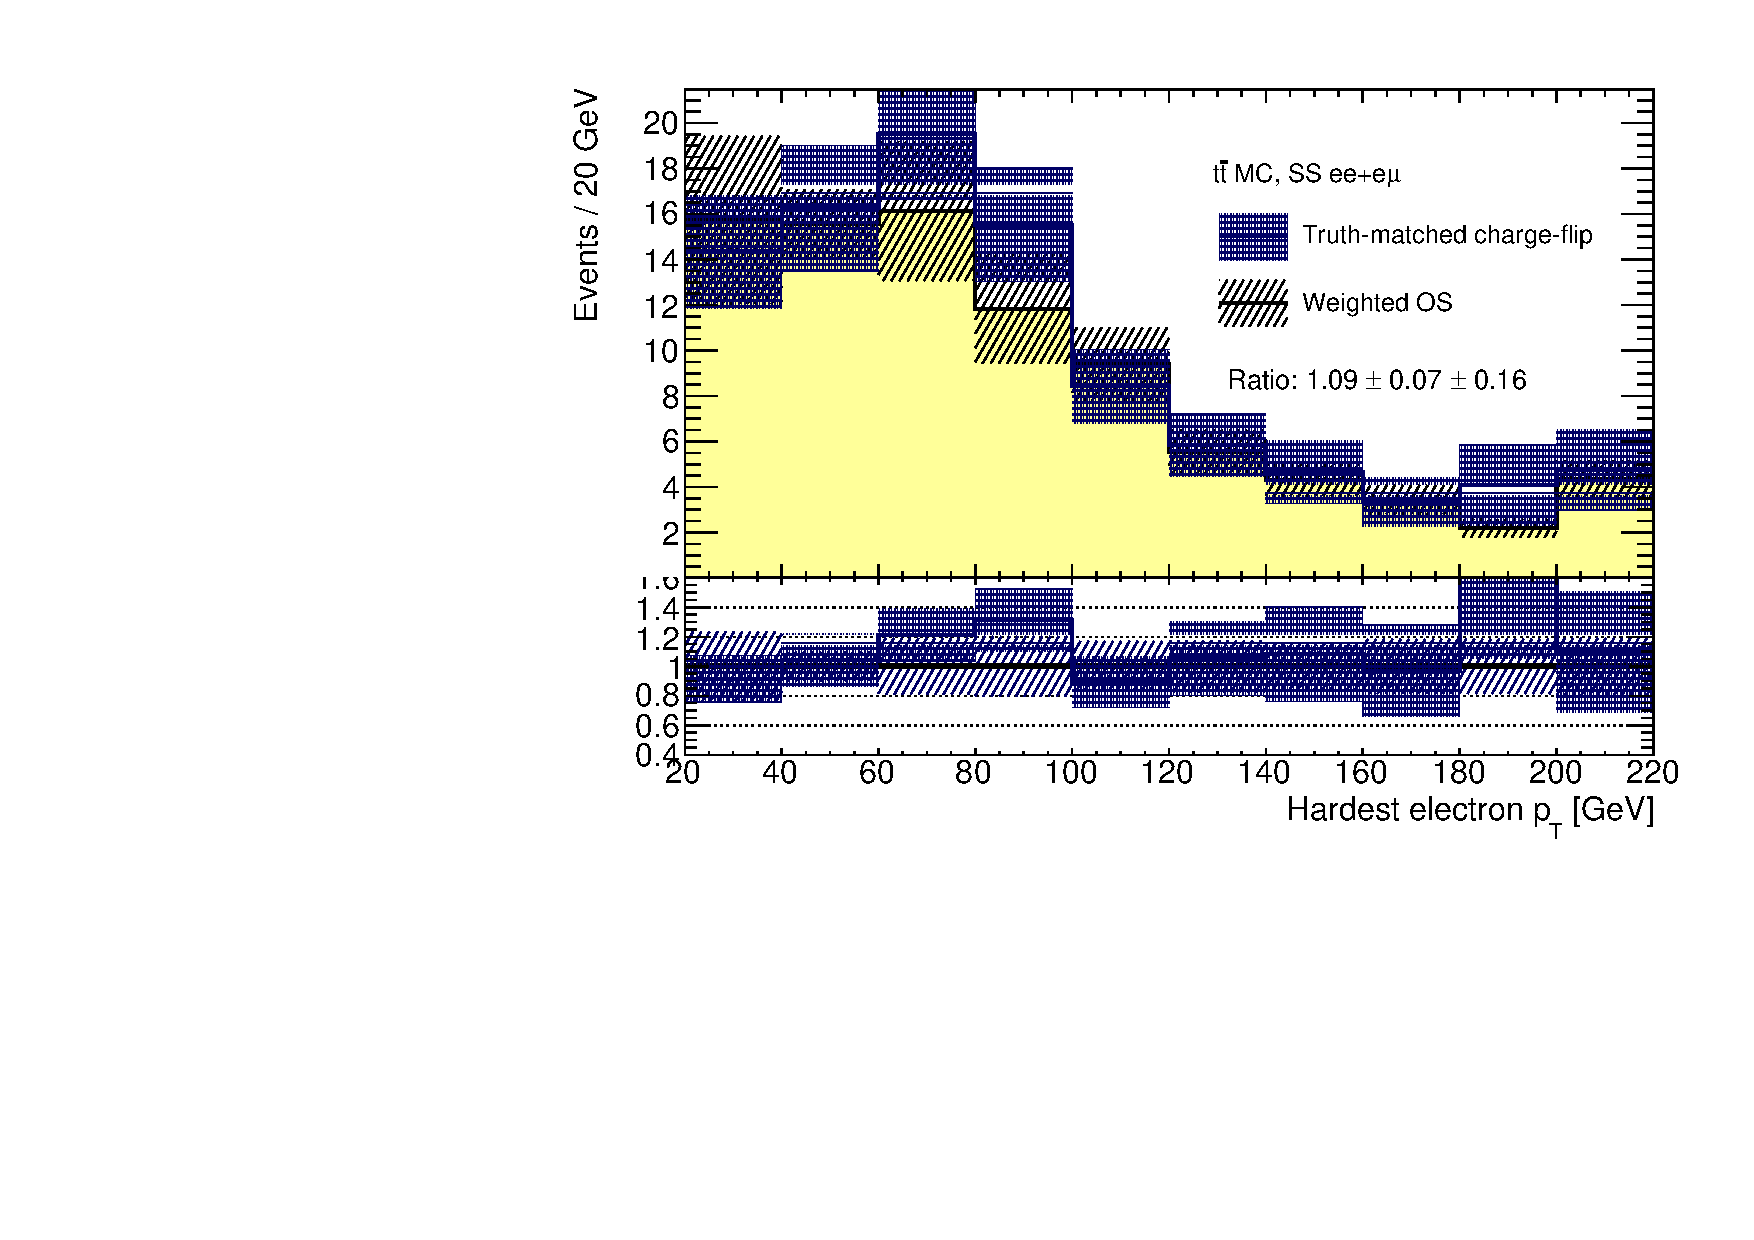
\includegraphics[width=0.49\textwidth]{Closure_HardestElectronPt}}
{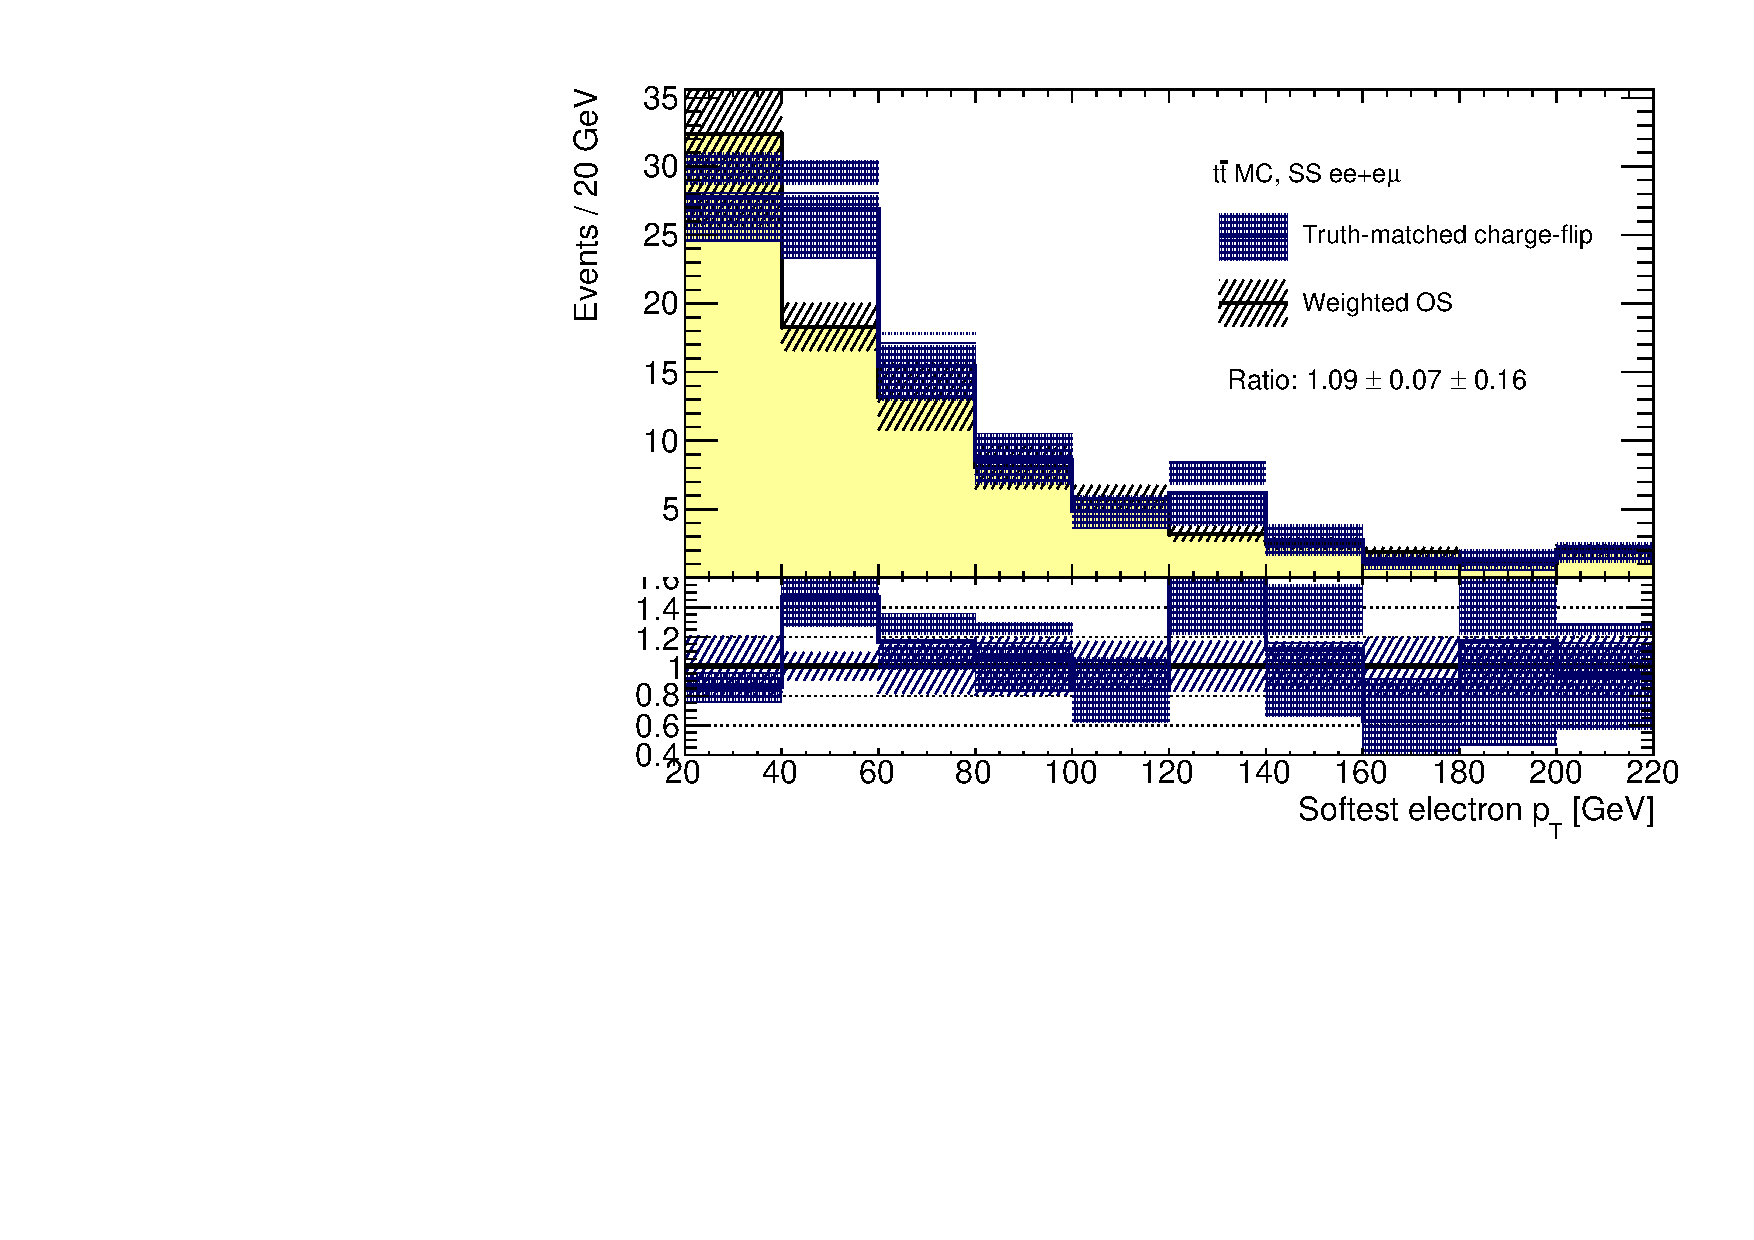
\includegraphics[width=0.49\textwidth]{Closure_SoftestElectronPt}}
{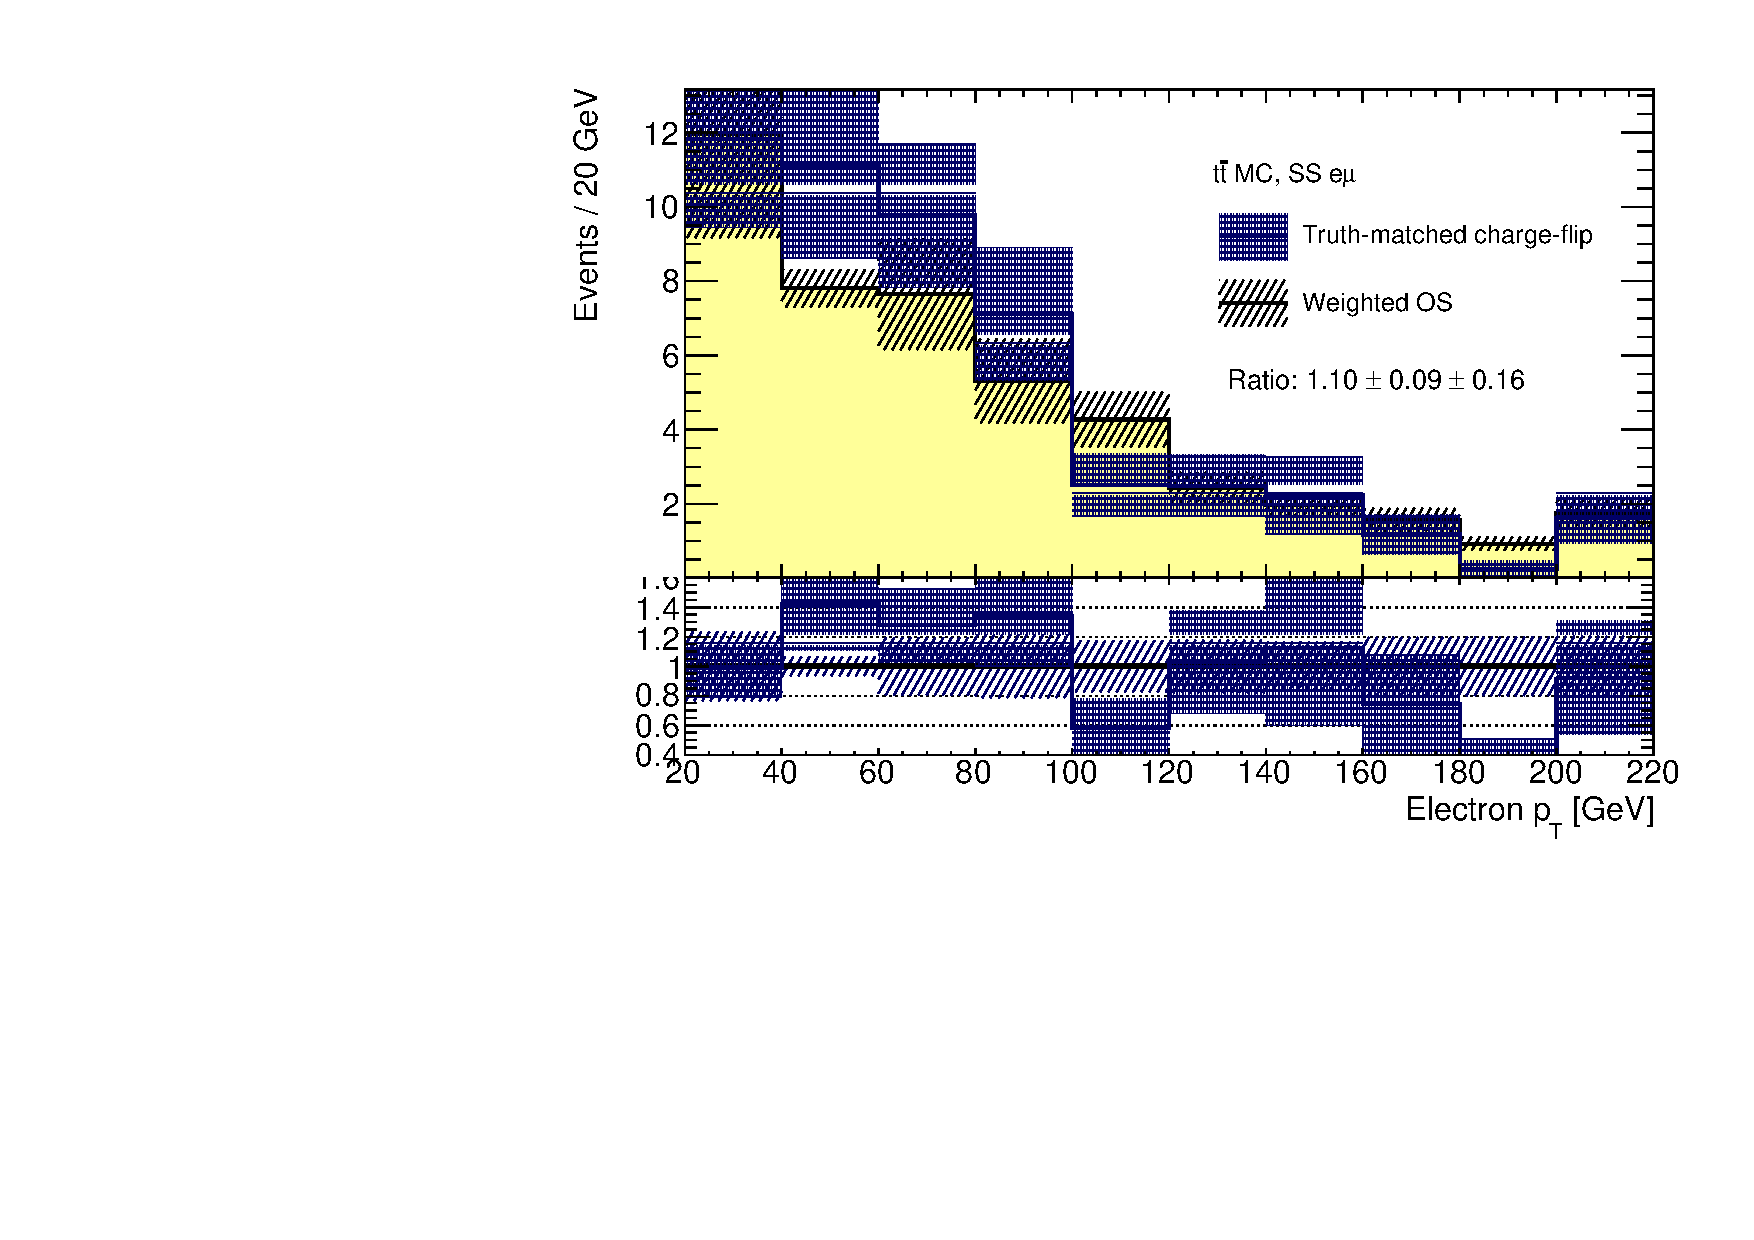
\includegraphics[width=0.49\textwidth]{Closure_EMU_ElectronPt}}
%{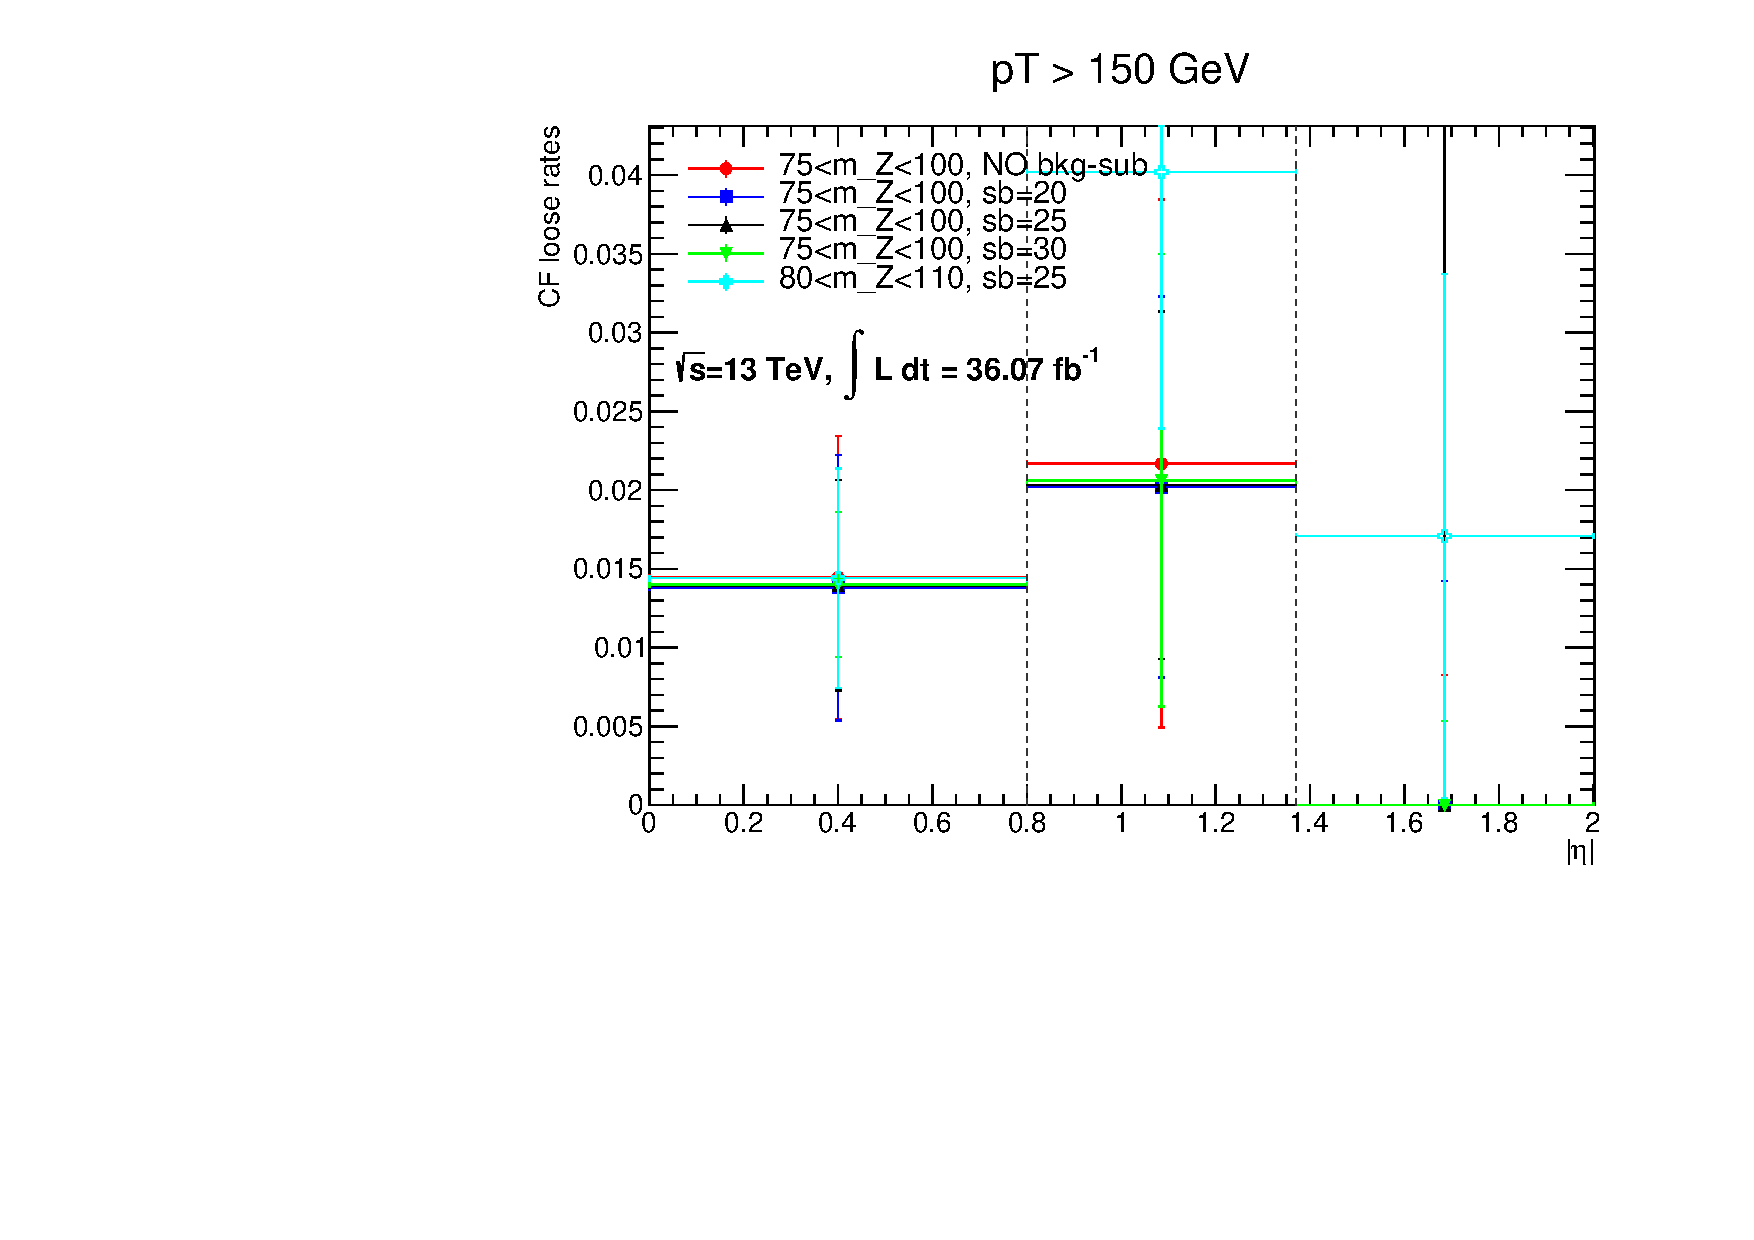
\includegraphics[width=0.49\textwidth]{CFratesLOOSE___SYStypes___PTbin13}}
\caption{Closure test for the charge-flip background prediction, for simulated $t\bar t$ events 
using charge-flip rates measured in $Z\to ee$ MC 
(with the systematic uncertainties from the data measurements, though). 
Events are selected in the $e\mu$ and $ee$ channels, using signal leptons only, 
and charge-flipped electrons are identified by truth-matching. 
}
\label{fig:ChargeFlip_ClosureTest}
\end{figure}

\subsection*{Systematic uncertainties}
\label{subsec:chargeflip_uncertainties}

%% \begin{figure}[t!]
%% \centering
%% \begin{tabular}{rr}
%% \begin{subfigure}[b]{0.5\textwidth}
%% 	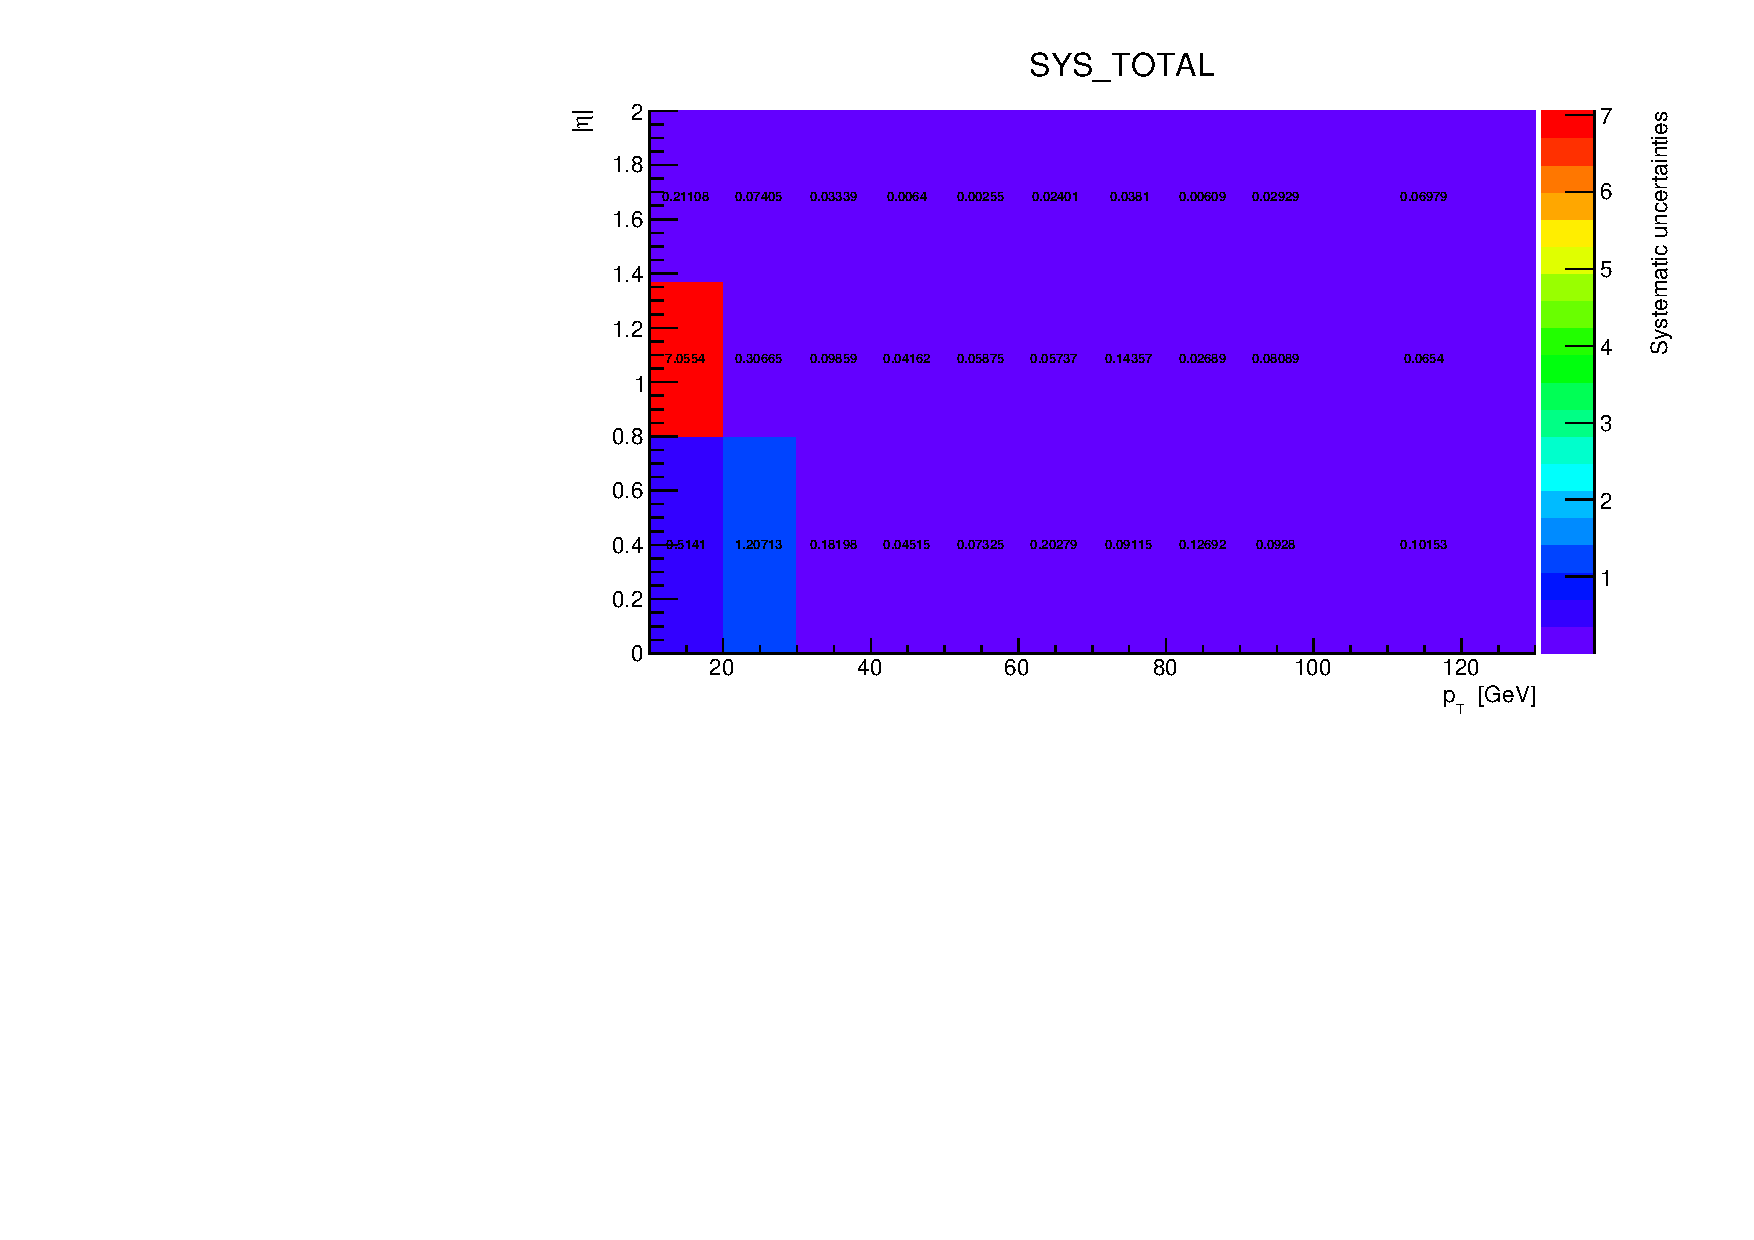
\includegraphics[width=\textwidth]{2D_histo_SYS_TOTAL}\caption{}\label{fig:bkg.chargeflip.2D_histo_SYS_TOTAL}
%% \end{subfigure} &
%% \begin{subfigure}[b]{0.5\textwidth}
%% 	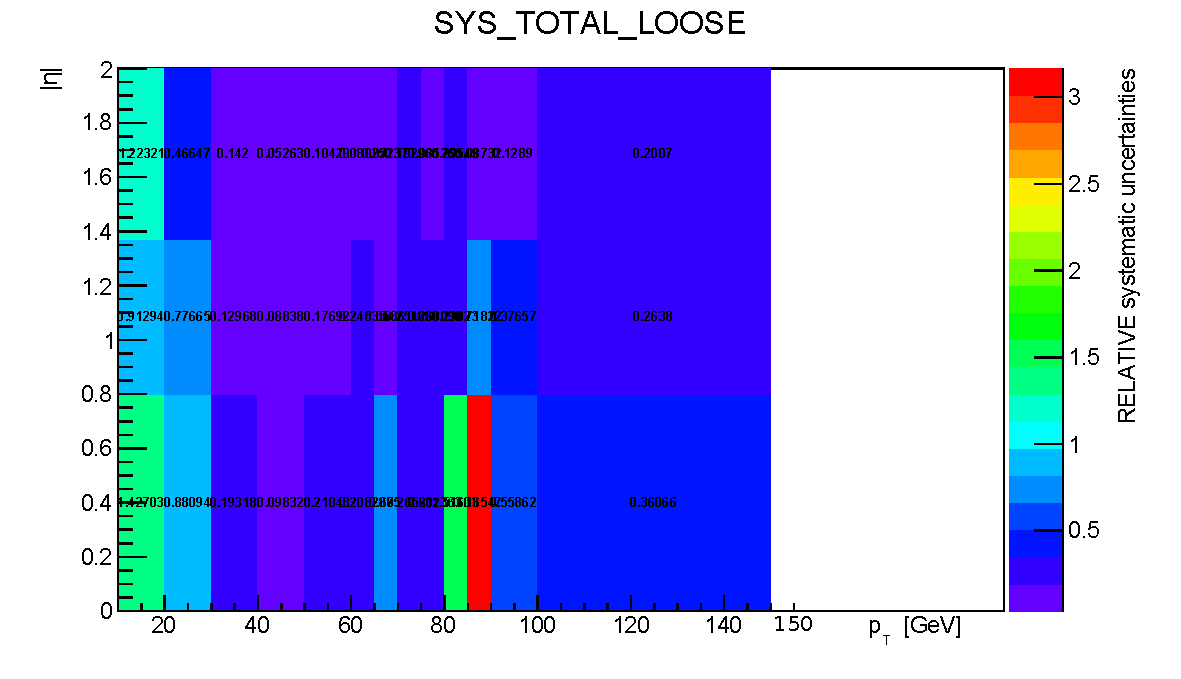
\includegraphics[width=\textwidth]{2D_histo_SYS_TOTAL_LOOSE}\caption{}\label{fig:bkg.chargeflip.2D_histo_SYS_TOTAL_LOOSE}
%% \end{subfigure}
%% \end{tabular}
%% \caption{Total systematic uncertainties on the charge-flip rates for electrons satisfying the signal requirements (\ref{fig:bkg.chargeflip.2D_histo_SYS_TOTAL}),
%% and for baseline electrons failing the signal requirements (\ref{fig:bkg.chargeflip.2D_histo_SYS_TOTAL_LOOSE}). 
%% }
%% \label{fig:ChFlip_SYS_Total}
%% \end{figure}

The main uncertainties on the measured charge-flip rates come from the presence of background and the way it is estimated. To assess them, variations of the selection and background estimation are considered: 
\begin{itemize}
\item[1)] $75<m_{ee}<100~\GeV$, no background subtraction;
\item[2)] $75<m_{ee}<100~\GeV$, sidebands of 20~\GeV;
\item[3)] $75<m_{ee}<100~\GeV$, sidebands of 25~\GeV~(nominal measurement);
\item[4)] $75<m_{ee}<100~\GeV$, sidebands of 30~\GeV;
\item[5)] $80<m_{ee}<100~\GeV$, sidebands of 20~\GeV.
\end{itemize}

The effect of applying the background subtraction itself is evaluated by comparing configurations 1 and 3. 
The impact of the width of the $m_{ee}$ chosen for the measurement is  by comparing configurations 3 and 5, 
while the sideband width effects are evaluated by comparing configuration 3 and 2, or 3 and 4. 
The largest deviation in each bin is taken as the systematic uncertainty on the charge-flip rate.

%The resulting systematic uncertainties on the charge-flip rates are presented in Figure~\ref{fig:ChFlip_SYS_Total}. 

For the signal electrons charge-flip rates the systematic uncertainties vary in general between 2\% and 20\% (increasing up to $>50\%$ in the region with $\pt < 10~\GeV$), whereas for baseline-failing-signal electrons they vary between 3\% and 30\% (increasing up to $>50\%$ in the region with $\pt < 10~\GeV$). Part of these large values, at low \pt and in the [80,90]~\GeV~\pt interval, can be explained by large statistical fluctuations between the different configurations.


\subsection{Expected yields in signal regions}
\label{subsec:fakes_yields}

The expected yield for processes with fake leptons, 
estimated with the method described in sections~\ref{subsec:fakes_matrix} and~\ref{subsec:fakes_mctemplate}, 
are presented in Table~\ref{tab:fakes_sr_yields} for the signal regions. 
They are compared for cross-check with the alternative ABCD prediction (section~\ref{subsec:fakes_abcd}), 
and are all found to be consistent with each other. 

The final numbers retained for the fake lepton background estimate (also shown in the tables) 
are taken as the weighted-average of the predictions from the matrix method and the MC template; 
the weights are based on the statistical component, and the systematic uncertainties are propagated 
assuming conservatively a full correlation between the two methods (although they are in fact largely independent!). 
The central value and statistical/systematic uncertainties are therefore: 

\begin{align}
&\left(w\zeta_1 + (1-w)\zeta_2\right) 
\pm \sqrt{w^2\left(\Delta\zeta_1^\text{(stat)}\right)^2 + (1-w)^2\left(\Delta\zeta_2^\text{(stat)}\right)^2} 
\pm \left(w\Delta\zeta_1^\text{(syst)} + (1-w)\Delta\zeta_2^\text{(syst)}\right)\\
&\qquad\text{ with }w=\frac{\left(\Delta\zeta_2^\text{(stat)}\right)^2}{\left(\Delta\zeta_1^\text{(stat)}\right)^2+\left(\Delta\zeta_2^\text{(stat)}\right)^2}\notag
\end{align}

When the estimated value is too small(below 0.15), the expected yield is set to $0.15\pm 0.15$, 
to cover for possibilities of an under-fluctuation of the number of baseline-not-signal leptons 
when applying the matrix method, as well as lack of statistics in the MC samples for the other method. 
 
This upper bound is inflated if the original combined prediction $x\pm\Delta x$ 
is such that its plus-one-sigma variation exceeds the upper bound, that is $\delta=(x+\Delta x)>0.30$; 
in that case the final retained number is $(\delta/2)\pm (\delta/2)$. 
There is no such instance in the current SR estimates, though, as can be seen in the table.  

\begin{table}[!htb]
\caption{Expected yields for background processes with fake leptons,
in the signal regions proposed in Section~\ref{sec:signalregions}, shown for 36 \ifb. 
Uncertainties include all statistical and systematic sources for the nominal estimate (except ABCD, cf section~\ref{subsec:fakes_abcd}). 
}
\label{tab:fakes_sr_yields}
\centering
\resizebox{\textwidth}{!}{
\begin{tabular}{|c||c|c|c||c|}\hline
      Region &              Matrix method   &   Template method   &       ABCD method   &     Retained estimate  \\\hline
% v52, updated uncertainties and real efficiencies
    Rpc2L0bH & $ 0.83 \pm  0.56 \pm  0.74$  &  $1.00 \pm 0.96 \pm 0.81$  &  $0.36\pm 0.25 \pm 0.06$   &  $ 0.87 \pm  0.48 \pm  0.76$  \\
    Rpc2L0bS & $ 1.51 \pm  0.60 \pm  0.66$  &  $1.68 \pm 1.02 \pm 1.26$  &  $0.66\pm 0.39\pm 0.22$    &  $ 1.55 \pm  0.52 \pm  0.81$  \\
    Rpc2L1bH & $ 3.54 \pm  1.62 \pm  3.12$  &  $2.07 \pm 0.63 \pm 1.56$  &  $2.06\pm 0.32\pm 0.16$    &  $ 2.26 \pm  0.59 \pm  1.76$  \\
    Rpc2L1bS & $ 2.65 \pm  1.21 \pm  1.89$  &  $02.33 \pm 01.17 \pm 02.10$  &   $2.7\pm 0.6\pm 1.5$     &  $ 2.48 \pm  0.84 \pm  2.00$  \\ 
    Rpc2L2bH & $-0.11 \pm  0.11 \pm  0.18$  &  $<0.5$  &  $0.10\pm 0.05\pm 0.03$    &  $ 0.15 \pm  0.15 \pm  0.00$  \\
    Rpc2L2bS & $ 1.31 \pm  1.07 \pm  1.65$  &  $0.41 \pm 0.33 \pm 0.45$  &  $1.1\pm 0.2\pm 0.4$       &  $ 0.49 \pm  0.32 \pm  0.55$  \\
    Rpc2Lsoft1b & $ 4.75 \pm  1.42 \pm  2.64$  &  $2.48 \pm 1.32 \pm 1.86$  &  $1.2\pm 0.3\pm 1.2$       &  $ 3.53 \pm  0.97 \pm  2.22$  \\
    Rpc2Lsoft2b & $ 1.91 \pm  1.18 \pm  1.63$  &  $1.66 \pm 0.66 \pm 1.28$  &  $0.72\pm 0.19\pm 0.26$    &  $ 1.72 \pm  0.58 \pm  1.36$  \\
    Rpc3L0bH & $-0.01 \pm  0.11 \pm  0.10$  &  $<0.5$  &  $<0$                      &  $ 0.15 \pm  0.15 \pm  0.00$  \\
    Rpc3L0bS & $ 2.31 \pm  1.50 \pm  2.63$  &  $0.21 \pm 0.15 \pm 0.16$  &  $<0$                      &  $ 0.23 \pm  0.15 \pm  0.18$  \\
    Rpc3L1bH & $ 0.57 \pm  0.43 \pm  0.50$  &  $0.42 \pm 0.29 \pm 0.32$  &  $<0$                      &  $ 0.47 \pm  0.24 \pm  0.38$  \\
    Rpc3L1bS & $ 4.94 \pm  1.83 \pm  2.96$  &  $3.55 \pm 1.80 \pm 2.76$  &  $1.0\pm 0.9\pm 0.1$       &  $ 4.23 \pm  1.28 \pm  2.86$  \\
    Rpc3LSS1b & $-0.18 \pm  1.24 \pm  2.85$  &  $0.90 \pm 0.14 \pm 0.69$  &  $-$                       &  $ 0.89 \pm  0.14 \pm  0.72$  \\
    Rpv2L0b & $ 0.14 \pm  0.22 \pm  0.27$  &  $1.02 \pm 0.96 \pm 0.76$  &  $0.13\pm 0.12\pm 0.04$    &  $ 0.18 \pm  0.21 \pm  0.29$  \\
    Rpv2L1bH & $-0.06 \pm  0.03 \pm  0.09$  &  $0.60 \pm 0.35 \pm 0.48$  &  $0.31\pm 0.11\pm 0.08$    &  $ 0.15 \pm  0.15 \pm  0.00$  \\
    Rpv2L1bM & $ 1.70 \pm  2.07 \pm  1.68$  &  $1.20 \pm 0.69 \pm 0.95$  &  $0.53\pm 0.10\pm 0.18$    &  $ 1.25 \pm  0.65 \pm  1.02$  \\
    Rpv2L1bS & $16.49 \pm  4.04 \pm 18.70$  &  $4.46 \pm 1.67 \pm 3.45$  &  $4.5\pm 0.9\pm 1.4$       &  $ 6.22 \pm  1.54 \pm  5.68$  \\
    Rpv2L2bH & $-0.04 \pm  0.02 \pm  0.04$  &  $<0.5$  &  $0.26\pm 0.08 \pm 0.07$   &  $ 0.15 \pm  0.15 \pm  0.00$  \\
    Rpv2L2bS & $ 9.67 \pm  3.29 \pm  9.04$  &  $7.24 \pm 2.36 \pm 5.43$  &  $2.7\pm 0.5\pm 1.0$       &  $ 8.07 \pm  1.92 \pm  6.66$  \\  
\hline
\hline
\end{tabular}
}
\end{table}

To check the validity and robustness of the FNP lepton estimate, 
the distributions of several discriminating variables in data are compared 
with the predicted background after various requirements on the number of jets and $b$-jets. 
Examples of such distributions are shown in Figure~\ref{fig:Bkg_distribs}, 
and illustrate that the data are described by the prediction within uncertainties. The apparent disagreement 
for \meff\ above 1 TeV in Figure~\ref{fig:VRmeff2} is covered by the large theory uncertainty for the diboson background, which is not shown 
but amounts to about 30\% for \meff\ above 1 TeV.

\begin{figure}[th!]
\centering
\begin{subfigure}[t]{0.49\textwidth}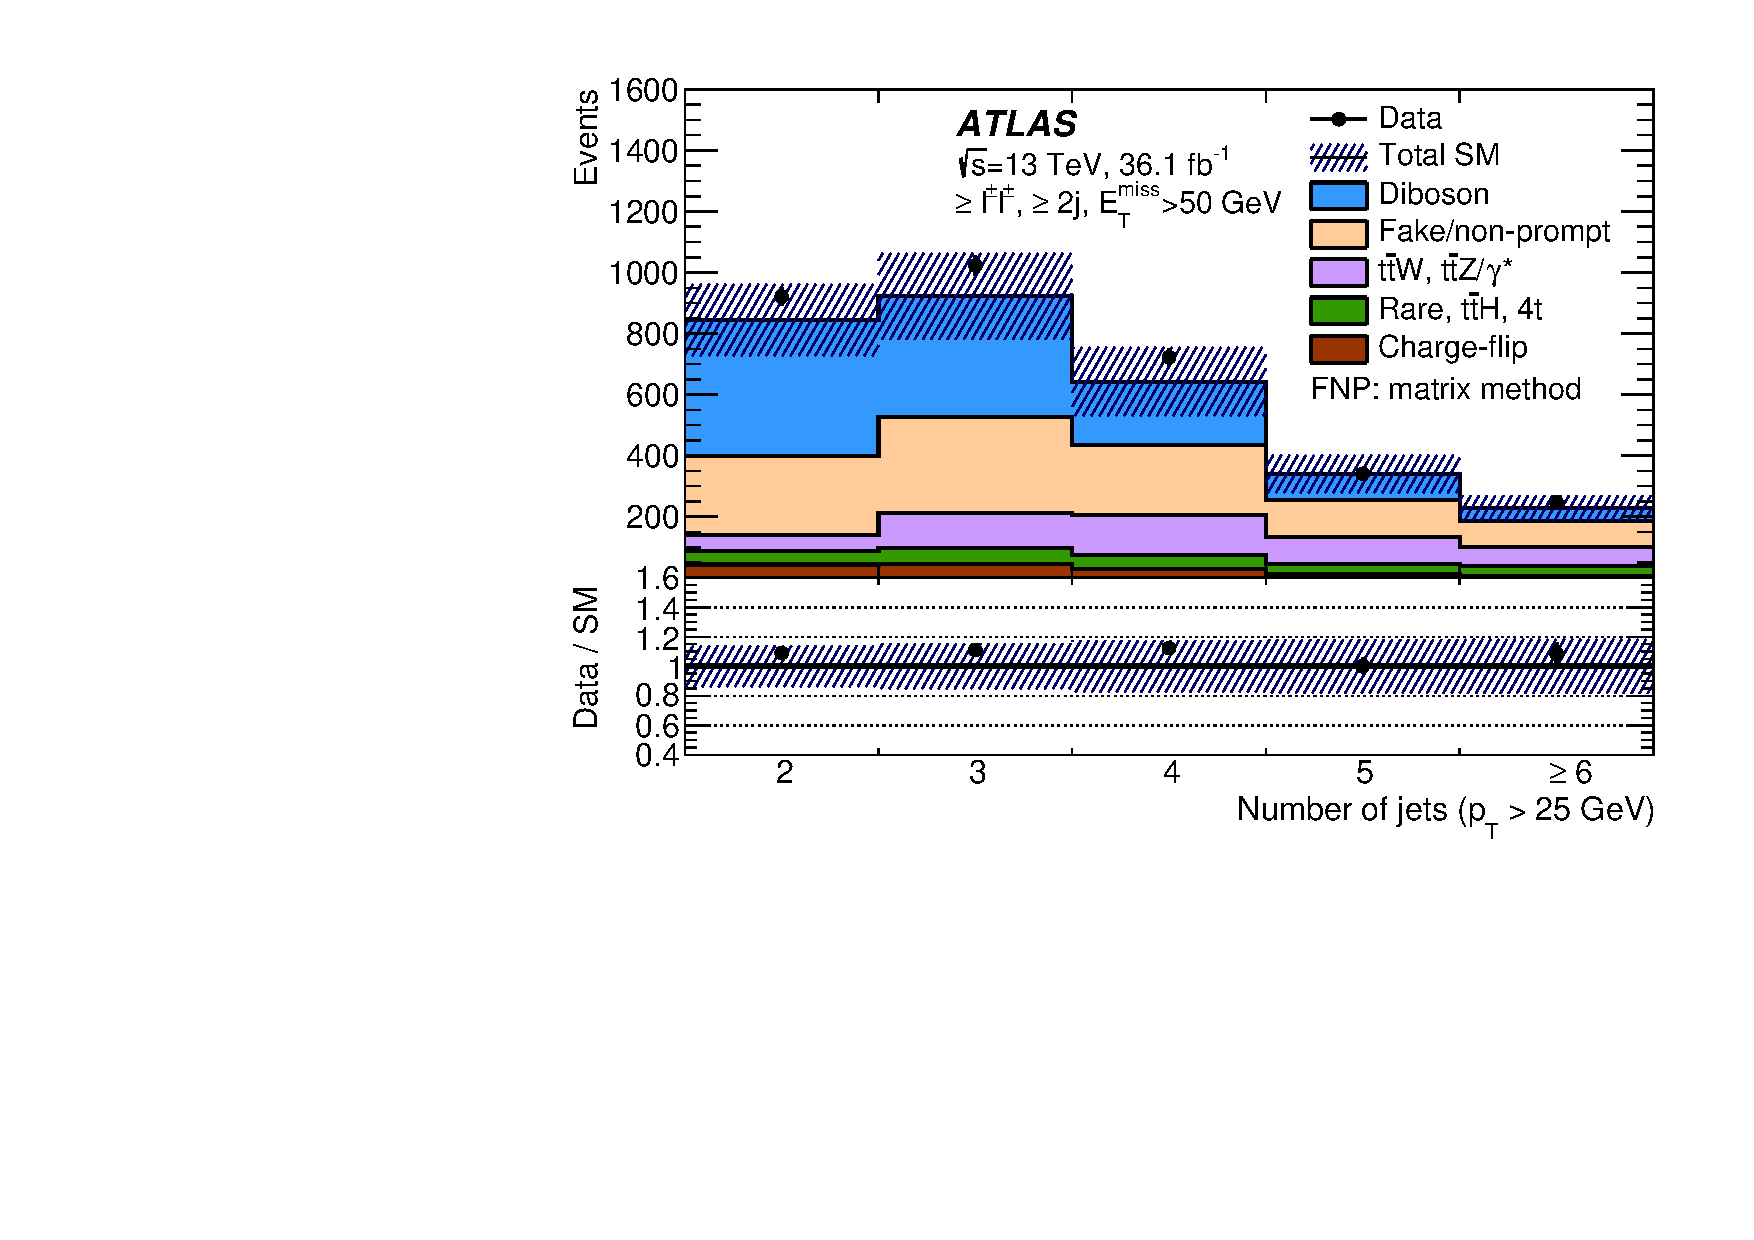
\includegraphics[width=\textwidth]{PAPER_DILEP_2JMET50_njets25}\caption{}\label{fig:VRnj}\end{subfigure}
\begin{subfigure}[t]{0.49\textwidth}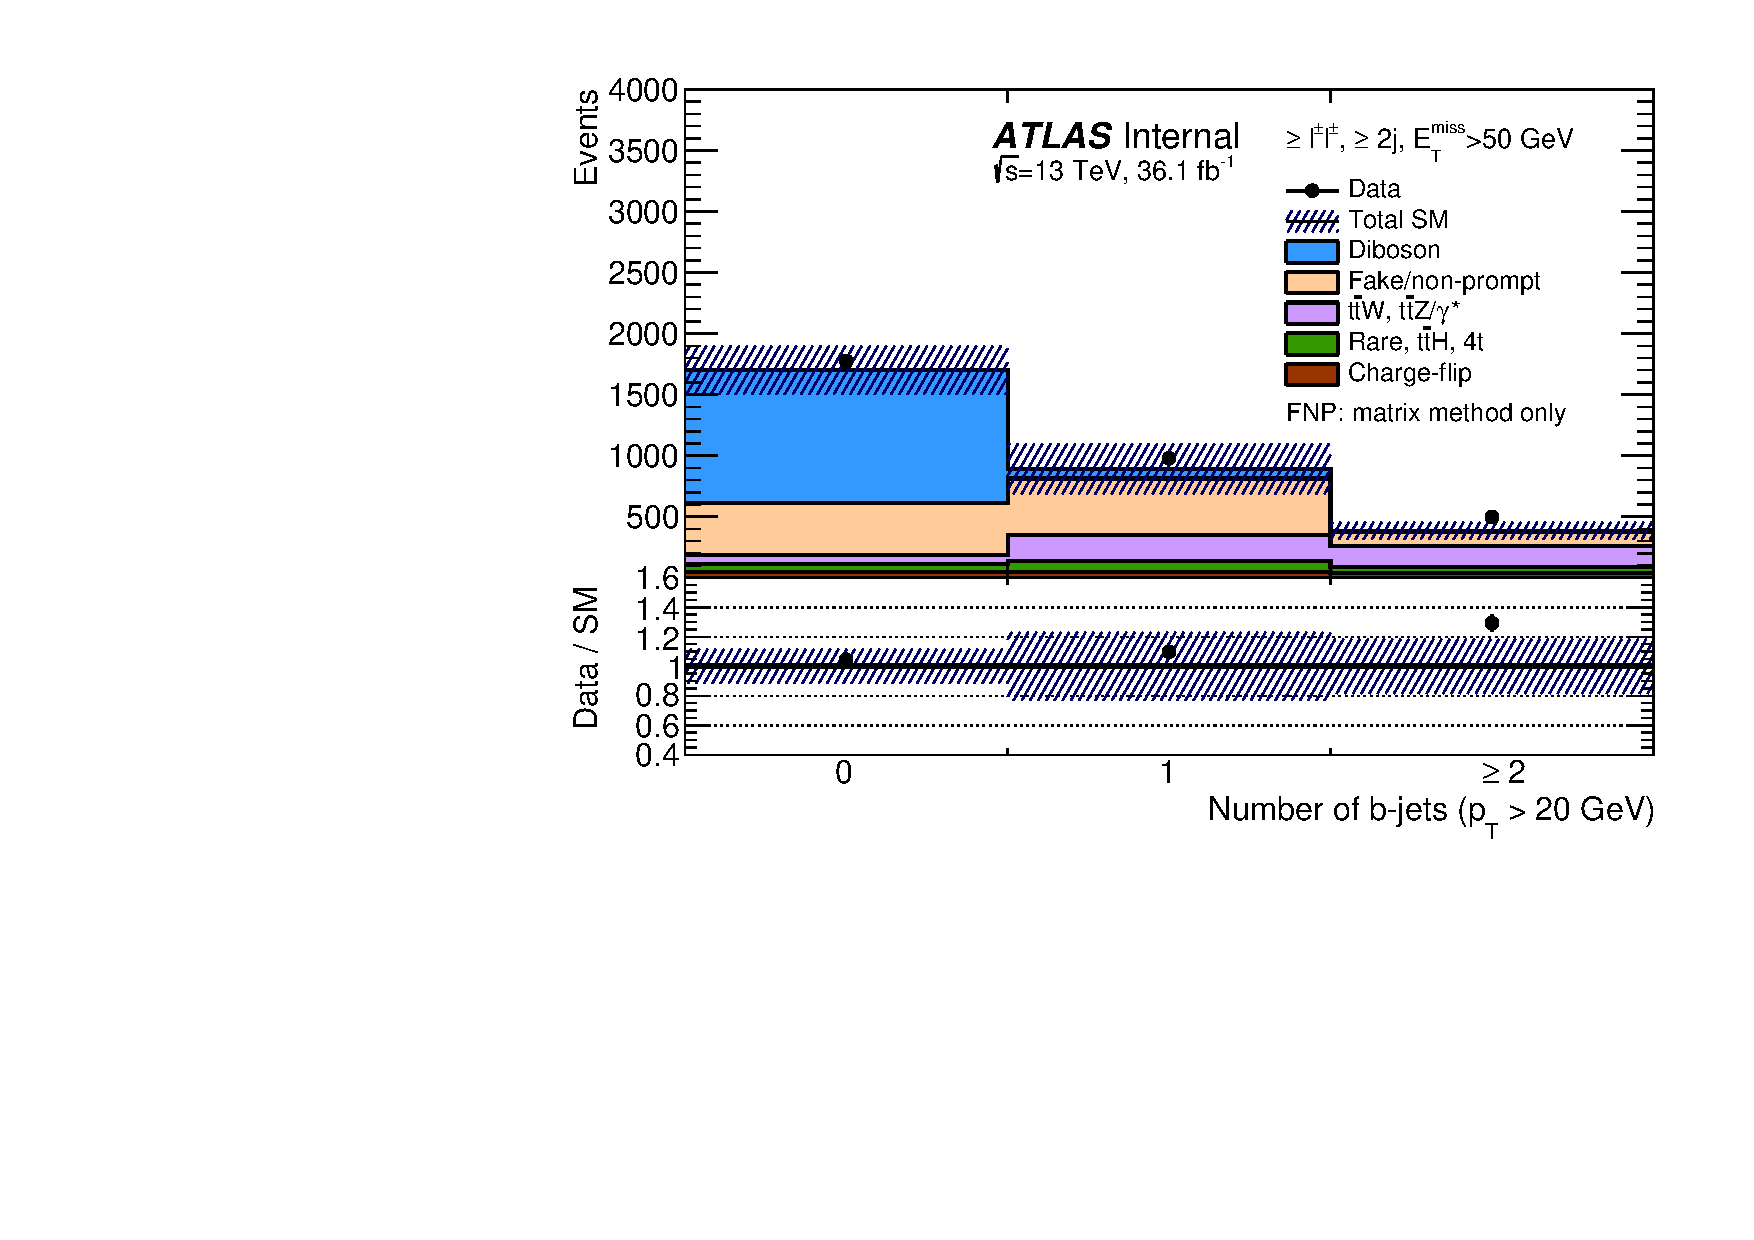
\includegraphics[width=\textwidth]{PAPER_DILEP_2JMET50_nbjets}\caption{}\label{fig:VRnb}\end{subfigure}
\begin{subfigure}[t]{0.49\textwidth}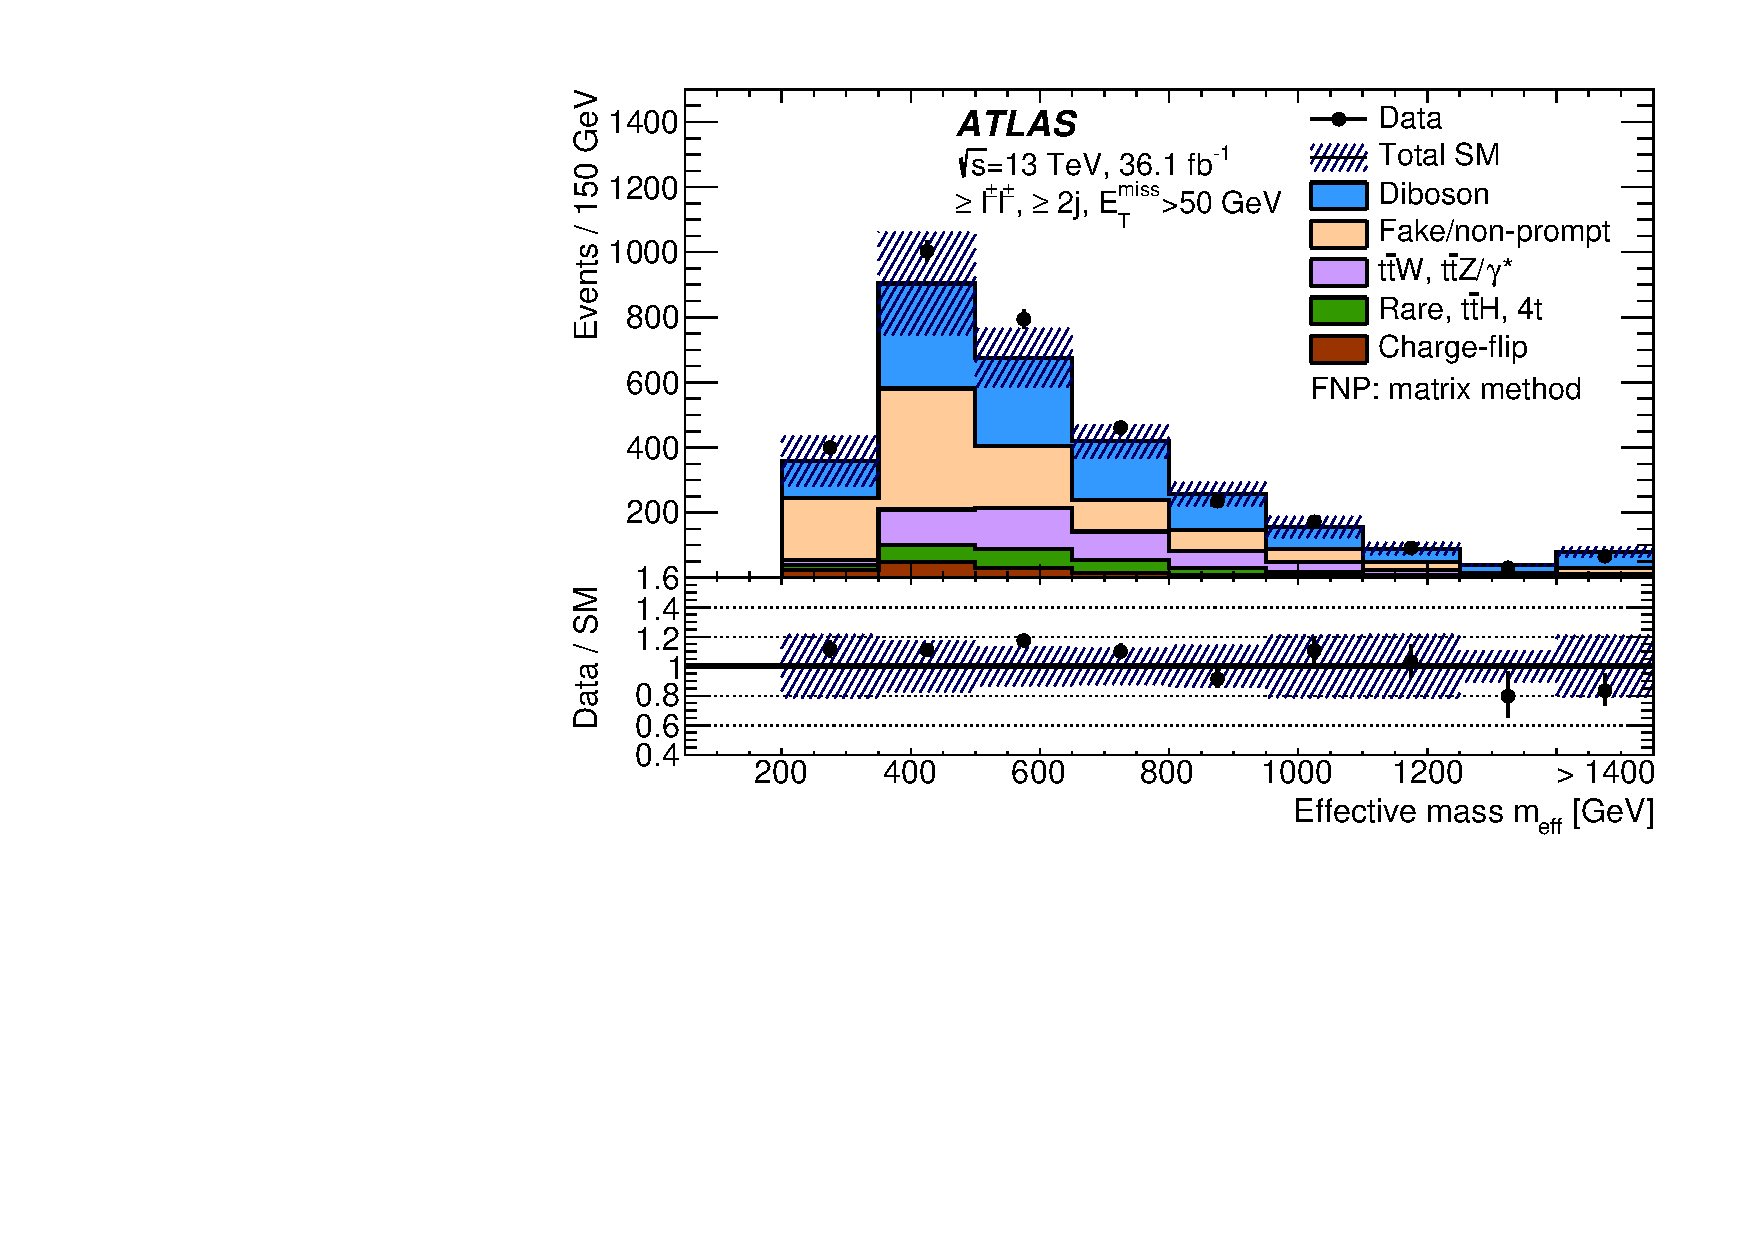
\includegraphics[width=\textwidth]{PAPER_DILEP_2JMET50_meff}\caption{}\label{fig:VRmeff1}\end{subfigure}
\begin{subfigure}[t]{0.49\textwidth}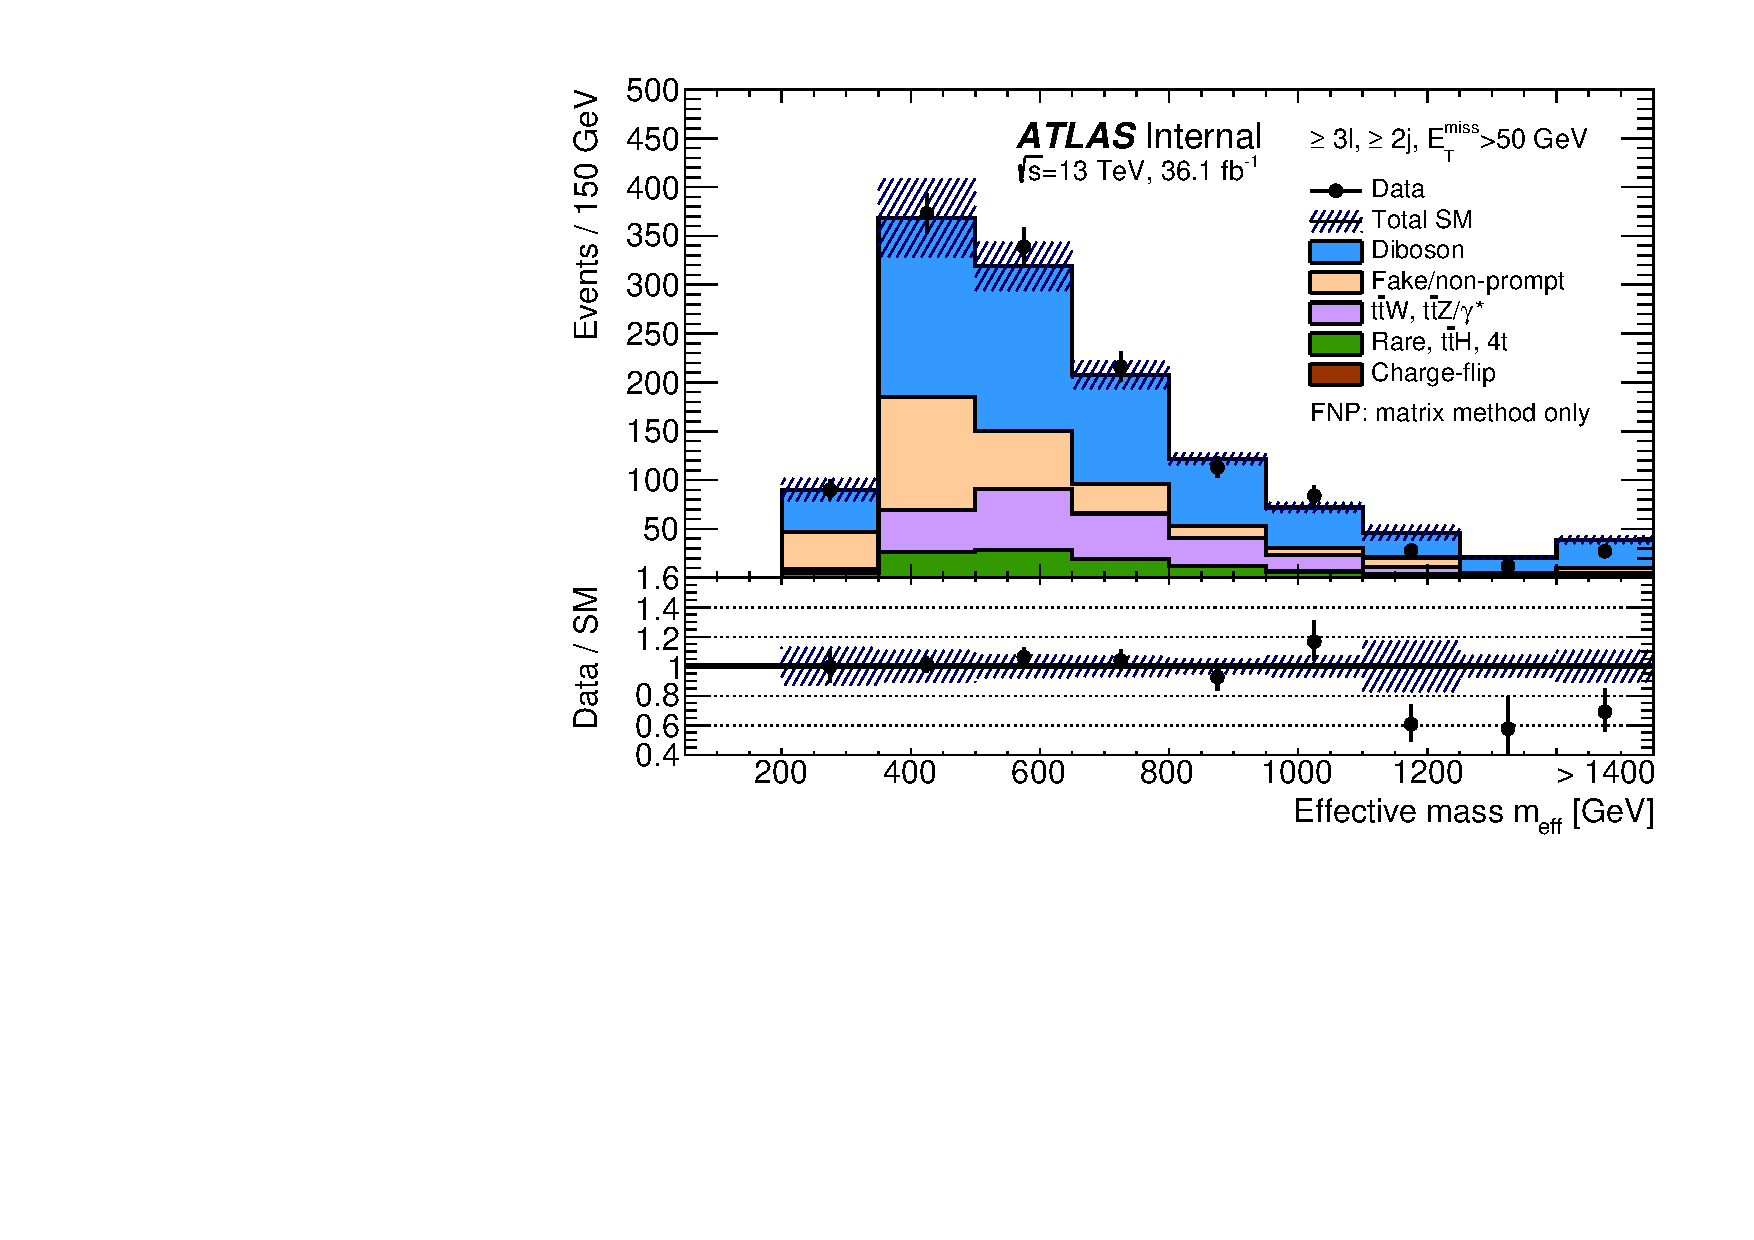
\includegraphics[width=\textwidth]{PAPER_TRILEP_2JMET50_meff}\caption{}\label{fig:VRmeff2}\end{subfigure}
\caption{
Distributions of (a) the number of jets, (b) the number of $b$-tagged jets and (c), (d) the effective mass. The distributions are made 
after requiring at least two jets ($\pT>40 \GeV$) and $\met>50 \GeV$, as well as at least two same-sign leptons ((a), (b), (c)) 
or three leptons (d). The uncertainty bands include the statistical uncertainties for the background prediction as well as the 
systematic uncertainties for fake- or non-prompt-lepton backgrounds (using the matrix method) and charge-flip electrons. Not included
are theoretical uncertainties in the irreducible background contributions.
The rare category is defined in the text.}
\label{fig:Bkg_distribs} 
\end{figure} 


\begin{figure}[htb!]
\begin{subfigure}[t]{0.49\textwidth}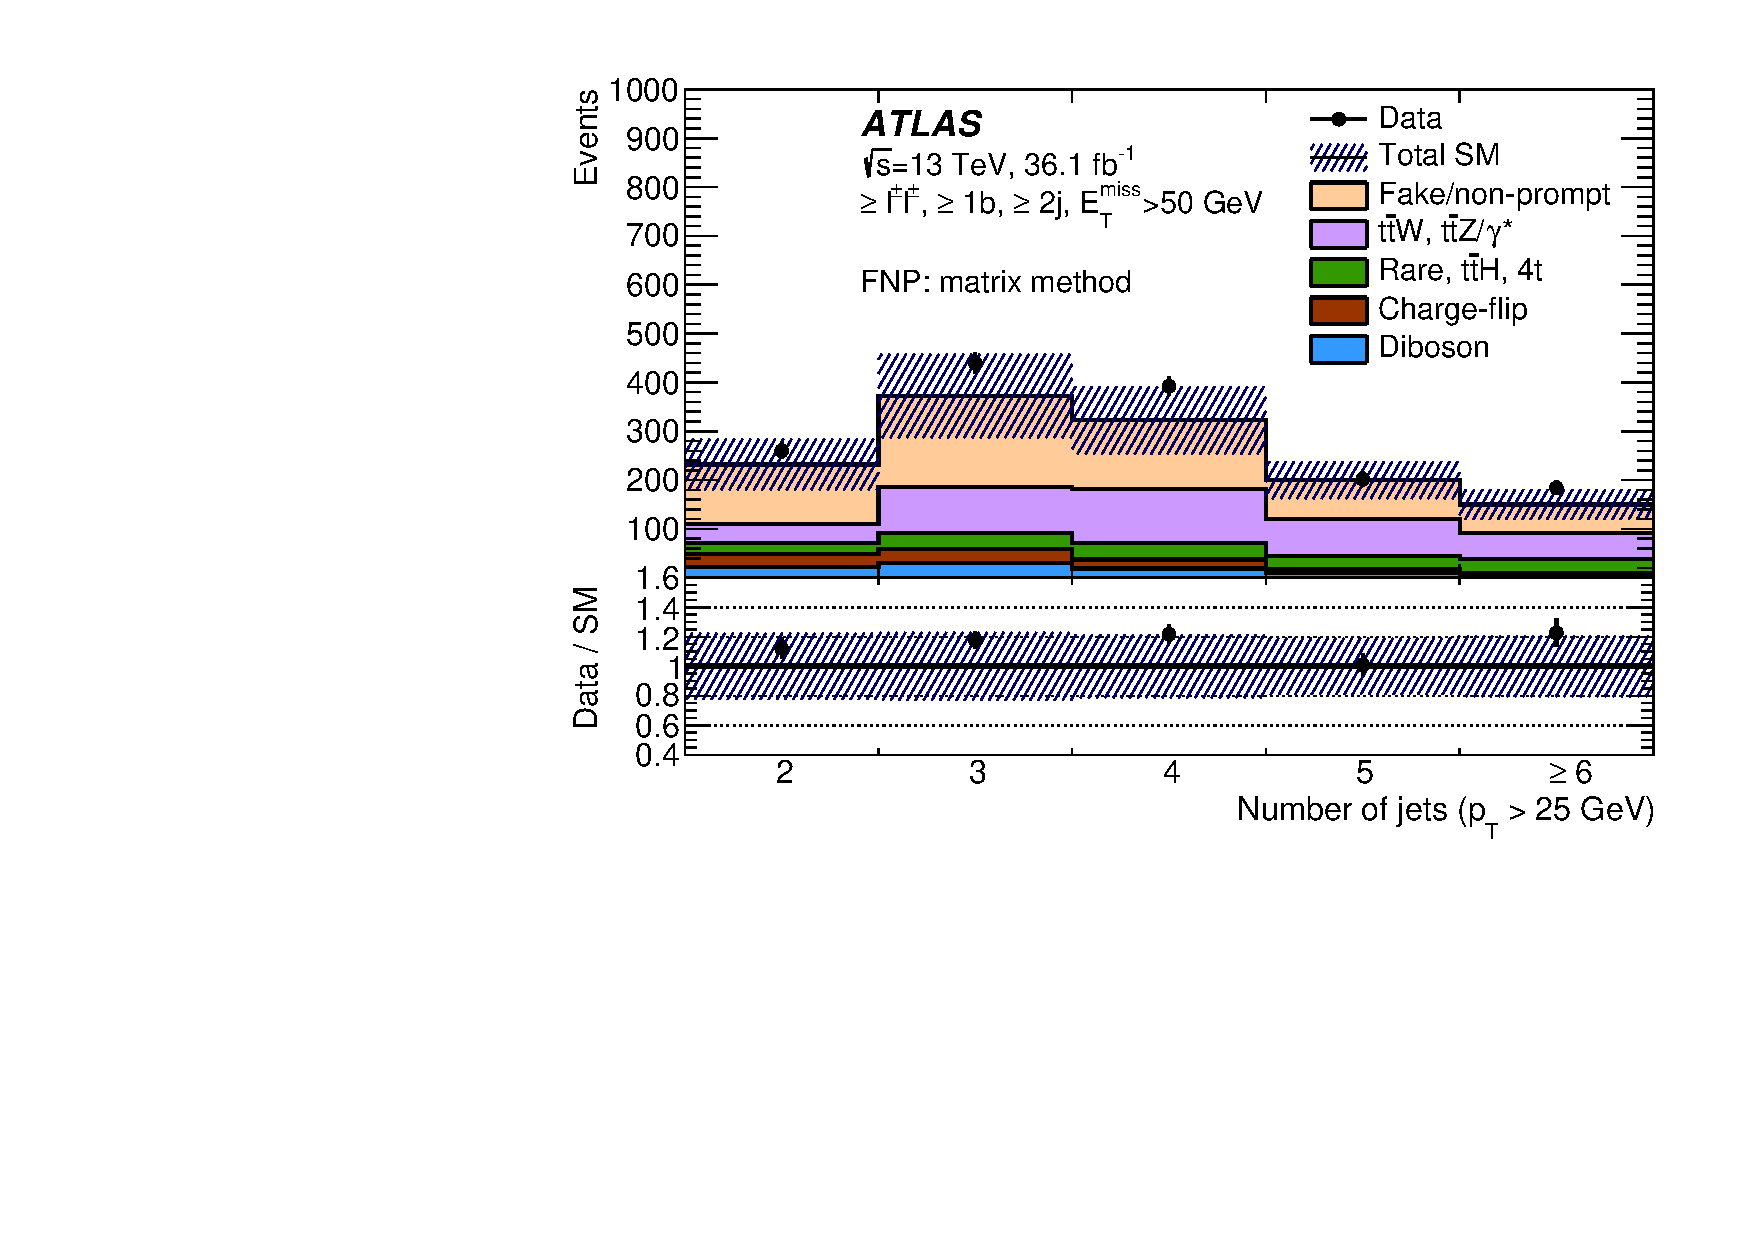
\includegraphics[width=\textwidth]{PAPER_DILEP_1B2JMET50_njets25_matrix}\caption{}\label{fig:VR1b2j_MxM}\end{subfigure}
\begin{subfigure}[t]{0.49\textwidth}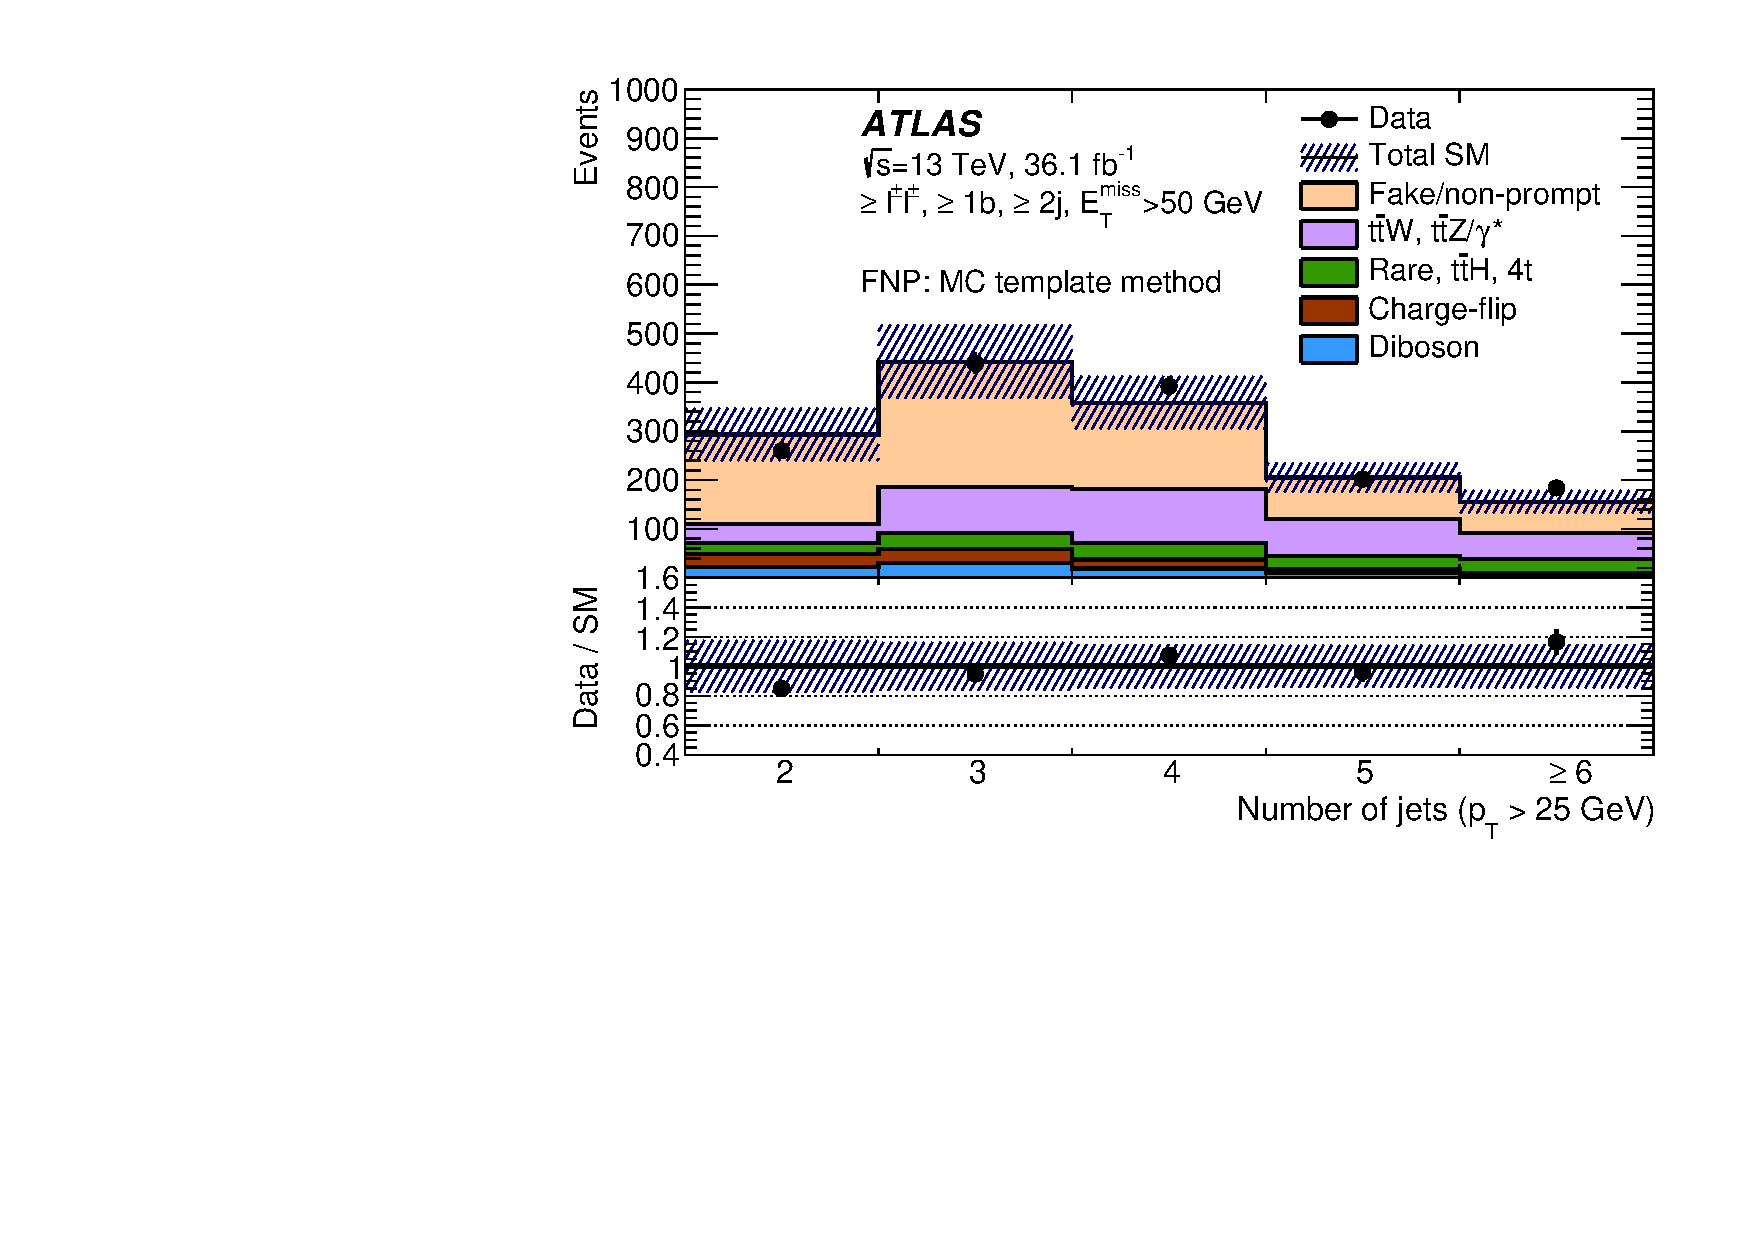
\includegraphics[width=\textwidth]{PAPER_DILEP_1B2JMET50_njets25_template}\caption{}\label{fig:VR1b2j_MCT}\end{subfigure}
\caption{
Distributions of the number of jets after requiring at least two jets ($\pT> 40 \GeV$) and $\met> 50 \GeV$, 
as well as at least two same-sign leptons. 
The fake or non-prompt leptons backgrounds are estimated alternatively with the matrix method (a) or the MC template method (b). 
The uncertainty band includes the statistical uncertainties for the background prediction as well as the
full systematic uncertainties for fake or non-prompt leptons backgrounds or charge-flip electrons. 
The rare category is defined in the text. In both figures, the last bin contains the overflow.
}
\label{fig:VR1b2j}
\end{figure}

\begin{figure}[htb!]
\centering
\begin{subfigure}[t]{0.66\textwidth}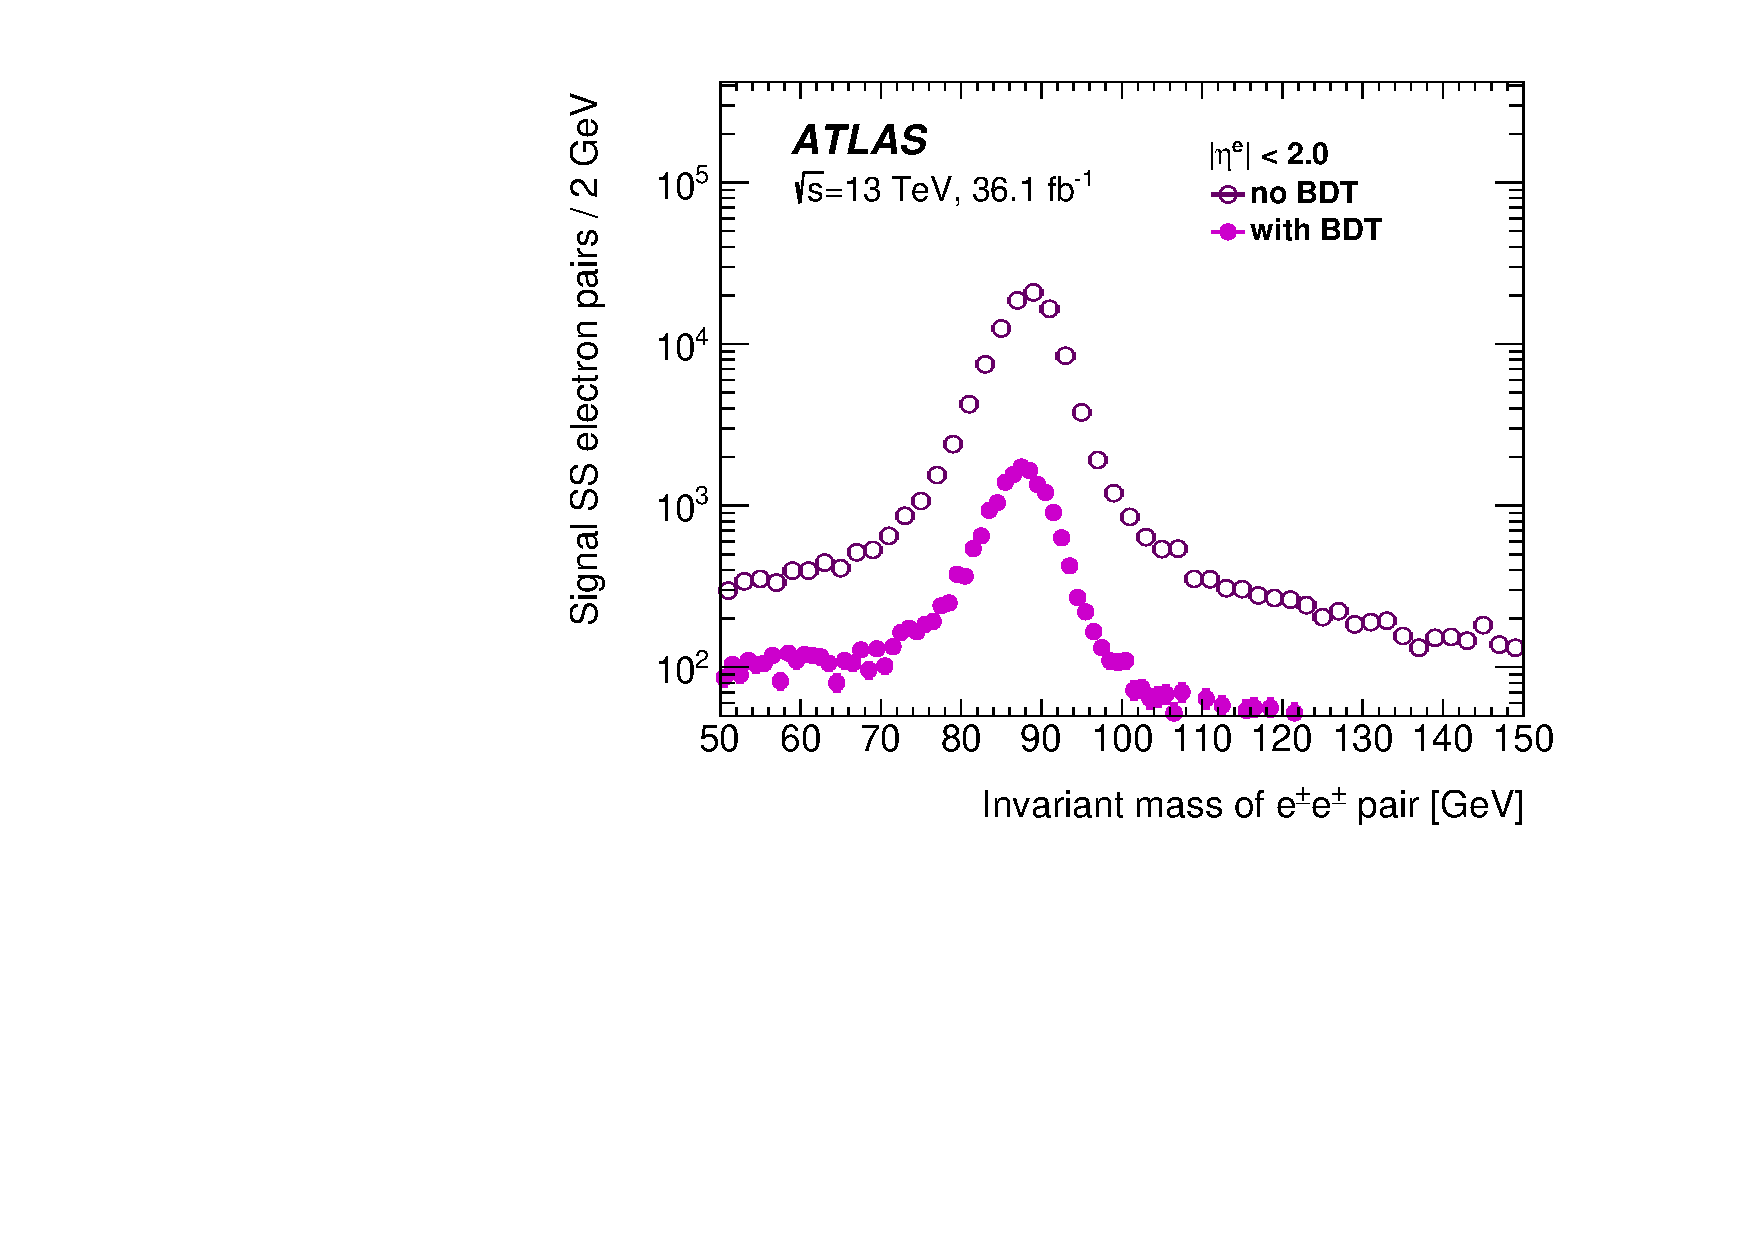
\includegraphics[width=\textwidth]{ETA_SS_BDTEL}\end{subfigure}
\caption{Invariant mass of the signal $e^{\pm} e^{\pm}$ pair distribution with (full markers) and without (open markers) charge-flip electron BDT selection applied.
}
\label{fig:ETA_SS_BDTEL}
\end{figure}
